% !TEX encoding = UTF-8 Unicode
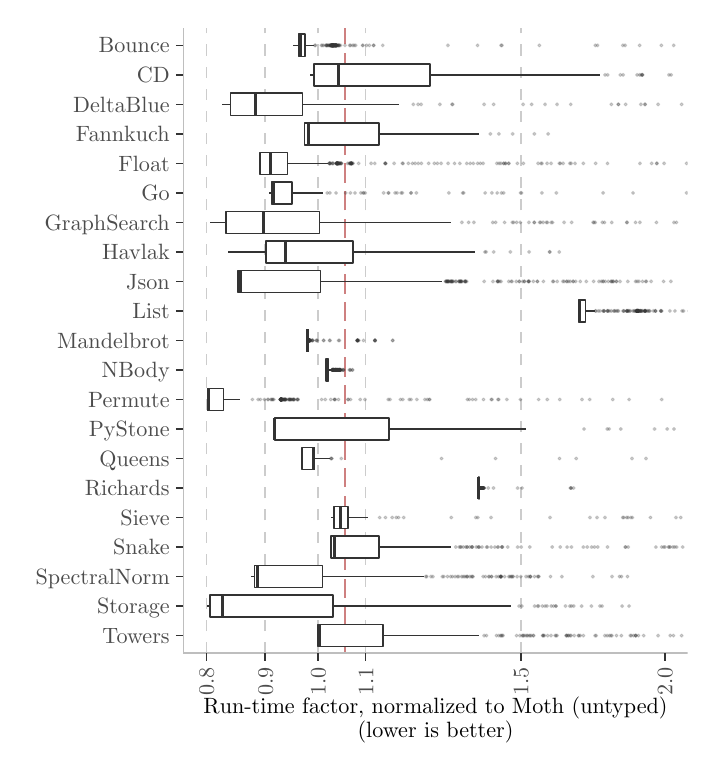
\begin{tikzpicture}[x=1pt,y=1pt]
\definecolor{fillColor}{RGB}{255,255,255}
\path[use as bounding box,fill=fillColor,fill opacity=0.00] (0,0) rectangle (238.49,260.17);
\begin{scope}
\path[clip] ( 56.27, 34.11) rectangle (238.49,260.17);
\definecolor{drawColor}{gray}{0.80}

\path[draw=drawColor,line width= 0.6pt,dash pattern=on 4pt off 4pt ,line join=round] ( 64.56, 34.11) -- ( 64.56,260.17);

\path[draw=drawColor,line width= 0.6pt,dash pattern=on 4pt off 4pt ,line join=round] ( 85.85, 34.11) -- ( 85.85,260.17);

\path[draw=drawColor,line width= 0.6pt,dash pattern=on 4pt off 4pt ,line join=round] (104.90, 34.11) -- (104.90,260.17);

\path[draw=drawColor,line width= 0.6pt,dash pattern=on 4pt off 4pt ,line join=round] (122.13, 34.11) -- (122.13,260.17);

\path[draw=drawColor,line width= 0.6pt,dash pattern=on 4pt off 4pt ,line join=round] (178.20, 34.11) -- (178.20,260.17);
\definecolor{drawColor}{RGB}{206,128,128}

\path[draw=drawColor,line width= 0.6pt,dash pattern=on 7pt off 3pt ,line join=round] (114.73, 34.11) -- (114.73,260.17);
\definecolor{drawColor}{RGB}{51,51,51}
\definecolor{fillColor}{RGB}{51,51,51}

\path[draw=drawColor,draw opacity=0.20,line width= 0.4pt,line join=round,line cap=round,fill=fillColor,fill opacity=0.20] (219.78, 40.51) circle (  0.57);

\path[draw=drawColor,draw opacity=0.20,line width= 0.4pt,line join=round,line cap=round,fill=fillColor,fill opacity=0.20] (214.53, 40.51) circle (  0.57);

\path[draw=drawColor,draw opacity=0.20,line width= 0.4pt,line join=round,line cap=round,fill=fillColor,fill opacity=0.20] (170.27, 40.51) circle (  0.57);

\path[draw=drawColor,draw opacity=0.20,line width= 0.4pt,line join=round,line cap=round,fill=fillColor,fill opacity=0.20] (187.89, 40.51) circle (  0.57);

\path[draw=drawColor,draw opacity=0.20,line width= 0.4pt,line join=round,line cap=round,fill=fillColor,fill opacity=0.20] (177.86, 40.51) circle (  0.57);

\path[draw=drawColor,draw opacity=0.20,line width= 0.4pt,line join=round,line cap=round,fill=fillColor,fill opacity=0.20] (236.29, 40.51) circle (  0.57);

\path[draw=drawColor,draw opacity=0.20,line width= 0.4pt,line join=round,line cap=round,fill=fillColor,fill opacity=0.20] (165.78, 40.51) circle (  0.57);

\path[draw=drawColor,draw opacity=0.20,line width= 0.4pt,line join=round,line cap=round,fill=fillColor,fill opacity=0.20] (171.75, 40.51) circle (  0.57);

\path[draw=drawColor,draw opacity=0.20,line width= 0.4pt,line join=round,line cap=round,fill=fillColor,fill opacity=0.20] (227.80, 40.51) circle (  0.57);

\path[draw=drawColor,draw opacity=0.20,line width= 0.4pt,line join=round,line cap=round,fill=fillColor,fill opacity=0.20] (190.95, 40.51) circle (  0.57);

\path[draw=drawColor,draw opacity=0.20,line width= 0.4pt,line join=round,line cap=round,fill=fillColor,fill opacity=0.20] (198.99, 40.51) circle (  0.57);

\path[draw=drawColor,draw opacity=0.20,line width= 0.4pt,line join=round,line cap=round,fill=fillColor,fill opacity=0.20] (189.11, 40.51) circle (  0.57);

\path[draw=drawColor,draw opacity=0.20,line width= 0.4pt,line join=round,line cap=round,fill=fillColor,fill opacity=0.20] (232.19, 40.51) circle (  0.57);

\path[draw=drawColor,draw opacity=0.20,line width= 0.4pt,line join=round,line cap=round,fill=fillColor,fill opacity=0.20] (233.34, 40.51) circle (  0.57);

\path[draw=drawColor,draw opacity=0.20,line width= 0.4pt,line join=round,line cap=round,fill=fillColor,fill opacity=0.20] (180.36, 40.51) circle (  0.57);

\path[draw=drawColor,draw opacity=0.20,line width= 0.4pt,line join=round,line cap=round,fill=fillColor,fill opacity=0.20] (180.56, 40.51) circle (  0.57);

\path[draw=drawColor,draw opacity=0.20,line width= 0.4pt,line join=round,line cap=round,fill=fillColor,fill opacity=0.20] (199.19, 40.51) circle (  0.57);

\path[draw=drawColor,draw opacity=0.20,line width= 0.4pt,line join=round,line cap=round,fill=fillColor,fill opacity=0.20] (210.18, 40.51) circle (  0.57);

\path[draw=drawColor,draw opacity=0.20,line width= 0.4pt,line join=round,line cap=round,fill=fillColor,fill opacity=0.20] (205.06, 40.51) circle (  0.57);

\path[draw=drawColor,draw opacity=0.20,line width= 0.4pt,line join=round,line cap=round,fill=fillColor,fill opacity=0.20] (199.67, 40.51) circle (  0.57);

\path[draw=drawColor,draw opacity=0.20,line width= 0.4pt,line join=round,line cap=round,fill=fillColor,fill opacity=0.20] (209.38, 40.51) circle (  0.57);

\path[draw=drawColor,draw opacity=0.20,line width= 0.4pt,line join=round,line cap=round,fill=fillColor,fill opacity=0.20] (196.06, 40.51) circle (  0.57);

\path[draw=drawColor,draw opacity=0.20,line width= 0.4pt,line join=round,line cap=round,fill=fillColor,fill opacity=0.20] (179.15, 40.51) circle (  0.57);

\path[draw=drawColor,draw opacity=0.20,line width= 0.4pt,line join=round,line cap=round,fill=fillColor,fill opacity=0.20] (181.19, 40.51) circle (  0.57);

\path[draw=drawColor,draw opacity=0.20,line width= 0.4pt,line join=round,line cap=round,fill=fillColor,fill opacity=0.20] (219.65, 40.51) circle (  0.57);

\path[draw=drawColor,draw opacity=0.20,line width= 0.4pt,line join=round,line cap=round,fill=fillColor,fill opacity=0.20] (196.34, 40.51) circle (  0.57);

\path[draw=drawColor,draw opacity=0.20,line width= 0.4pt,line join=round,line cap=round,fill=fillColor,fill opacity=0.20] (195.32, 40.51) circle (  0.57);

\path[draw=drawColor,draw opacity=0.20,line width= 0.4pt,line join=round,line cap=round,fill=fillColor,fill opacity=0.20] (181.58, 40.51) circle (  0.57);

\path[draw=drawColor,draw opacity=0.20,line width= 0.4pt,line join=round,line cap=round,fill=fillColor,fill opacity=0.20] (179.02, 40.51) circle (  0.57);

\path[draw=drawColor,draw opacity=0.20,line width= 0.4pt,line join=round,line cap=round,fill=fillColor,fill opacity=0.20] (186.74, 40.51) circle (  0.57);

\path[draw=drawColor,draw opacity=0.20,line width= 0.4pt,line join=round,line cap=round,fill=fillColor,fill opacity=0.20] (212.76, 40.51) circle (  0.57);

\path[draw=drawColor,draw opacity=0.20,line width= 0.4pt,line join=round,line cap=round,fill=fillColor,fill opacity=0.20] (186.30, 40.51) circle (  0.57);

\path[draw=drawColor,draw opacity=0.20,line width= 0.4pt,line join=round,line cap=round,fill=fillColor,fill opacity=0.20] (182.68, 40.51) circle (  0.57);

\path[draw=drawColor,draw opacity=0.20,line width= 0.4pt,line join=round,line cap=round,fill=fillColor,fill opacity=0.20] (219.71, 40.51) circle (  0.57);

\path[draw=drawColor,draw opacity=0.20,line width= 0.4pt,line join=round,line cap=round,fill=fillColor,fill opacity=0.20] (217.75, 40.51) circle (  0.57);

\path[draw=drawColor,draw opacity=0.20,line width= 0.4pt,line join=round,line cap=round,fill=fillColor,fill opacity=0.20] (176.66, 40.51) circle (  0.57);

\path[draw=drawColor,draw opacity=0.20,line width= 0.4pt,line join=round,line cap=round,fill=fillColor,fill opacity=0.20] (186.05, 40.51) circle (  0.57);

\path[draw=drawColor,draw opacity=0.20,line width= 0.4pt,line join=round,line cap=round,fill=fillColor,fill opacity=0.20] (186.30, 40.51) circle (  0.57);

\path[draw=drawColor,draw opacity=0.20,line width= 0.4pt,line join=round,line cap=round,fill=fillColor,fill opacity=0.20] (210.75, 40.51) circle (  0.57);

\path[draw=drawColor,draw opacity=0.20,line width= 0.4pt,line join=round,line cap=round,fill=fillColor,fill opacity=0.20] (218.11, 40.51) circle (  0.57);

\path[draw=drawColor,draw opacity=0.20,line width= 0.4pt,line join=round,line cap=round,fill=fillColor,fill opacity=0.20] (182.81, 40.51) circle (  0.57);

\path[draw=drawColor,draw opacity=0.20,line width= 0.4pt,line join=round,line cap=round,fill=fillColor,fill opacity=0.20] (195.50, 40.51) circle (  0.57);

\path[draw=drawColor,draw opacity=0.20,line width= 0.4pt,line join=round,line cap=round,fill=fillColor,fill opacity=0.20] (170.98, 40.51) circle (  0.57);

\path[draw=drawColor,draw opacity=0.20,line width= 0.4pt,line join=round,line cap=round,fill=fillColor,fill opacity=0.20] (190.62, 40.51) circle (  0.57);

\path[draw=drawColor,draw opacity=0.20,line width= 0.4pt,line join=round,line cap=round,fill=fillColor,fill opacity=0.20] (179.70, 40.51) circle (  0.57);

\path[draw=drawColor,draw opacity=0.20,line width= 0.4pt,line join=round,line cap=round,fill=fillColor,fill opacity=0.20] (222.59, 40.51) circle (  0.57);

\path[draw=drawColor,draw opacity=0.20,line width= 0.4pt,line join=round,line cap=round,fill=fillColor,fill opacity=0.20] (211.09, 40.51) circle (  0.57);

\path[draw=drawColor,draw opacity=0.20,line width= 0.4pt,line join=round,line cap=round,fill=fillColor,fill opacity=0.20] (220.70, 40.51) circle (  0.57);

\path[draw=drawColor,draw opacity=0.20,line width= 0.4pt,line join=round,line cap=round,fill=fillColor,fill opacity=0.20] (205.42, 40.51) circle (  0.57);

\path[draw=drawColor,draw opacity=0.20,line width= 0.4pt,line join=round,line cap=round,fill=fillColor,fill opacity=0.20] (194.67, 40.51) circle (  0.57);

\path[draw=drawColor,draw opacity=0.20,line width= 0.4pt,line join=round,line cap=round,fill=fillColor,fill opacity=0.20] (200.81, 40.51) circle (  0.57);

\path[draw=drawColor,draw opacity=0.20,line width= 0.4pt,line join=round,line cap=round,fill=fillColor,fill opacity=0.20] (171.09, 40.51) circle (  0.57);

\path[draw=drawColor,draw opacity=0.20,line width= 0.4pt,line join=round,line cap=round,fill=fillColor,fill opacity=0.20] (164.94, 40.51) circle (  0.57);

\path[draw=drawColor,draw opacity=0.20,line width= 0.4pt,line join=round,line cap=round,fill=fillColor,fill opacity=0.20] (181.92, 40.51) circle (  0.57);

\path[draw=drawColor,draw opacity=0.20,line width= 0.4pt,line join=round,line cap=round,fill=fillColor,fill opacity=0.20] (191.29, 40.51) circle (  0.57);

\path[draw=drawColor,draw opacity=0.20,line width= 0.4pt,line join=round,line cap=round,fill=fillColor,fill opacity=0.20] (194.61, 40.51) circle (  0.57);

\path[draw=drawColor,draw opacity=0.20,line width= 0.4pt,line join=round,line cap=round,fill=fillColor,fill opacity=0.20] (218.92, 40.51) circle (  0.57);

\path[draw=drawColor,draw opacity=0.20,line width= 0.4pt,line join=round,line cap=round,fill=fillColor,fill opacity=0.20] (171.49, 40.51) circle (  0.57);

\path[draw=drawColor,draw opacity=0.20,line width= 0.4pt,line join=round,line cap=round,fill=fillColor,fill opacity=0.20] (208.56, 40.51) circle (  0.57);

\path[draw=drawColor,draw opacity=0.20,line width= 0.4pt,line join=round,line cap=round,fill=fillColor,fill opacity=0.20] (169.40, 40.51) circle (  0.57);

\path[draw=drawColor,draw opacity=0.20,line width= 0.4pt,line join=round,line cap=round,fill=fillColor,fill opacity=0.20] (197.49, 40.51) circle (  0.57);

\path[draw=drawColor,draw opacity=0.20,line width= 0.4pt,line join=round,line cap=round,fill=fillColor,fill opacity=0.20] (194.87, 40.51) circle (  0.57);

\path[draw=drawColor,draw opacity=0.20,line width= 0.4pt,line join=round,line cap=round,fill=fillColor,fill opacity=0.20] (178.68, 40.51) circle (  0.57);
\definecolor{drawColor}{gray}{0.20}

\path[draw=drawColor,line width= 0.6pt,line join=round] (128.49, 40.51) -- (163.19, 40.51);

\path[draw=drawColor,line width= 0.6pt,line join=round] (104.92, 40.51) -- (104.44, 40.51);
\definecolor{fillColor}{RGB}{255,255,255}

\path[draw=drawColor,line width= 0.6pt,line join=round,line cap=round,fill=fillColor] (128.49, 36.51) --
	(104.92, 36.51) --
	(104.92, 44.51) --
	(128.49, 44.51) --
	(128.49, 36.51) --
	cycle;

\path[draw=drawColor,line width= 1.1pt,line join=round] (105.49, 36.51) -- (105.49, 44.51);
\definecolor{drawColor}{RGB}{51,51,51}
\definecolor{fillColor}{RGB}{51,51,51}

\path[draw=drawColor,draw opacity=0.20,line width= 0.4pt,line join=round,line cap=round,fill=fillColor,fill opacity=0.20] (187.65, 51.17) circle (  0.57);

\path[draw=drawColor,draw opacity=0.20,line width= 0.4pt,line join=round,line cap=round,fill=fillColor,fill opacity=0.20] (177.56, 51.17) circle (  0.57);

\path[draw=drawColor,draw opacity=0.20,line width= 0.4pt,line join=round,line cap=round,fill=fillColor,fill opacity=0.20] (200.17, 51.17) circle (  0.57);

\path[draw=drawColor,draw opacity=0.20,line width= 0.4pt,line join=round,line cap=round,fill=fillColor,fill opacity=0.20] (186.96, 51.17) circle (  0.57);

\path[draw=drawColor,draw opacity=0.20,line width= 0.4pt,line join=round,line cap=round,fill=fillColor,fill opacity=0.20] (217.31, 51.17) circle (  0.57);

\path[draw=drawColor,draw opacity=0.20,line width= 0.4pt,line join=round,line cap=round,fill=fillColor,fill opacity=0.20] (195.92, 51.17) circle (  0.57);

\path[draw=drawColor,draw opacity=0.20,line width= 0.4pt,line join=round,line cap=round,fill=fillColor,fill opacity=0.20] (184.28, 51.17) circle (  0.57);

\path[draw=drawColor,draw opacity=0.20,line width= 0.4pt,line join=round,line cap=round,fill=fillColor,fill opacity=0.20] (184.59, 51.17) circle (  0.57);

\path[draw=drawColor,draw opacity=0.20,line width= 0.4pt,line join=round,line cap=round,fill=fillColor,fill opacity=0.20] (190.87, 51.17) circle (  0.57);

\path[draw=drawColor,draw opacity=0.20,line width= 0.4pt,line join=round,line cap=round,fill=fillColor,fill opacity=0.20] (189.19, 51.17) circle (  0.57);

\path[draw=drawColor,draw opacity=0.20,line width= 0.4pt,line join=round,line cap=round,fill=fillColor,fill opacity=0.20] (207.57, 51.17) circle (  0.57);

\path[draw=drawColor,draw opacity=0.20,line width= 0.4pt,line join=round,line cap=round,fill=fillColor,fill opacity=0.20] (183.19, 51.17) circle (  0.57);

\path[draw=drawColor,draw opacity=0.20,line width= 0.4pt,line join=round,line cap=round,fill=fillColor,fill opacity=0.20] (196.52, 51.17) circle (  0.57);

\path[draw=drawColor,draw opacity=0.20,line width= 0.4pt,line join=round,line cap=round,fill=fillColor,fill opacity=0.20] (178.57, 51.17) circle (  0.57);

\path[draw=drawColor,draw opacity=0.20,line width= 0.4pt,line join=round,line cap=round,fill=fillColor,fill opacity=0.20] (206.79, 51.17) circle (  0.57);

\path[draw=drawColor,draw opacity=0.20,line width= 0.4pt,line join=round,line cap=round,fill=fillColor,fill opacity=0.20] (190.03, 51.17) circle (  0.57);

\path[draw=drawColor,draw opacity=0.20,line width= 0.4pt,line join=round,line cap=round,fill=fillColor,fill opacity=0.20] (214.81, 51.17) circle (  0.57);

\path[draw=drawColor,draw opacity=0.20,line width= 0.4pt,line join=round,line cap=round,fill=fillColor,fill opacity=0.20] (190.88, 51.17) circle (  0.57);

\path[draw=drawColor,draw opacity=0.20,line width= 0.4pt,line join=round,line cap=round,fill=fillColor,fill opacity=0.20] (197.33, 51.17) circle (  0.57);

\path[draw=drawColor,draw opacity=0.20,line width= 0.4pt,line join=round,line cap=round,fill=fillColor,fill opacity=0.20] (186.00, 51.17) circle (  0.57);

\path[draw=drawColor,draw opacity=0.20,line width= 0.4pt,line join=round,line cap=round,fill=fillColor,fill opacity=0.20] (194.33, 51.17) circle (  0.57);

\path[draw=drawColor,draw opacity=0.20,line width= 0.4pt,line join=round,line cap=round,fill=fillColor,fill opacity=0.20] (203.71, 51.17) circle (  0.57);
\definecolor{drawColor}{gray}{0.20}

\path[draw=drawColor,line width= 0.6pt,line join=round] (110.29, 51.17) -- (174.66, 51.17);

\path[draw=drawColor,line width= 0.6pt,line join=round] ( 65.77, 51.17) -- ( 64.97, 51.17);
\definecolor{fillColor}{RGB}{255,255,255}

\path[draw=drawColor,line width= 0.6pt,line join=round,line cap=round,fill=fillColor] (110.29, 47.17) --
	( 65.77, 47.17) --
	( 65.77, 55.17) --
	(110.29, 55.17) --
	(110.29, 47.17) --
	cycle;

\path[draw=drawColor,line width= 1.1pt,line join=round] ( 70.40, 47.17) -- ( 70.40, 55.17);
\definecolor{drawColor}{RGB}{51,51,51}
\definecolor{fillColor}{RGB}{51,51,51}

\path[draw=drawColor,draw opacity=0.20,line width= 0.4pt,line join=round,line cap=round,fill=fillColor,fill opacity=0.20] (166.56, 61.83) circle (  0.57);

\path[draw=drawColor,draw opacity=0.20,line width= 0.4pt,line join=round,line cap=round,fill=fillColor,fill opacity=0.20] (160.75, 61.83) circle (  0.57);

\path[draw=drawColor,draw opacity=0.20,line width= 0.4pt,line join=round,line cap=round,fill=fillColor,fill opacity=0.20] (181.61, 61.83) circle (  0.57);

\path[draw=drawColor,draw opacity=0.20,line width= 0.4pt,line join=round,line cap=round,fill=fillColor,fill opacity=0.20] (175.38, 61.83) circle (  0.57);

\path[draw=drawColor,draw opacity=0.20,line width= 0.4pt,line join=round,line cap=round,fill=fillColor,fill opacity=0.20] (180.08, 61.83) circle (  0.57);

\path[draw=drawColor,draw opacity=0.20,line width= 0.4pt,line join=round,line cap=round,fill=fillColor,fill opacity=0.20] (184.60, 61.83) circle (  0.57);

\path[draw=drawColor,draw opacity=0.20,line width= 0.4pt,line join=round,line cap=round,fill=fillColor,fill opacity=0.20] (165.42, 61.83) circle (  0.57);

\path[draw=drawColor,draw opacity=0.20,line width= 0.4pt,line join=round,line cap=round,fill=fillColor,fill opacity=0.20] (157.86, 61.83) circle (  0.57);

\path[draw=drawColor,draw opacity=0.20,line width= 0.4pt,line join=round,line cap=round,fill=fillColor,fill opacity=0.20] (172.35, 61.83) circle (  0.57);

\path[draw=drawColor,draw opacity=0.20,line width= 0.4pt,line join=round,line cap=round,fill=fillColor,fill opacity=0.20] (155.27, 61.83) circle (  0.57);

\path[draw=drawColor,draw opacity=0.20,line width= 0.4pt,line join=round,line cap=round,fill=fillColor,fill opacity=0.20] (170.86, 61.83) circle (  0.57);

\path[draw=drawColor,draw opacity=0.20,line width= 0.4pt,line join=round,line cap=round,fill=fillColor,fill opacity=0.20] (158.89, 61.83) circle (  0.57);

\path[draw=drawColor,draw opacity=0.20,line width= 0.4pt,line join=round,line cap=round,fill=fillColor,fill opacity=0.20] (181.74, 61.83) circle (  0.57);

\path[draw=drawColor,draw opacity=0.20,line width= 0.4pt,line join=round,line cap=round,fill=fillColor,fill opacity=0.20] (213.85, 61.83) circle (  0.57);

\path[draw=drawColor,draw opacity=0.20,line width= 0.4pt,line join=round,line cap=round,fill=fillColor,fill opacity=0.20] (144.20, 61.83) circle (  0.57);

\path[draw=drawColor,draw opacity=0.20,line width= 0.4pt,line join=round,line cap=round,fill=fillColor,fill opacity=0.20] (171.02, 61.83) circle (  0.57);

\path[draw=drawColor,draw opacity=0.20,line width= 0.4pt,line join=round,line cap=round,fill=fillColor,fill opacity=0.20] (158.41, 61.83) circle (  0.57);

\path[draw=drawColor,draw opacity=0.20,line width= 0.4pt,line join=round,line cap=round,fill=fillColor,fill opacity=0.20] (155.75, 61.83) circle (  0.57);

\path[draw=drawColor,draw opacity=0.20,line width= 0.4pt,line join=round,line cap=round,fill=fillColor,fill opacity=0.20] (159.80, 61.83) circle (  0.57);

\path[draw=drawColor,draw opacity=0.20,line width= 0.4pt,line join=round,line cap=round,fill=fillColor,fill opacity=0.20] (214.58, 61.83) circle (  0.57);

\path[draw=drawColor,draw opacity=0.20,line width= 0.4pt,line join=round,line cap=round,fill=fillColor,fill opacity=0.20] (146.43, 61.83) circle (  0.57);

\path[draw=drawColor,draw opacity=0.20,line width= 0.4pt,line join=round,line cap=round,fill=fillColor,fill opacity=0.20] (160.35, 61.83) circle (  0.57);

\path[draw=drawColor,draw opacity=0.20,line width= 0.4pt,line join=round,line cap=round,fill=fillColor,fill opacity=0.20] (145.73, 61.83) circle (  0.57);

\path[draw=drawColor,draw opacity=0.20,line width= 0.4pt,line join=round,line cap=round,fill=fillColor,fill opacity=0.20] (174.68, 61.83) circle (  0.57);

\path[draw=drawColor,draw opacity=0.20,line width= 0.4pt,line join=round,line cap=round,fill=fillColor,fill opacity=0.20] (216.75, 61.83) circle (  0.57);

\path[draw=drawColor,draw opacity=0.20,line width= 0.4pt,line join=round,line cap=round,fill=fillColor,fill opacity=0.20] (166.83, 61.83) circle (  0.57);

\path[draw=drawColor,draw opacity=0.20,line width= 0.4pt,line join=round,line cap=round,fill=fillColor,fill opacity=0.20] (184.67, 61.83) circle (  0.57);

\path[draw=drawColor,draw opacity=0.20,line width= 0.4pt,line join=round,line cap=round,fill=fillColor,fill opacity=0.20] (183.15, 61.83) circle (  0.57);

\path[draw=drawColor,draw opacity=0.20,line width= 0.4pt,line join=round,line cap=round,fill=fillColor,fill opacity=0.20] (160.86, 61.83) circle (  0.57);

\path[draw=drawColor,draw opacity=0.20,line width= 0.4pt,line join=round,line cap=round,fill=fillColor,fill opacity=0.20] (184.21, 61.83) circle (  0.57);

\path[draw=drawColor,draw opacity=0.20,line width= 0.4pt,line join=round,line cap=round,fill=fillColor,fill opacity=0.20] (167.65, 61.83) circle (  0.57);

\path[draw=drawColor,draw opacity=0.20,line width= 0.4pt,line join=round,line cap=round,fill=fillColor,fill opacity=0.20] (169.28, 61.83) circle (  0.57);

\path[draw=drawColor,draw opacity=0.20,line width= 0.4pt,line join=round,line cap=round,fill=fillColor,fill opacity=0.20] (188.93, 61.83) circle (  0.57);

\path[draw=drawColor,draw opacity=0.20,line width= 0.4pt,line join=round,line cap=round,fill=fillColor,fill opacity=0.20] (174.22, 61.83) circle (  0.57);

\path[draw=drawColor,draw opacity=0.20,line width= 0.4pt,line join=round,line cap=round,fill=fillColor,fill opacity=0.20] (170.09, 61.83) circle (  0.57);

\path[draw=drawColor,draw opacity=0.20,line width= 0.4pt,line join=round,line cap=round,fill=fillColor,fill opacity=0.20] (170.99, 61.83) circle (  0.57);

\path[draw=drawColor,draw opacity=0.20,line width= 0.4pt,line join=round,line cap=round,fill=fillColor,fill opacity=0.20] (164.60, 61.83) circle (  0.57);

\path[draw=drawColor,draw opacity=0.20,line width= 0.4pt,line join=round,line cap=round,fill=fillColor,fill opacity=0.20] (204.22, 61.83) circle (  0.57);

\path[draw=drawColor,draw opacity=0.20,line width= 0.4pt,line join=round,line cap=round,fill=fillColor,fill opacity=0.20] (157.33, 61.83) circle (  0.57);

\path[draw=drawColor,draw opacity=0.20,line width= 0.4pt,line join=round,line cap=round,fill=fillColor,fill opacity=0.20] (151.70, 61.83) circle (  0.57);

\path[draw=drawColor,draw opacity=0.20,line width= 0.4pt,line join=round,line cap=round,fill=fillColor,fill opacity=0.20] (149.86, 61.83) circle (  0.57);

\path[draw=drawColor,draw opacity=0.20,line width= 0.4pt,line join=round,line cap=round,fill=fillColor,fill opacity=0.20] (152.84, 61.83) circle (  0.57);

\path[draw=drawColor,draw opacity=0.20,line width= 0.4pt,line join=round,line cap=round,fill=fillColor,fill opacity=0.20] (170.80, 61.83) circle (  0.57);

\path[draw=drawColor,draw opacity=0.20,line width= 0.4pt,line join=round,line cap=round,fill=fillColor,fill opacity=0.20] (167.62, 61.83) circle (  0.57);

\path[draw=drawColor,draw opacity=0.20,line width= 0.4pt,line join=round,line cap=round,fill=fillColor,fill opacity=0.20] (153.50, 61.83) circle (  0.57);

\path[draw=drawColor,draw opacity=0.20,line width= 0.4pt,line join=round,line cap=round,fill=fillColor,fill opacity=0.20] (181.56, 61.83) circle (  0.57);

\path[draw=drawColor,draw opacity=0.20,line width= 0.4pt,line join=round,line cap=round,fill=fillColor,fill opacity=0.20] (193.03, 61.83) circle (  0.57);

\path[draw=drawColor,draw opacity=0.20,line width= 0.4pt,line join=round,line cap=round,fill=fillColor,fill opacity=0.20] (176.86, 61.83) circle (  0.57);

\path[draw=drawColor,draw opacity=0.20,line width= 0.4pt,line join=round,line cap=round,fill=fillColor,fill opacity=0.20] (156.82, 61.83) circle (  0.57);

\path[draw=drawColor,draw opacity=0.20,line width= 0.4pt,line join=round,line cap=round,fill=fillColor,fill opacity=0.20] (173.86, 61.83) circle (  0.57);

\path[draw=drawColor,draw opacity=0.20,line width= 0.4pt,line join=round,line cap=round,fill=fillColor,fill opacity=0.20] (170.99, 61.83) circle (  0.57);

\path[draw=drawColor,draw opacity=0.20,line width= 0.4pt,line join=round,line cap=round,fill=fillColor,fill opacity=0.20] (174.81, 61.83) circle (  0.57);

\path[draw=drawColor,draw opacity=0.20,line width= 0.4pt,line join=round,line cap=round,fill=fillColor,fill opacity=0.20] (211.16, 61.83) circle (  0.57);

\path[draw=drawColor,draw opacity=0.20,line width= 0.4pt,line join=round,line cap=round,fill=fillColor,fill opacity=0.20] (175.30, 61.83) circle (  0.57);

\path[draw=drawColor,draw opacity=0.20,line width= 0.4pt,line join=round,line cap=round,fill=fillColor,fill opacity=0.20] (143.86, 61.83) circle (  0.57);

\path[draw=drawColor,draw opacity=0.20,line width= 0.4pt,line join=round,line cap=round,fill=fillColor,fill opacity=0.20] (171.24, 61.83) circle (  0.57);

\path[draw=drawColor,draw opacity=0.20,line width= 0.4pt,line join=round,line cap=round,fill=fillColor,fill opacity=0.20] (154.44, 61.83) circle (  0.57);

\path[draw=drawColor,draw opacity=0.20,line width= 0.4pt,line join=round,line cap=round,fill=fillColor,fill opacity=0.20] (158.82, 61.83) circle (  0.57);

\path[draw=drawColor,draw opacity=0.20,line width= 0.4pt,line join=round,line cap=round,fill=fillColor,fill opacity=0.20] (180.89, 61.83) circle (  0.57);

\path[draw=drawColor,draw opacity=0.20,line width= 0.4pt,line join=round,line cap=round,fill=fillColor,fill opacity=0.20] (150.37, 61.83) circle (  0.57);

\path[draw=drawColor,draw opacity=0.20,line width= 0.4pt,line join=round,line cap=round,fill=fillColor,fill opacity=0.20] (178.20, 61.83) circle (  0.57);
\definecolor{drawColor}{gray}{0.20}

\path[draw=drawColor,line width= 0.6pt,line join=round] (106.57, 61.83) -- (143.22, 61.83);

\path[draw=drawColor,line width= 0.6pt,line join=round] ( 82.00, 61.83) -- ( 80.68, 61.83);
\definecolor{fillColor}{RGB}{255,255,255}

\path[draw=drawColor,line width= 0.6pt,line join=round,line cap=round,fill=fillColor] (106.57, 57.83) --
	( 82.00, 57.83) --
	( 82.00, 65.83) --
	(106.57, 65.83) --
	(106.57, 57.83) --
	cycle;

\path[draw=drawColor,line width= 1.1pt,line join=round] ( 83.11, 57.83) -- ( 83.11, 65.83);
\definecolor{drawColor}{RGB}{51,51,51}
\definecolor{fillColor}{RGB}{51,51,51}

\path[draw=drawColor,draw opacity=0.20,line width= 0.4pt,line join=round,line cap=round,fill=fillColor,fill opacity=0.20] (231.58, 72.50) circle (  0.57);

\path[draw=drawColor,draw opacity=0.20,line width= 0.4pt,line join=round,line cap=round,fill=fillColor,fill opacity=0.20] (206.00, 72.50) circle (  0.57);

\path[draw=drawColor,draw opacity=0.20,line width= 0.4pt,line join=round,line cap=round,fill=fillColor,fill opacity=0.20] (209.52, 72.50) circle (  0.57);

\path[draw=drawColor,draw opacity=0.20,line width= 0.4pt,line join=round,line cap=round,fill=fillColor,fill opacity=0.20] (162.88, 72.50) circle (  0.57);

\path[draw=drawColor,draw opacity=0.20,line width= 0.4pt,line join=round,line cap=round,fill=fillColor,fill opacity=0.20] (156.40, 72.50) circle (  0.57);

\path[draw=drawColor,draw opacity=0.20,line width= 0.4pt,line join=round,line cap=round,fill=fillColor,fill opacity=0.20] (231.81, 72.50) circle (  0.57);

\path[draw=drawColor,draw opacity=0.20,line width= 0.4pt,line join=round,line cap=round,fill=fillColor,fill opacity=0.20] (159.75, 72.50) circle (  0.57);

\path[draw=drawColor,draw opacity=0.20,line width= 0.4pt,line join=round,line cap=round,fill=fillColor,fill opacity=0.20] (162.87, 72.50) circle (  0.57);

\path[draw=drawColor,draw opacity=0.20,line width= 0.4pt,line join=round,line cap=round,fill=fillColor,fill opacity=0.20] (157.38, 72.50) circle (  0.57);

\path[draw=drawColor,draw opacity=0.20,line width= 0.4pt,line join=round,line cap=round,fill=fillColor,fill opacity=0.20] (158.85, 72.50) circle (  0.57);

\path[draw=drawColor,draw opacity=0.20,line width= 0.4pt,line join=round,line cap=round,fill=fillColor,fill opacity=0.20] (160.65, 72.50) circle (  0.57);

\path[draw=drawColor,draw opacity=0.20,line width= 0.4pt,line join=round,line cap=round,fill=fillColor,fill opacity=0.20] (156.60, 72.50) circle (  0.57);

\path[draw=drawColor,draw opacity=0.20,line width= 0.4pt,line join=round,line cap=round,fill=fillColor,fill opacity=0.20] (158.28, 72.50) circle (  0.57);

\path[draw=drawColor,draw opacity=0.20,line width= 0.4pt,line join=round,line cap=round,fill=fillColor,fill opacity=0.20] (162.08, 72.50) circle (  0.57);

\path[draw=drawColor,draw opacity=0.20,line width= 0.4pt,line join=round,line cap=round,fill=fillColor,fill opacity=0.20] (216.05, 72.50) circle (  0.57);

\path[draw=drawColor,draw opacity=0.20,line width= 0.4pt,line join=round,line cap=round,fill=fillColor,fill opacity=0.20] (229.82, 72.50) circle (  0.57);

\path[draw=drawColor,draw opacity=0.20,line width= 0.4pt,line join=round,line cap=round,fill=fillColor,fill opacity=0.20] (160.47, 72.50) circle (  0.57);

\path[draw=drawColor,draw opacity=0.20,line width= 0.4pt,line join=round,line cap=round,fill=fillColor,fill opacity=0.20] (168.81, 72.50) circle (  0.57);

\path[draw=drawColor,draw opacity=0.20,line width= 0.4pt,line join=round,line cap=round,fill=fillColor,fill opacity=0.20] (173.45, 72.50) circle (  0.57);

\path[draw=drawColor,draw opacity=0.20,line width= 0.4pt,line join=round,line cap=round,fill=fillColor,fill opacity=0.20] (215.98, 72.50) circle (  0.57);

\path[draw=drawColor,draw opacity=0.20,line width= 0.4pt,line join=round,line cap=round,fill=fillColor,fill opacity=0.20] (166.11, 72.50) circle (  0.57);

\path[draw=drawColor,draw opacity=0.20,line width= 0.4pt,line join=round,line cap=round,fill=fillColor,fill opacity=0.20] (204.84, 72.50) circle (  0.57);

\path[draw=drawColor,draw opacity=0.20,line width= 0.4pt,line join=round,line cap=round,fill=fillColor,fill opacity=0.20] (234.50, 72.50) circle (  0.57);

\path[draw=drawColor,draw opacity=0.20,line width= 0.4pt,line join=round,line cap=round,fill=fillColor,fill opacity=0.20] (178.33, 72.50) circle (  0.57);

\path[draw=drawColor,draw opacity=0.20,line width= 0.4pt,line join=round,line cap=round,fill=fillColor,fill opacity=0.20] (232.19, 72.50) circle (  0.57);

\path[draw=drawColor,draw opacity=0.20,line width= 0.4pt,line join=round,line cap=round,fill=fillColor,fill opacity=0.20] (171.30, 72.50) circle (  0.57);

\path[draw=drawColor,draw opacity=0.20,line width= 0.4pt,line join=round,line cap=round,fill=fillColor,fill opacity=0.20] (236.67, 72.50) circle (  0.57);

\path[draw=drawColor,draw opacity=0.20,line width= 0.4pt,line join=round,line cap=round,fill=fillColor,fill opacity=0.20] (181.44, 72.50) circle (  0.57);

\path[draw=drawColor,draw opacity=0.20,line width= 0.4pt,line join=round,line cap=round,fill=fillColor,fill opacity=0.20] (171.57, 72.50) circle (  0.57);

\path[draw=drawColor,draw opacity=0.20,line width= 0.4pt,line join=round,line cap=round,fill=fillColor,fill opacity=0.20] (177.04, 72.50) circle (  0.57);

\path[draw=drawColor,draw opacity=0.20,line width= 0.4pt,line join=round,line cap=round,fill=fillColor,fill opacity=0.20] (158.79, 72.50) circle (  0.57);

\path[draw=drawColor,draw opacity=0.20,line width= 0.4pt,line join=round,line cap=round,fill=fillColor,fill opacity=0.20] (192.44, 72.50) circle (  0.57);

\path[draw=drawColor,draw opacity=0.20,line width= 0.4pt,line join=round,line cap=round,fill=fillColor,fill opacity=0.20] (167.48, 72.50) circle (  0.57);

\path[draw=drawColor,draw opacity=0.20,line width= 0.4pt,line join=round,line cap=round,fill=fillColor,fill opacity=0.20] (227.00, 72.50) circle (  0.57);

\path[draw=drawColor,draw opacity=0.20,line width= 0.4pt,line join=round,line cap=round,fill=fillColor,fill opacity=0.20] (216.99, 72.50) circle (  0.57);

\path[draw=drawColor,draw opacity=0.20,line width= 0.4pt,line join=round,line cap=round,fill=fillColor,fill opacity=0.20] (163.23, 72.50) circle (  0.57);

\path[draw=drawColor,draw opacity=0.20,line width= 0.4pt,line join=round,line cap=round,fill=fillColor,fill opacity=0.20] (160.65, 72.50) circle (  0.57);

\path[draw=drawColor,draw opacity=0.20,line width= 0.4pt,line join=round,line cap=round,fill=fillColor,fill opacity=0.20] (155.96, 72.50) circle (  0.57);

\path[draw=drawColor,draw opacity=0.20,line width= 0.4pt,line join=round,line cap=round,fill=fillColor,fill opacity=0.20] (233.20, 72.50) circle (  0.57);

\path[draw=drawColor,draw opacity=0.20,line width= 0.4pt,line join=round,line cap=round,fill=fillColor,fill opacity=0.20] (194.93, 72.50) circle (  0.57);

\path[draw=drawColor,draw opacity=0.20,line width= 0.4pt,line join=round,line cap=round,fill=fillColor,fill opacity=0.20] (229.09, 72.50) circle (  0.57);

\path[draw=drawColor,draw opacity=0.20,line width= 0.4pt,line join=round,line cap=round,fill=fillColor,fill opacity=0.20] (169.80, 72.50) circle (  0.57);

\path[draw=drawColor,draw opacity=0.20,line width= 0.4pt,line join=round,line cap=round,fill=fillColor,fill opacity=0.20] (170.08, 72.50) circle (  0.57);

\path[draw=drawColor,draw opacity=0.20,line width= 0.4pt,line join=round,line cap=round,fill=fillColor,fill opacity=0.20] (171.41, 72.50) circle (  0.57);

\path[draw=drawColor,draw opacity=0.20,line width= 0.4pt,line join=round,line cap=round,fill=fillColor,fill opacity=0.20] (189.54, 72.50) circle (  0.57);

\path[draw=drawColor,draw opacity=0.20,line width= 0.4pt,line join=round,line cap=round,fill=fillColor,fill opacity=0.20] (203.78, 72.50) circle (  0.57);

\path[draw=drawColor,draw opacity=0.20,line width= 0.4pt,line join=round,line cap=round,fill=fillColor,fill opacity=0.20] (230.29, 72.50) circle (  0.57);

\path[draw=drawColor,draw opacity=0.20,line width= 0.4pt,line join=round,line cap=round,fill=fillColor,fill opacity=0.20] (196.48, 72.50) circle (  0.57);

\path[draw=drawColor,draw opacity=0.20,line width= 0.4pt,line join=round,line cap=round,fill=fillColor,fill opacity=0.20] (165.84, 72.50) circle (  0.57);

\path[draw=drawColor,draw opacity=0.20,line width= 0.4pt,line join=round,line cap=round,fill=fillColor,fill opacity=0.20] (233.80, 72.50) circle (  0.57);

\path[draw=drawColor,draw opacity=0.20,line width= 0.4pt,line join=round,line cap=round,fill=fillColor,fill opacity=0.20] (200.80, 72.50) circle (  0.57);

\path[draw=drawColor,draw opacity=0.20,line width= 0.4pt,line join=round,line cap=round,fill=fillColor,fill opacity=0.20] (202.20, 72.50) circle (  0.57);

\path[draw=drawColor,draw opacity=0.20,line width= 0.4pt,line join=round,line cap=round,fill=fillColor,fill opacity=0.20] (164.20, 72.50) circle (  0.57);

\path[draw=drawColor,draw opacity=0.20,line width= 0.4pt,line join=round,line cap=round,fill=fillColor,fill opacity=0.20] (154.68, 72.50) circle (  0.57);
\definecolor{drawColor}{gray}{0.20}

\path[draw=drawColor,line width= 0.6pt,line join=round] (127.01, 72.50) -- (152.92, 72.50);

\path[draw=drawColor,line width= 0.6pt,line join=round] (109.55, 72.50) -- (109.14, 72.50);
\definecolor{fillColor}{RGB}{255,255,255}

\path[draw=drawColor,line width= 0.6pt,line join=round,line cap=round,fill=fillColor] (127.01, 68.50) --
	(109.55, 68.50) --
	(109.55, 76.50) --
	(127.01, 76.50) --
	(127.01, 68.50) --
	cycle;

\path[draw=drawColor,line width= 1.1pt,line join=round] (110.72, 68.50) -- (110.72, 76.50);
\definecolor{drawColor}{RGB}{51,51,51}
\definecolor{fillColor}{RGB}{51,51,51}

\path[draw=drawColor,draw opacity=0.20,line width= 0.4pt,line join=round,line cap=round,fill=fillColor,fill opacity=0.20] (215.41, 83.16) circle (  0.57);

\path[draw=drawColor,draw opacity=0.20,line width= 0.4pt,line join=round,line cap=round,fill=fillColor,fill opacity=0.20] (129.28, 83.16) circle (  0.57);

\path[draw=drawColor,draw opacity=0.20,line width= 0.4pt,line join=round,line cap=round,fill=fillColor,fill opacity=0.20] (216.46, 83.16) circle (  0.57);

\path[draw=drawColor,draw opacity=0.20,line width= 0.4pt,line join=round,line cap=round,fill=fillColor,fill opacity=0.20] (208.59, 83.16) circle (  0.57);

\path[draw=drawColor,draw opacity=0.20,line width= 0.4pt,line join=round,line cap=round,fill=fillColor,fill opacity=0.20] (218.51, 83.16) circle (  0.57);

\path[draw=drawColor,draw opacity=0.20,line width= 0.4pt,line join=round,line cap=round,fill=fillColor,fill opacity=0.20] (162.66, 83.16) circle (  0.57);

\path[draw=drawColor,draw opacity=0.20,line width= 0.4pt,line join=round,line cap=round,fill=fillColor,fill opacity=0.20] (131.72, 83.16) circle (  0.57);

\path[draw=drawColor,draw opacity=0.20,line width= 0.4pt,line join=round,line cap=round,fill=fillColor,fill opacity=0.20] (234.24, 83.16) circle (  0.57);

\path[draw=drawColor,draw opacity=0.20,line width= 0.4pt,line join=round,line cap=round,fill=fillColor,fill opacity=0.20] (215.03, 83.16) circle (  0.57);

\path[draw=drawColor,draw opacity=0.20,line width= 0.4pt,line join=round,line cap=round,fill=fillColor,fill opacity=0.20] (216.97, 83.16) circle (  0.57);

\path[draw=drawColor,draw opacity=0.20,line width= 0.4pt,line join=round,line cap=round,fill=fillColor,fill opacity=0.20] (135.87, 83.16) circle (  0.57);

\path[draw=drawColor,draw opacity=0.20,line width= 0.4pt,line join=round,line cap=round,fill=fillColor,fill opacity=0.20] (188.76, 83.16) circle (  0.57);

\path[draw=drawColor,draw opacity=0.20,line width= 0.4pt,line join=round,line cap=round,fill=fillColor,fill opacity=0.20] (167.44, 83.16) circle (  0.57);

\path[draw=drawColor,draw opacity=0.20,line width= 0.4pt,line join=round,line cap=round,fill=fillColor,fill opacity=0.20] (225.04, 83.16) circle (  0.57);

\path[draw=drawColor,draw opacity=0.20,line width= 0.4pt,line join=round,line cap=round,fill=fillColor,fill opacity=0.20] (133.19, 83.16) circle (  0.57);

\path[draw=drawColor,draw opacity=0.20,line width= 0.4pt,line join=round,line cap=round,fill=fillColor,fill opacity=0.20] (127.19, 83.16) circle (  0.57);

\path[draw=drawColor,draw opacity=0.20,line width= 0.4pt,line join=round,line cap=round,fill=fillColor,fill opacity=0.20] (203.17, 83.16) circle (  0.57);

\path[draw=drawColor,draw opacity=0.20,line width= 0.4pt,line join=round,line cap=round,fill=fillColor,fill opacity=0.20] (153.07, 83.16) circle (  0.57);

\path[draw=drawColor,draw opacity=0.20,line width= 0.4pt,line join=round,line cap=round,fill=fillColor,fill opacity=0.20] (205.75, 83.16) circle (  0.57);

\path[draw=drawColor,draw opacity=0.20,line width= 0.4pt,line join=round,line cap=round,fill=fillColor,fill opacity=0.20] (161.93, 83.16) circle (  0.57);

\path[draw=drawColor,draw opacity=0.20,line width= 0.4pt,line join=round,line cap=round,fill=fillColor,fill opacity=0.20] (235.97, 83.16) circle (  0.57);

\path[draw=drawColor,draw opacity=0.20,line width= 0.4pt,line join=round,line cap=round,fill=fillColor,fill opacity=0.20] (134.01, 83.16) circle (  0.57);

\path[draw=drawColor,draw opacity=0.20,line width= 0.4pt,line join=round,line cap=round,fill=fillColor,fill opacity=0.20] (217.97, 83.16) circle (  0.57);
\definecolor{drawColor}{gray}{0.20}

\path[draw=drawColor,line width= 0.6pt,line join=round] (115.74, 83.16) -- (122.96, 83.16);

\path[draw=drawColor,line width= 0.6pt,line join=round] (110.64, 83.16) -- (109.75, 83.16);
\definecolor{fillColor}{RGB}{255,255,255}

\path[draw=drawColor,line width= 0.6pt,line join=round,line cap=round,fill=fillColor] (115.74, 79.16) --
	(110.64, 79.16) --
	(110.64, 87.16) --
	(115.74, 87.16) --
	(115.74, 79.16) --
	cycle;

\path[draw=drawColor,line width= 1.1pt,line join=round] (113.05, 79.16) -- (113.05, 87.16);
\definecolor{drawColor}{RGB}{51,51,51}
\definecolor{fillColor}{RGB}{51,51,51}

\path[draw=drawColor,draw opacity=0.20,line width= 0.4pt,line join=round,line cap=round,fill=fillColor,fill opacity=0.20] (164.01, 93.82) circle (  0.57);

\path[draw=drawColor,draw opacity=0.20,line width= 0.4pt,line join=round,line cap=round,fill=fillColor,fill opacity=0.20] (163.63, 93.82) circle (  0.57);

\path[draw=drawColor,draw opacity=0.20,line width= 0.4pt,line join=round,line cap=round,fill=fillColor,fill opacity=0.20] (164.14, 93.82) circle (  0.57);

\path[draw=drawColor,draw opacity=0.20,line width= 0.4pt,line join=round,line cap=round,fill=fillColor,fill opacity=0.20] (163.67, 93.82) circle (  0.57);

\path[draw=drawColor,draw opacity=0.20,line width= 0.4pt,line join=round,line cap=round,fill=fillColor,fill opacity=0.20] (197.26, 93.82) circle (  0.57);

\path[draw=drawColor,draw opacity=0.20,line width= 0.4pt,line join=round,line cap=round,fill=fillColor,fill opacity=0.20] (163.54, 93.82) circle (  0.57);

\path[draw=drawColor,draw opacity=0.20,line width= 0.4pt,line join=round,line cap=round,fill=fillColor,fill opacity=0.20] (163.37, 93.82) circle (  0.57);

\path[draw=drawColor,draw opacity=0.20,line width= 0.4pt,line join=round,line cap=round,fill=fillColor,fill opacity=0.20] (164.17, 93.82) circle (  0.57);

\path[draw=drawColor,draw opacity=0.20,line width= 0.4pt,line join=round,line cap=round,fill=fillColor,fill opacity=0.20] (163.71, 93.82) circle (  0.57);

\path[draw=drawColor,draw opacity=0.20,line width= 0.4pt,line join=round,line cap=round,fill=fillColor,fill opacity=0.20] (164.62, 93.82) circle (  0.57);

\path[draw=drawColor,draw opacity=0.20,line width= 0.4pt,line join=round,line cap=round,fill=fillColor,fill opacity=0.20] (164.28, 93.82) circle (  0.57);

\path[draw=drawColor,draw opacity=0.20,line width= 0.4pt,line join=round,line cap=round,fill=fillColor,fill opacity=0.20] (196.12, 93.82) circle (  0.57);

\path[draw=drawColor,draw opacity=0.20,line width= 0.4pt,line join=round,line cap=round,fill=fillColor,fill opacity=0.20] (196.28, 93.82) circle (  0.57);

\path[draw=drawColor,draw opacity=0.20,line width= 0.4pt,line join=round,line cap=round,fill=fillColor,fill opacity=0.20] (163.45, 93.82) circle (  0.57);

\path[draw=drawColor,draw opacity=0.20,line width= 0.4pt,line join=round,line cap=round,fill=fillColor,fill opacity=0.20] (163.46, 93.82) circle (  0.57);

\path[draw=drawColor,draw opacity=0.20,line width= 0.4pt,line join=round,line cap=round,fill=fillColor,fill opacity=0.20] (164.86, 93.82) circle (  0.57);

\path[draw=drawColor,draw opacity=0.20,line width= 0.4pt,line join=round,line cap=round,fill=fillColor,fill opacity=0.20] (164.03, 93.82) circle (  0.57);

\path[draw=drawColor,draw opacity=0.20,line width= 0.4pt,line join=round,line cap=round,fill=fillColor,fill opacity=0.20] (164.78, 93.82) circle (  0.57);

\path[draw=drawColor,draw opacity=0.20,line width= 0.4pt,line join=round,line cap=round,fill=fillColor,fill opacity=0.20] (163.60, 93.82) circle (  0.57);

\path[draw=drawColor,draw opacity=0.20,line width= 0.4pt,line join=round,line cap=round,fill=fillColor,fill opacity=0.20] (164.16, 93.82) circle (  0.57);

\path[draw=drawColor,draw opacity=0.20,line width= 0.4pt,line join=round,line cap=round,fill=fillColor,fill opacity=0.20] (196.38, 93.82) circle (  0.57);

\path[draw=drawColor,draw opacity=0.20,line width= 0.4pt,line join=round,line cap=round,fill=fillColor,fill opacity=0.20] (164.15, 93.82) circle (  0.57);

\path[draw=drawColor,draw opacity=0.20,line width= 0.4pt,line join=round,line cap=round,fill=fillColor,fill opacity=0.20] (164.91, 93.82) circle (  0.57);

\path[draw=drawColor,draw opacity=0.20,line width= 0.4pt,line join=round,line cap=round,fill=fillColor,fill opacity=0.20] (163.82, 93.82) circle (  0.57);

\path[draw=drawColor,draw opacity=0.20,line width= 0.4pt,line join=round,line cap=round,fill=fillColor,fill opacity=0.20] (163.65, 93.82) circle (  0.57);

\path[draw=drawColor,draw opacity=0.20,line width= 0.4pt,line join=round,line cap=round,fill=fillColor,fill opacity=0.20] (164.15, 93.82) circle (  0.57);

\path[draw=drawColor,draw opacity=0.20,line width= 0.4pt,line join=round,line cap=round,fill=fillColor,fill opacity=0.20] (163.79, 93.82) circle (  0.57);

\path[draw=drawColor,draw opacity=0.20,line width= 0.4pt,line join=round,line cap=round,fill=fillColor,fill opacity=0.20] (164.47, 93.82) circle (  0.57);

\path[draw=drawColor,draw opacity=0.20,line width= 0.4pt,line join=round,line cap=round,fill=fillColor,fill opacity=0.20] (178.66, 93.82) circle (  0.57);

\path[draw=drawColor,draw opacity=0.20,line width= 0.4pt,line join=round,line cap=round,fill=fillColor,fill opacity=0.20] (164.09, 93.82) circle (  0.57);

\path[draw=drawColor,draw opacity=0.20,line width= 0.4pt,line join=round,line cap=round,fill=fillColor,fill opacity=0.20] (163.65, 93.82) circle (  0.57);

\path[draw=drawColor,draw opacity=0.20,line width= 0.4pt,line join=round,line cap=round,fill=fillColor,fill opacity=0.20] (164.09, 93.82) circle (  0.57);

\path[draw=drawColor,draw opacity=0.20,line width= 0.4pt,line join=round,line cap=round,fill=fillColor,fill opacity=0.20] (163.84, 93.82) circle (  0.57);

\path[draw=drawColor,draw opacity=0.20,line width= 0.4pt,line join=round,line cap=round,fill=fillColor,fill opacity=0.20] (164.31, 93.82) circle (  0.57);

\path[draw=drawColor,draw opacity=0.20,line width= 0.4pt,line join=round,line cap=round,fill=fillColor,fill opacity=0.20] (163.51, 93.82) circle (  0.57);

\path[draw=drawColor,draw opacity=0.20,line width= 0.4pt,line join=round,line cap=round,fill=fillColor,fill opacity=0.20] (164.02, 93.82) circle (  0.57);

\path[draw=drawColor,draw opacity=0.20,line width= 0.4pt,line join=round,line cap=round,fill=fillColor,fill opacity=0.20] (168.33, 93.82) circle (  0.57);

\path[draw=drawColor,draw opacity=0.20,line width= 0.4pt,line join=round,line cap=round,fill=fillColor,fill opacity=0.20] (163.59, 93.82) circle (  0.57);

\path[draw=drawColor,draw opacity=0.20,line width= 0.4pt,line join=round,line cap=round,fill=fillColor,fill opacity=0.20] (164.15, 93.82) circle (  0.57);

\path[draw=drawColor,draw opacity=0.20,line width= 0.4pt,line join=round,line cap=round,fill=fillColor,fill opacity=0.20] (164.83, 93.82) circle (  0.57);

\path[draw=drawColor,draw opacity=0.20,line width= 0.4pt,line join=round,line cap=round,fill=fillColor,fill opacity=0.20] (163.37, 93.82) circle (  0.57);

\path[draw=drawColor,draw opacity=0.20,line width= 0.4pt,line join=round,line cap=round,fill=fillColor,fill opacity=0.20] (164.05, 93.82) circle (  0.57);

\path[draw=drawColor,draw opacity=0.20,line width= 0.4pt,line join=round,line cap=round,fill=fillColor,fill opacity=0.20] (163.55, 93.82) circle (  0.57);

\path[draw=drawColor,draw opacity=0.20,line width= 0.4pt,line join=round,line cap=round,fill=fillColor,fill opacity=0.20] (164.10, 93.82) circle (  0.57);

\path[draw=drawColor,draw opacity=0.20,line width= 0.4pt,line join=round,line cap=round,fill=fillColor,fill opacity=0.20] (163.73, 93.82) circle (  0.57);

\path[draw=drawColor,draw opacity=0.20,line width= 0.4pt,line join=round,line cap=round,fill=fillColor,fill opacity=0.20] (164.38, 93.82) circle (  0.57);

\path[draw=drawColor,draw opacity=0.20,line width= 0.4pt,line join=round,line cap=round,fill=fillColor,fill opacity=0.20] (164.01, 93.82) circle (  0.57);

\path[draw=drawColor,draw opacity=0.20,line width= 0.4pt,line join=round,line cap=round,fill=fillColor,fill opacity=0.20] (163.60, 93.82) circle (  0.57);

\path[draw=drawColor,draw opacity=0.20,line width= 0.4pt,line join=round,line cap=round,fill=fillColor,fill opacity=0.20] (164.18, 93.82) circle (  0.57);

\path[draw=drawColor,draw opacity=0.20,line width= 0.4pt,line join=round,line cap=round,fill=fillColor,fill opacity=0.20] (163.83, 93.82) circle (  0.57);

\path[draw=drawColor,draw opacity=0.20,line width= 0.4pt,line join=round,line cap=round,fill=fillColor,fill opacity=0.20] (164.39, 93.82) circle (  0.57);

\path[draw=drawColor,draw opacity=0.20,line width= 0.4pt,line join=round,line cap=round,fill=fillColor,fill opacity=0.20] (164.01, 93.82) circle (  0.57);

\path[draw=drawColor,draw opacity=0.20,line width= 0.4pt,line join=round,line cap=round,fill=fillColor,fill opacity=0.20] (163.73, 93.82) circle (  0.57);

\path[draw=drawColor,draw opacity=0.20,line width= 0.4pt,line join=round,line cap=round,fill=fillColor,fill opacity=0.20] (164.21, 93.82) circle (  0.57);

\path[draw=drawColor,draw opacity=0.20,line width= 0.4pt,line join=round,line cap=round,fill=fillColor,fill opacity=0.20] (163.80, 93.82) circle (  0.57);

\path[draw=drawColor,draw opacity=0.20,line width= 0.4pt,line join=round,line cap=round,fill=fillColor,fill opacity=0.20] (164.44, 93.82) circle (  0.57);

\path[draw=drawColor,draw opacity=0.20,line width= 0.4pt,line join=round,line cap=round,fill=fillColor,fill opacity=0.20] (164.06, 93.82) circle (  0.57);

\path[draw=drawColor,draw opacity=0.20,line width= 0.4pt,line join=round,line cap=round,fill=fillColor,fill opacity=0.20] (163.63, 93.82) circle (  0.57);

\path[draw=drawColor,draw opacity=0.20,line width= 0.4pt,line join=round,line cap=round,fill=fillColor,fill opacity=0.20] (164.31, 93.82) circle (  0.57);

\path[draw=drawColor,draw opacity=0.20,line width= 0.4pt,line join=round,line cap=round,fill=fillColor,fill opacity=0.20] (163.90, 93.82) circle (  0.57);

\path[draw=drawColor,draw opacity=0.20,line width= 0.4pt,line join=round,line cap=round,fill=fillColor,fill opacity=0.20] (163.43, 93.82) circle (  0.57);

\path[draw=drawColor,draw opacity=0.20,line width= 0.4pt,line join=round,line cap=round,fill=fillColor,fill opacity=0.20] (177.04, 93.82) circle (  0.57);

\path[draw=drawColor,draw opacity=0.20,line width= 0.4pt,line join=round,line cap=round,fill=fillColor,fill opacity=0.20] (166.43, 93.82) circle (  0.57);

\path[draw=drawColor,draw opacity=0.20,line width= 0.4pt,line join=round,line cap=round,fill=fillColor,fill opacity=0.20] (163.49, 93.82) circle (  0.57);

\path[draw=drawColor,draw opacity=0.20,line width= 0.4pt,line join=round,line cap=round,fill=fillColor,fill opacity=0.20] (164.41, 93.82) circle (  0.57);

\path[draw=drawColor,draw opacity=0.20,line width= 0.4pt,line join=round,line cap=round,fill=fillColor,fill opacity=0.20] (163.31, 93.82) circle (  0.57);

\path[draw=drawColor,draw opacity=0.20,line width= 0.4pt,line join=round,line cap=round,fill=fillColor,fill opacity=0.20] (163.37, 93.82) circle (  0.57);

\path[draw=drawColor,draw opacity=0.20,line width= 0.4pt,line join=round,line cap=round,fill=fillColor,fill opacity=0.20] (163.37, 93.82) circle (  0.57);

\path[draw=drawColor,draw opacity=0.20,line width= 0.4pt,line join=round,line cap=round,fill=fillColor,fill opacity=0.20] (163.35, 93.82) circle (  0.57);

\path[draw=drawColor,draw opacity=0.20,line width= 0.4pt,line join=round,line cap=round,fill=fillColor,fill opacity=0.20] (163.36, 93.82) circle (  0.57);

\path[draw=drawColor,draw opacity=0.20,line width= 0.4pt,line join=round,line cap=round,fill=fillColor,fill opacity=0.20] (163.85, 93.82) circle (  0.57);

\path[draw=drawColor,draw opacity=0.20,line width= 0.4pt,line join=round,line cap=round,fill=fillColor,fill opacity=0.20] (163.47, 93.82) circle (  0.57);

\path[draw=drawColor,draw opacity=0.20,line width= 0.4pt,line join=round,line cap=round,fill=fillColor,fill opacity=0.20] (163.39, 93.82) circle (  0.57);

\path[draw=drawColor,draw opacity=0.20,line width= 0.4pt,line join=round,line cap=round,fill=fillColor,fill opacity=0.20] (163.41, 93.82) circle (  0.57);

\path[draw=drawColor,draw opacity=0.20,line width= 0.4pt,line join=round,line cap=round,fill=fillColor,fill opacity=0.20] (164.18, 93.82) circle (  0.57);

\path[draw=drawColor,draw opacity=0.20,line width= 0.4pt,line join=round,line cap=round,fill=fillColor,fill opacity=0.20] (164.73, 93.82) circle (  0.57);

\path[draw=drawColor,draw opacity=0.20,line width= 0.4pt,line join=round,line cap=round,fill=fillColor,fill opacity=0.20] (163.79, 93.82) circle (  0.57);

\path[draw=drawColor,draw opacity=0.20,line width= 0.4pt,line join=round,line cap=round,fill=fillColor,fill opacity=0.20] (164.64, 93.82) circle (  0.57);

\path[draw=drawColor,draw opacity=0.20,line width= 0.4pt,line join=round,line cap=round,fill=fillColor,fill opacity=0.20] (163.41, 93.82) circle (  0.57);

\path[draw=drawColor,draw opacity=0.20,line width= 0.4pt,line join=round,line cap=round,fill=fillColor,fill opacity=0.20] (164.35, 93.82) circle (  0.57);

\path[draw=drawColor,draw opacity=0.20,line width= 0.4pt,line join=round,line cap=round,fill=fillColor,fill opacity=0.20] (163.69, 93.82) circle (  0.57);

\path[draw=drawColor,draw opacity=0.20,line width= 0.4pt,line join=round,line cap=round,fill=fillColor,fill opacity=0.20] (164.19, 93.82) circle (  0.57);

\path[draw=drawColor,draw opacity=0.20,line width= 0.4pt,line join=round,line cap=round,fill=fillColor,fill opacity=0.20] (163.80, 93.82) circle (  0.57);

\path[draw=drawColor,draw opacity=0.20,line width= 0.4pt,line join=round,line cap=round,fill=fillColor,fill opacity=0.20] (164.46, 93.82) circle (  0.57);

\path[draw=drawColor,draw opacity=0.20,line width= 0.4pt,line join=round,line cap=round,fill=fillColor,fill opacity=0.20] (163.38, 93.82) circle (  0.57);

\path[draw=drawColor,draw opacity=0.20,line width= 0.4pt,line join=round,line cap=round,fill=fillColor,fill opacity=0.20] (163.31, 93.82) circle (  0.57);

\path[draw=drawColor,draw opacity=0.20,line width= 0.4pt,line join=round,line cap=round,fill=fillColor,fill opacity=0.20] (163.47, 93.82) circle (  0.57);

\path[draw=drawColor,draw opacity=0.20,line width= 0.4pt,line join=round,line cap=round,fill=fillColor,fill opacity=0.20] (163.38, 93.82) circle (  0.57);

\path[draw=drawColor,draw opacity=0.20,line width= 0.4pt,line join=round,line cap=round,fill=fillColor,fill opacity=0.20] (163.40, 93.82) circle (  0.57);

\path[draw=drawColor,draw opacity=0.20,line width= 0.4pt,line join=round,line cap=round,fill=fillColor,fill opacity=0.20] (163.31, 93.82) circle (  0.57);

\path[draw=drawColor,draw opacity=0.20,line width= 0.4pt,line join=round,line cap=round,fill=fillColor,fill opacity=0.20] (164.14, 93.82) circle (  0.57);

\path[draw=drawColor,draw opacity=0.20,line width= 0.4pt,line join=round,line cap=round,fill=fillColor,fill opacity=0.20] (163.64, 93.82) circle (  0.57);

\path[draw=drawColor,draw opacity=0.20,line width= 0.4pt,line join=round,line cap=round,fill=fillColor,fill opacity=0.20] (163.57, 93.82) circle (  0.57);

\path[draw=drawColor,draw opacity=0.20,line width= 0.4pt,line join=round,line cap=round,fill=fillColor,fill opacity=0.20] (164.18, 93.82) circle (  0.57);

\path[draw=drawColor,draw opacity=0.20,line width= 0.4pt,line join=round,line cap=round,fill=fillColor,fill opacity=0.20] (163.73, 93.82) circle (  0.57);

\path[draw=drawColor,draw opacity=0.20,line width= 0.4pt,line join=round,line cap=round,fill=fillColor,fill opacity=0.20] (164.47, 93.82) circle (  0.57);
\definecolor{drawColor}{gray}{0.20}

\path[draw=drawColor,line width= 0.6pt,line join=round] (163.14, 93.82) -- (163.28, 93.82);

\path[draw=drawColor,line width= 0.6pt,line join=round] (163.04, 93.82) -- (162.95, 93.82);
\definecolor{fillColor}{RGB}{255,255,255}

\path[draw=drawColor,line width= 0.6pt,line join=round,line cap=round,fill=fillColor] (163.14, 89.82) --
	(163.04, 89.82) --
	(163.04, 97.82) --
	(163.14, 97.82) --
	(163.14, 89.82) --
	cycle;

\path[draw=drawColor,line width= 1.1pt,line join=round] (163.07, 89.82) -- (163.07, 97.82);
\definecolor{drawColor}{RGB}{51,51,51}
\definecolor{fillColor}{RGB}{51,51,51}

\path[draw=drawColor,draw opacity=0.20,line width= 0.4pt,line join=round,line cap=round,fill=fillColor,fill opacity=0.20] (198.21,104.49) circle (  0.57);

\path[draw=drawColor,draw opacity=0.20,line width= 0.4pt,line join=round,line cap=round,fill=fillColor,fill opacity=0.20] (109.63,104.49) circle (  0.57);

\path[draw=drawColor,draw opacity=0.20,line width= 0.4pt,line join=round,line cap=round,fill=fillColor,fill opacity=0.20] (109.73,104.49) circle (  0.57);

\path[draw=drawColor,draw opacity=0.20,line width= 0.4pt,line join=round,line cap=round,fill=fillColor,fill opacity=0.20] (192.18,104.49) circle (  0.57);

\path[draw=drawColor,draw opacity=0.20,line width= 0.4pt,line join=round,line cap=round,fill=fillColor,fill opacity=0.20] (223.43,104.49) circle (  0.57);

\path[draw=drawColor,draw opacity=0.20,line width= 0.4pt,line join=round,line cap=round,fill=fillColor,fill opacity=0.20] (113.34,104.49) circle (  0.57);

\path[draw=drawColor,draw opacity=0.20,line width= 0.4pt,line join=round,line cap=round,fill=fillColor,fill opacity=0.20] (169.07,104.49) circle (  0.57);

\path[draw=drawColor,draw opacity=0.20,line width= 0.4pt,line join=round,line cap=round,fill=fillColor,fill opacity=0.20] (218.37,104.49) circle (  0.57);

\path[draw=drawColor,draw opacity=0.20,line width= 0.4pt,line join=round,line cap=round,fill=fillColor,fill opacity=0.20] (109.89,104.49) circle (  0.57);

\path[draw=drawColor,draw opacity=0.20,line width= 0.4pt,line join=round,line cap=round,fill=fillColor,fill opacity=0.20] (149.55,104.49) circle (  0.57);
\definecolor{drawColor}{gray}{0.20}

\path[draw=drawColor,line width= 0.6pt,line join=round] (103.36,104.49) -- (109.23,104.49);

\path[draw=drawColor,line width= 0.6pt,line join=round] ( 99.21,104.49) -- ( 99.02,104.49);
\definecolor{fillColor}{RGB}{255,255,255}

\path[draw=drawColor,line width= 0.6pt,line join=round,line cap=round,fill=fillColor] (103.36,100.49) --
	( 99.21,100.49) --
	( 99.21,108.49) --
	(103.36,108.49) --
	(103.36,100.49) --
	cycle;

\path[draw=drawColor,line width= 1.1pt,line join=round] (103.21,100.49) -- (103.21,108.49);
\definecolor{drawColor}{RGB}{51,51,51}
\definecolor{fillColor}{RGB}{51,51,51}

\path[draw=drawColor,draw opacity=0.20,line width= 0.4pt,line join=round,line cap=round,fill=fillColor,fill opacity=0.20] (231.08,115.15) circle (  0.57);

\path[draw=drawColor,draw opacity=0.20,line width= 0.4pt,line join=round,line cap=round,fill=fillColor,fill opacity=0.20] (226.53,115.15) circle (  0.57);

\path[draw=drawColor,draw opacity=0.20,line width= 0.4pt,line join=round,line cap=round,fill=fillColor,fill opacity=0.20] (210.11,115.15) circle (  0.57);

\path[draw=drawColor,draw opacity=0.20,line width= 0.4pt,line join=round,line cap=round,fill=fillColor,fill opacity=0.20] (214.33,115.15) circle (  0.57);

\path[draw=drawColor,draw opacity=0.20,line width= 0.4pt,line join=round,line cap=round,fill=fillColor,fill opacity=0.20] (201.06,115.15) circle (  0.57);

\path[draw=drawColor,draw opacity=0.20,line width= 0.4pt,line join=round,line cap=round,fill=fillColor,fill opacity=0.20] (233.54,115.15) circle (  0.57);

\path[draw=drawColor,draw opacity=0.20,line width= 0.4pt,line join=round,line cap=round,fill=fillColor,fill opacity=0.20] (209.44,115.15) circle (  0.57);
\definecolor{drawColor}{gray}{0.20}

\path[draw=drawColor,line width= 0.6pt,line join=round] (130.62,115.15) -- (180.24,115.15);

\path[draw=drawColor,line width= 0.6pt,line join=round] ( 89.17,115.15) -- ( 88.56,115.15);
\definecolor{fillColor}{RGB}{255,255,255}

\path[draw=drawColor,line width= 0.6pt,line join=round,line cap=round,fill=fillColor] (130.62,111.15) --
	( 89.17,111.15) --
	( 89.17,119.15) --
	(130.62,119.15) --
	(130.62,111.15) --
	cycle;

\path[draw=drawColor,line width= 1.1pt,line join=round] ( 89.34,111.15) -- ( 89.34,119.15);
\definecolor{drawColor}{RGB}{51,51,51}
\definecolor{fillColor}{RGB}{51,51,51}

\path[draw=drawColor,draw opacity=0.20,line width= 0.4pt,line join=round,line cap=round,fill=fillColor,fill opacity=0.20] (211.41,125.81) circle (  0.57);

\path[draw=drawColor,draw opacity=0.20,line width= 0.4pt,line join=round,line cap=round,fill=fillColor,fill opacity=0.20] ( 92.77,125.81) circle (  0.57);

\path[draw=drawColor,draw opacity=0.20,line width= 0.4pt,line join=round,line cap=round,fill=fillColor,fill opacity=0.20] ( 86.88,125.81) circle (  0.57);

\path[draw=drawColor,draw opacity=0.20,line width= 0.4pt,line join=round,line cap=round,fill=fillColor,fill opacity=0.20] (169.95,125.81) circle (  0.57);

\path[draw=drawColor,draw opacity=0.20,line width= 0.4pt,line join=round,line cap=round,fill=fillColor,fill opacity=0.20] (167.54,125.81) circle (  0.57);

\path[draw=drawColor,draw opacity=0.20,line width= 0.4pt,line join=round,line cap=round,fill=fillColor,fill opacity=0.20] ( 88.51,125.81) circle (  0.57);

\path[draw=drawColor,draw opacity=0.20,line width= 0.4pt,line join=round,line cap=round,fill=fillColor,fill opacity=0.20] ( 88.94,125.81) circle (  0.57);

\path[draw=drawColor,draw opacity=0.20,line width= 0.4pt,line join=round,line cap=round,fill=fillColor,fill opacity=0.20] ( 95.35,125.81) circle (  0.57);

\path[draw=drawColor,draw opacity=0.20,line width= 0.4pt,line join=round,line cap=round,fill=fillColor,fill opacity=0.20] (229.09,125.81) circle (  0.57);

\path[draw=drawColor,draw opacity=0.20,line width= 0.4pt,line join=round,line cap=round,fill=fillColor,fill opacity=0.20] ( 93.06,125.81) circle (  0.57);

\path[draw=drawColor,draw opacity=0.20,line width= 0.4pt,line join=round,line cap=round,fill=fillColor,fill opacity=0.20] ( 92.54,125.81) circle (  0.57);

\path[draw=drawColor,draw opacity=0.20,line width= 0.4pt,line join=round,line cap=round,fill=fillColor,fill opacity=0.20] ( 91.70,125.81) circle (  0.57);

\path[draw=drawColor,draw opacity=0.20,line width= 0.4pt,line join=round,line cap=round,fill=fillColor,fill opacity=0.20] ( 91.57,125.81) circle (  0.57);

\path[draw=drawColor,draw opacity=0.20,line width= 0.4pt,line join=round,line cap=round,fill=fillColor,fill opacity=0.20] ( 91.51,125.81) circle (  0.57);

\path[draw=drawColor,draw opacity=0.20,line width= 0.4pt,line join=round,line cap=round,fill=fillColor,fill opacity=0.20] ( 91.57,125.81) circle (  0.57);

\path[draw=drawColor,draw opacity=0.20,line width= 0.4pt,line join=round,line cap=round,fill=fillColor,fill opacity=0.20] ( 91.60,125.81) circle (  0.57);

\path[draw=drawColor,draw opacity=0.20,line width= 0.4pt,line join=round,line cap=round,fill=fillColor,fill opacity=0.20] ( 91.64,125.81) circle (  0.57);

\path[draw=drawColor,draw opacity=0.20,line width= 0.4pt,line join=round,line cap=round,fill=fillColor,fill opacity=0.20] ( 94.49,125.81) circle (  0.57);

\path[draw=drawColor,draw opacity=0.20,line width= 0.4pt,line join=round,line cap=round,fill=fillColor,fill opacity=0.20] ( 91.44,125.81) circle (  0.57);

\path[draw=drawColor,draw opacity=0.20,line width= 0.4pt,line join=round,line cap=round,fill=fillColor,fill opacity=0.20] (144.38,125.81) circle (  0.57);

\path[draw=drawColor,draw opacity=0.20,line width= 0.4pt,line join=round,line cap=round,fill=fillColor,fill opacity=0.20] (160.77,125.81) circle (  0.57);

\path[draw=drawColor,draw opacity=0.20,line width= 0.4pt,line join=round,line cap=round,fill=fillColor,fill opacity=0.20] (145.25,125.81) circle (  0.57);

\path[draw=drawColor,draw opacity=0.20,line width= 0.4pt,line join=round,line cap=round,fill=fillColor,fill opacity=0.20] (184.63,125.81) circle (  0.57);

\path[draw=drawColor,draw opacity=0.20,line width= 0.4pt,line join=round,line cap=round,fill=fillColor,fill opacity=0.20] (134.69,125.81) circle (  0.57);

\path[draw=drawColor,draw opacity=0.20,line width= 0.4pt,line join=round,line cap=round,fill=fillColor,fill opacity=0.20] ( 92.36,125.81) circle (  0.57);

\path[draw=drawColor,draw opacity=0.20,line width= 0.4pt,line join=round,line cap=round,fill=fillColor,fill opacity=0.20] ( 91.50,125.81) circle (  0.57);

\path[draw=drawColor,draw opacity=0.20,line width= 0.4pt,line join=round,line cap=round,fill=fillColor,fill opacity=0.20] ( 93.67,125.81) circle (  0.57);

\path[draw=drawColor,draw opacity=0.20,line width= 0.4pt,line join=round,line cap=round,fill=fillColor,fill opacity=0.20] ( 91.41,125.81) circle (  0.57);

\path[draw=drawColor,draw opacity=0.20,line width= 0.4pt,line join=round,line cap=round,fill=fillColor,fill opacity=0.20] ( 96.16,125.81) circle (  0.57);

\path[draw=drawColor,draw opacity=0.20,line width= 0.4pt,line join=round,line cap=round,fill=fillColor,fill opacity=0.20] ( 91.41,125.81) circle (  0.57);

\path[draw=drawColor,draw opacity=0.20,line width= 0.4pt,line join=round,line cap=round,fill=fillColor,fill opacity=0.20] ( 91.49,125.81) circle (  0.57);

\path[draw=drawColor,draw opacity=0.20,line width= 0.4pt,line join=round,line cap=round,fill=fillColor,fill opacity=0.20] ( 96.06,125.81) circle (  0.57);

\path[draw=drawColor,draw opacity=0.20,line width= 0.4pt,line join=round,line cap=round,fill=fillColor,fill opacity=0.20] ( 91.33,125.81) circle (  0.57);

\path[draw=drawColor,draw opacity=0.20,line width= 0.4pt,line join=round,line cap=round,fill=fillColor,fill opacity=0.20] ( 91.32,125.81) circle (  0.57);

\path[draw=drawColor,draw opacity=0.20,line width= 0.4pt,line join=round,line cap=round,fill=fillColor,fill opacity=0.20] ( 94.56,125.81) circle (  0.57);

\path[draw=drawColor,draw opacity=0.20,line width= 0.4pt,line join=round,line cap=round,fill=fillColor,fill opacity=0.20] (115.82,125.81) circle (  0.57);

\path[draw=drawColor,draw opacity=0.20,line width= 0.4pt,line join=round,line cap=round,fill=fillColor,fill opacity=0.20] (173.15,125.81) circle (  0.57);

\path[draw=drawColor,draw opacity=0.20,line width= 0.4pt,line join=round,line cap=round,fill=fillColor,fill opacity=0.20] ( 93.23,125.81) circle (  0.57);

\path[draw=drawColor,draw opacity=0.20,line width= 0.4pt,line join=round,line cap=round,fill=fillColor,fill opacity=0.20] ( 86.80,125.81) circle (  0.57);

\path[draw=drawColor,draw opacity=0.20,line width= 0.4pt,line join=round,line cap=round,fill=fillColor,fill opacity=0.20] (200.30,125.81) circle (  0.57);

\path[draw=drawColor,draw opacity=0.20,line width= 0.4pt,line join=round,line cap=round,fill=fillColor,fill opacity=0.20] ( 97.44,125.81) circle (  0.57);

\path[draw=drawColor,draw opacity=0.20,line width= 0.4pt,line join=round,line cap=round,fill=fillColor,fill opacity=0.20] ( 97.35,125.81) circle (  0.57);

\path[draw=drawColor,draw opacity=0.20,line width= 0.4pt,line join=round,line cap=round,fill=fillColor,fill opacity=0.20] ( 97.65,125.81) circle (  0.57);

\path[draw=drawColor,draw opacity=0.20,line width= 0.4pt,line join=round,line cap=round,fill=fillColor,fill opacity=0.20] (130.95,125.81) circle (  0.57);

\path[draw=drawColor,draw opacity=0.20,line width= 0.4pt,line join=round,line cap=round,fill=fillColor,fill opacity=0.20] ( 83.28,125.81) circle (  0.57);

\path[draw=drawColor,draw opacity=0.20,line width= 0.4pt,line join=round,line cap=round,fill=fillColor,fill opacity=0.20] (161.88,125.81) circle (  0.57);

\path[draw=drawColor,draw opacity=0.20,line width= 0.4pt,line join=round,line cap=round,fill=fillColor,fill opacity=0.20] ( 94.86,125.81) circle (  0.57);

\path[draw=drawColor,draw opacity=0.20,line width= 0.4pt,line join=round,line cap=round,fill=fillColor,fill opacity=0.20] ( 93.07,125.81) circle (  0.57);

\path[draw=drawColor,draw opacity=0.20,line width= 0.4pt,line join=round,line cap=round,fill=fillColor,fill opacity=0.20] ( 93.02,125.81) circle (  0.57);

\path[draw=drawColor,draw opacity=0.20,line width= 0.4pt,line join=round,line cap=round,fill=fillColor,fill opacity=0.20] ( 91.59,125.81) circle (  0.57);

\path[draw=drawColor,draw opacity=0.20,line width= 0.4pt,line join=round,line cap=round,fill=fillColor,fill opacity=0.20] ( 91.80,125.81) circle (  0.57);

\path[draw=drawColor,draw opacity=0.20,line width= 0.4pt,line join=round,line cap=round,fill=fillColor,fill opacity=0.20] ( 96.29,125.81) circle (  0.57);

\path[draw=drawColor,draw opacity=0.20,line width= 0.4pt,line join=round,line cap=round,fill=fillColor,fill opacity=0.20] ( 91.49,125.81) circle (  0.57);

\path[draw=drawColor,draw opacity=0.20,line width= 0.4pt,line join=round,line cap=round,fill=fillColor,fill opacity=0.20] ( 91.50,125.81) circle (  0.57);

\path[draw=drawColor,draw opacity=0.20,line width= 0.4pt,line join=round,line cap=round,fill=fillColor,fill opacity=0.20] ( 91.48,125.81) circle (  0.57);

\path[draw=drawColor,draw opacity=0.20,line width= 0.4pt,line join=round,line cap=round,fill=fillColor,fill opacity=0.20] ( 91.61,125.81) circle (  0.57);

\path[draw=drawColor,draw opacity=0.20,line width= 0.4pt,line join=round,line cap=round,fill=fillColor,fill opacity=0.20] ( 96.21,125.81) circle (  0.57);

\path[draw=drawColor,draw opacity=0.20,line width= 0.4pt,line join=round,line cap=round,fill=fillColor,fill opacity=0.20] ( 91.46,125.81) circle (  0.57);

\path[draw=drawColor,draw opacity=0.20,line width= 0.4pt,line join=round,line cap=round,fill=fillColor,fill opacity=0.20] ( 91.44,125.81) circle (  0.57);

\path[draw=drawColor,draw opacity=0.20,line width= 0.4pt,line join=round,line cap=round,fill=fillColor,fill opacity=0.20] ( 91.39,125.81) circle (  0.57);

\path[draw=drawColor,draw opacity=0.20,line width= 0.4pt,line join=round,line cap=round,fill=fillColor,fill opacity=0.20] ( 91.45,125.81) circle (  0.57);

\path[draw=drawColor,draw opacity=0.20,line width= 0.4pt,line join=round,line cap=round,fill=fillColor,fill opacity=0.20] ( 94.91,125.81) circle (  0.57);

\path[draw=drawColor,draw opacity=0.20,line width= 0.4pt,line join=round,line cap=round,fill=fillColor,fill opacity=0.20] (203.07,125.81) circle (  0.57);

\path[draw=drawColor,draw opacity=0.20,line width= 0.4pt,line join=round,line cap=round,fill=fillColor,fill opacity=0.20] (120.15,125.81) circle (  0.57);

\path[draw=drawColor,draw opacity=0.20,line width= 0.4pt,line join=round,line cap=round,fill=fillColor,fill opacity=0.20] (109.51,125.81) circle (  0.57);

\path[draw=drawColor,draw opacity=0.20,line width= 0.4pt,line join=round,line cap=round,fill=fillColor,fill opacity=0.20] (164.71,125.81) circle (  0.57);

\path[draw=drawColor,draw opacity=0.20,line width= 0.4pt,line join=round,line cap=round,fill=fillColor,fill opacity=0.20] (111.12,125.81) circle (  0.57);

\path[draw=drawColor,draw opacity=0.20,line width= 0.4pt,line join=round,line cap=round,fill=fillColor,fill opacity=0.20] (110.82,125.81) circle (  0.57);

\path[draw=drawColor,draw opacity=0.20,line width= 0.4pt,line join=round,line cap=round,fill=fillColor,fill opacity=0.20] (115.76,125.81) circle (  0.57);

\path[draw=drawColor,draw opacity=0.20,line width= 0.4pt,line join=round,line cap=round,fill=fillColor,fill opacity=0.20] (138.55,125.81) circle (  0.57);

\path[draw=drawColor,draw opacity=0.20,line width= 0.4pt,line join=round,line cap=round,fill=fillColor,fill opacity=0.20] (135.55,125.81) circle (  0.57);

\path[draw=drawColor,draw opacity=0.20,line width= 0.4pt,line join=round,line cap=round,fill=fillColor,fill opacity=0.20] ( 95.20,125.81) circle (  0.57);

\path[draw=drawColor,draw opacity=0.20,line width= 0.4pt,line join=round,line cap=round,fill=fillColor,fill opacity=0.20] (121.89,125.81) circle (  0.57);

\path[draw=drawColor,draw opacity=0.20,line width= 0.4pt,line join=round,line cap=round,fill=fillColor,fill opacity=0.20] (159.61,125.81) circle (  0.57);

\path[draw=drawColor,draw opacity=0.20,line width= 0.4pt,line join=round,line cap=round,fill=fillColor,fill opacity=0.20] (106.22,125.81) circle (  0.57);

\path[draw=drawColor,draw opacity=0.20,line width= 0.4pt,line join=round,line cap=round,fill=fillColor,fill opacity=0.20] ( 92.95,125.81) circle (  0.57);

\path[draw=drawColor,draw opacity=0.20,line width= 0.4pt,line join=round,line cap=round,fill=fillColor,fill opacity=0.20] ( 91.66,125.81) circle (  0.57);

\path[draw=drawColor,draw opacity=0.20,line width= 0.4pt,line join=round,line cap=round,fill=fillColor,fill opacity=0.20] ( 84.09,125.81) circle (  0.57);

\path[draw=drawColor,draw opacity=0.20,line width= 0.4pt,line join=round,line cap=round,fill=fillColor,fill opacity=0.20] ( 87.94,125.81) circle (  0.57);

\path[draw=drawColor,draw opacity=0.20,line width= 0.4pt,line join=round,line cap=round,fill=fillColor,fill opacity=0.20] ( 91.49,125.81) circle (  0.57);

\path[draw=drawColor,draw opacity=0.20,line width= 0.4pt,line join=round,line cap=round,fill=fillColor,fill opacity=0.20] ( 91.45,125.81) circle (  0.57);

\path[draw=drawColor,draw opacity=0.20,line width= 0.4pt,line join=round,line cap=round,fill=fillColor,fill opacity=0.20] ( 97.65,125.81) circle (  0.57);

\path[draw=drawColor,draw opacity=0.20,line width= 0.4pt,line join=round,line cap=round,fill=fillColor,fill opacity=0.20] ( 91.51,125.81) circle (  0.57);

\path[draw=drawColor,draw opacity=0.20,line width= 0.4pt,line join=round,line cap=round,fill=fillColor,fill opacity=0.20] ( 91.55,125.81) circle (  0.57);

\path[draw=drawColor,draw opacity=0.20,line width= 0.4pt,line join=round,line cap=round,fill=fillColor,fill opacity=0.20] ( 91.62,125.81) circle (  0.57);

\path[draw=drawColor,draw opacity=0.20,line width= 0.4pt,line join=round,line cap=round,fill=fillColor,fill opacity=0.20] ( 91.44,125.81) circle (  0.57);

\path[draw=drawColor,draw opacity=0.20,line width= 0.4pt,line join=round,line cap=round,fill=fillColor,fill opacity=0.20] ( 91.41,125.81) circle (  0.57);

\path[draw=drawColor,draw opacity=0.20,line width= 0.4pt,line join=round,line cap=round,fill=fillColor,fill opacity=0.20] (178.05,125.81) circle (  0.57);

\path[draw=drawColor,draw opacity=0.20,line width= 0.4pt,line join=round,line cap=round,fill=fillColor,fill opacity=0.20] (158.91,125.81) circle (  0.57);

\path[draw=drawColor,draw opacity=0.20,line width= 0.4pt,line join=round,line cap=round,fill=fillColor,fill opacity=0.20] (116.68,125.81) circle (  0.57);

\path[draw=drawColor,draw opacity=0.20,line width= 0.4pt,line join=round,line cap=round,fill=fillColor,fill opacity=0.20] ( 91.66,125.81) circle (  0.57);

\path[draw=drawColor,draw opacity=0.20,line width= 0.4pt,line join=round,line cap=round,fill=fillColor,fill opacity=0.20] ( 91.72,125.81) circle (  0.57);

\path[draw=drawColor,draw opacity=0.20,line width= 0.4pt,line join=round,line cap=round,fill=fillColor,fill opacity=0.20] ( 92.68,125.81) circle (  0.57);

\path[draw=drawColor,draw opacity=0.20,line width= 0.4pt,line join=round,line cap=round,fill=fillColor,fill opacity=0.20] (192.27,125.81) circle (  0.57);

\path[draw=drawColor,draw opacity=0.20,line width= 0.4pt,line join=round,line cap=round,fill=fillColor,fill opacity=0.20] (217.33,125.81) circle (  0.57);

\path[draw=drawColor,draw opacity=0.20,line width= 0.4pt,line join=round,line cap=round,fill=fillColor,fill opacity=0.20] ( 88.56,125.81) circle (  0.57);

\path[draw=drawColor,draw opacity=0.20,line width= 0.4pt,line join=round,line cap=round,fill=fillColor,fill opacity=0.20] ( 92.89,125.81) circle (  0.57);

\path[draw=drawColor,draw opacity=0.20,line width= 0.4pt,line join=round,line cap=round,fill=fillColor,fill opacity=0.20] ( 93.19,125.81) circle (  0.57);

\path[draw=drawColor,draw opacity=0.20,line width= 0.4pt,line join=round,line cap=round,fill=fillColor,fill opacity=0.20] ( 95.68,125.81) circle (  0.57);

\path[draw=drawColor,draw opacity=0.20,line width= 0.4pt,line join=round,line cap=round,fill=fillColor,fill opacity=0.20] ( 91.69,125.81) circle (  0.57);

\path[draw=drawColor,draw opacity=0.20,line width= 0.4pt,line join=round,line cap=round,fill=fillColor,fill opacity=0.20] ( 94.44,125.81) circle (  0.57);

\path[draw=drawColor,draw opacity=0.20,line width= 0.4pt,line join=round,line cap=round,fill=fillColor,fill opacity=0.20] ( 91.68,125.81) circle (  0.57);

\path[draw=drawColor,draw opacity=0.20,line width= 0.4pt,line join=round,line cap=round,fill=fillColor,fill opacity=0.20] ( 91.76,125.81) circle (  0.57);

\path[draw=drawColor,draw opacity=0.20,line width= 0.4pt,line join=round,line cap=round,fill=fillColor,fill opacity=0.20] ( 91.75,125.81) circle (  0.57);

\path[draw=drawColor,draw opacity=0.20,line width= 0.4pt,line join=round,line cap=round,fill=fillColor,fill opacity=0.20] ( 91.84,125.81) circle (  0.57);

\path[draw=drawColor,draw opacity=0.20,line width= 0.4pt,line join=round,line cap=round,fill=fillColor,fill opacity=0.20] ( 91.70,125.81) circle (  0.57);

\path[draw=drawColor,draw opacity=0.20,line width= 0.4pt,line join=round,line cap=round,fill=fillColor,fill opacity=0.20] ( 91.73,125.81) circle (  0.57);

\path[draw=drawColor,draw opacity=0.20,line width= 0.4pt,line join=round,line cap=round,fill=fillColor,fill opacity=0.20] ( 91.63,125.81) circle (  0.57);

\path[draw=drawColor,draw opacity=0.20,line width= 0.4pt,line join=round,line cap=round,fill=fillColor,fill opacity=0.20] ( 91.58,125.81) circle (  0.57);

\path[draw=drawColor,draw opacity=0.20,line width= 0.4pt,line join=round,line cap=round,fill=fillColor,fill opacity=0.20] ( 91.61,125.81) circle (  0.57);

\path[draw=drawColor,draw opacity=0.20,line width= 0.4pt,line join=round,line cap=round,fill=fillColor,fill opacity=0.20] ( 91.71,125.81) circle (  0.57);

\path[draw=drawColor,draw opacity=0.20,line width= 0.4pt,line join=round,line cap=round,fill=fillColor,fill opacity=0.20] ( 91.64,125.81) circle (  0.57);

\path[draw=drawColor,draw opacity=0.20,line width= 0.4pt,line join=round,line cap=round,fill=fillColor,fill opacity=0.20] ( 91.65,125.81) circle (  0.57);

\path[draw=drawColor,draw opacity=0.20,line width= 0.4pt,line join=round,line cap=round,fill=fillColor,fill opacity=0.20] (145.13,125.81) circle (  0.57);

\path[draw=drawColor,draw opacity=0.20,line width= 0.4pt,line join=round,line cap=round,fill=fillColor,fill opacity=0.20] (137.90,125.81) circle (  0.57);

\path[draw=drawColor,draw opacity=0.20,line width= 0.4pt,line join=round,line cap=round,fill=fillColor,fill opacity=0.20] (170.23,125.81) circle (  0.57);

\path[draw=drawColor,draw opacity=0.20,line width= 0.4pt,line join=round,line cap=round,fill=fillColor,fill opacity=0.20] ( 85.55,125.81) circle (  0.57);

\path[draw=drawColor,draw opacity=0.20,line width= 0.4pt,line join=round,line cap=round,fill=fillColor,fill opacity=0.20] (167.75,125.81) circle (  0.57);

\path[draw=drawColor,draw opacity=0.20,line width= 0.4pt,line join=round,line cap=round,fill=fillColor,fill opacity=0.20] (140.63,125.81) circle (  0.57);

\path[draw=drawColor,draw opacity=0.20,line width= 0.4pt,line join=round,line cap=round,fill=fillColor,fill opacity=0.20] (112.32,125.81) circle (  0.57);

\path[draw=drawColor,draw opacity=0.20,line width= 0.4pt,line join=round,line cap=round,fill=fillColor,fill opacity=0.20] ( 81.20,125.81) circle (  0.57);

\path[draw=drawColor,draw opacity=0.20,line width= 0.4pt,line join=round,line cap=round,fill=fillColor,fill opacity=0.20] ( 95.91,125.81) circle (  0.57);

\path[draw=drawColor,draw opacity=0.20,line width= 0.4pt,line join=round,line cap=round,fill=fillColor,fill opacity=0.20] ( 91.52,125.81) circle (  0.57);

\path[draw=drawColor,draw opacity=0.20,line width= 0.4pt,line join=round,line cap=round,fill=fillColor,fill opacity=0.20] ( 94.44,125.81) circle (  0.57);

\path[draw=drawColor,draw opacity=0.20,line width= 0.4pt,line join=round,line cap=round,fill=fillColor,fill opacity=0.20] (187.76,125.81) circle (  0.57);

\path[draw=drawColor,draw opacity=0.20,line width= 0.4pt,line join=round,line cap=round,fill=fillColor,fill opacity=0.20] (130.31,125.81) circle (  0.57);

\path[draw=drawColor,draw opacity=0.20,line width= 0.4pt,line join=round,line cap=round,fill=fillColor,fill opacity=0.20] (110.85,125.81) circle (  0.57);

\path[draw=drawColor,draw opacity=0.20,line width= 0.4pt,line join=round,line cap=round,fill=fillColor,fill opacity=0.20] (107.54,125.81) circle (  0.57);

\path[draw=drawColor,draw opacity=0.20,line width= 0.4pt,line join=round,line cap=round,fill=fillColor,fill opacity=0.20] ( 92.50,125.81) circle (  0.57);

\path[draw=drawColor,draw opacity=0.20,line width= 0.4pt,line join=round,line cap=round,fill=fillColor,fill opacity=0.20] ( 92.19,125.81) circle (  0.57);

\path[draw=drawColor,draw opacity=0.20,line width= 0.4pt,line join=round,line cap=round,fill=fillColor,fill opacity=0.20] ( 91.89,125.81) circle (  0.57);

\path[draw=drawColor,draw opacity=0.20,line width= 0.4pt,line join=round,line cap=round,fill=fillColor,fill opacity=0.20] ( 92.00,125.81) circle (  0.57);

\path[draw=drawColor,draw opacity=0.20,line width= 0.4pt,line join=round,line cap=round,fill=fillColor,fill opacity=0.20] ( 92.10,125.81) circle (  0.57);

\path[draw=drawColor,draw opacity=0.20,line width= 0.4pt,line join=round,line cap=round,fill=fillColor,fill opacity=0.20] ( 92.08,125.81) circle (  0.57);

\path[draw=drawColor,draw opacity=0.20,line width= 0.4pt,line join=round,line cap=round,fill=fillColor,fill opacity=0.20] ( 91.86,125.81) circle (  0.57);

\path[draw=drawColor,draw opacity=0.20,line width= 0.4pt,line join=round,line cap=round,fill=fillColor,fill opacity=0.20] ( 95.01,125.81) circle (  0.57);

\path[draw=drawColor,draw opacity=0.20,line width= 0.4pt,line join=round,line cap=round,fill=fillColor,fill opacity=0.20] ( 91.84,125.81) circle (  0.57);

\path[draw=drawColor,draw opacity=0.20,line width= 0.4pt,line join=round,line cap=round,fill=fillColor,fill opacity=0.20] ( 91.55,125.81) circle (  0.57);

\path[draw=drawColor,draw opacity=0.20,line width= 0.4pt,line join=round,line cap=round,fill=fillColor,fill opacity=0.20] ( 88.06,125.81) circle (  0.57);

\path[draw=drawColor,draw opacity=0.20,line width= 0.4pt,line join=round,line cap=round,fill=fillColor,fill opacity=0.20] (143.53,125.81) circle (  0.57);
\definecolor{drawColor}{gray}{0.20}

\path[draw=drawColor,line width= 0.6pt,line join=round] ( 70.71,125.81) -- ( 76.76,125.81);

\path[draw=drawColor,line width= 0.6pt,line join=round] ( 65.16,125.81) -- ( 65.07,125.81);
\definecolor{fillColor}{RGB}{255,255,255}

\path[draw=drawColor,line width= 0.6pt,line join=round,line cap=round,fill=fillColor] ( 70.71,121.81) --
	( 65.16,121.81) --
	( 65.16,129.81) --
	( 70.71,129.81) --
	( 70.71,121.81) --
	cycle;

\path[draw=drawColor,line width= 1.1pt,line join=round] ( 65.30,121.81) -- ( 65.30,129.81);
\definecolor{drawColor}{RGB}{51,51,51}
\definecolor{fillColor}{RGB}{51,51,51}

\path[draw=drawColor,draw opacity=0.20,line width= 0.4pt,line join=round,line cap=round,fill=fillColor,fill opacity=0.20] (110.18,136.48) circle (  0.57);

\path[draw=drawColor,draw opacity=0.20,line width= 0.4pt,line join=round,line cap=round,fill=fillColor,fill opacity=0.20] (116.24,136.48) circle (  0.57);

\path[draw=drawColor,draw opacity=0.20,line width= 0.4pt,line join=round,line cap=round,fill=fillColor,fill opacity=0.20] (110.44,136.48) circle (  0.57);

\path[draw=drawColor,draw opacity=0.20,line width= 0.4pt,line join=round,line cap=round,fill=fillColor,fill opacity=0.20] (110.32,136.48) circle (  0.57);

\path[draw=drawColor,draw opacity=0.20,line width= 0.4pt,line join=round,line cap=round,fill=fillColor,fill opacity=0.20] (112.92,136.48) circle (  0.57);

\path[draw=drawColor,draw opacity=0.20,line width= 0.4pt,line join=round,line cap=round,fill=fillColor,fill opacity=0.20] (112.08,136.48) circle (  0.57);

\path[draw=drawColor,draw opacity=0.20,line width= 0.4pt,line join=round,line cap=round,fill=fillColor,fill opacity=0.20] (110.49,136.48) circle (  0.57);

\path[draw=drawColor,draw opacity=0.20,line width= 0.4pt,line join=round,line cap=round,fill=fillColor,fill opacity=0.20] (110.49,136.48) circle (  0.57);

\path[draw=drawColor,draw opacity=0.20,line width= 0.4pt,line join=round,line cap=round,fill=fillColor,fill opacity=0.20] (116.65,136.48) circle (  0.57);

\path[draw=drawColor,draw opacity=0.20,line width= 0.4pt,line join=round,line cap=round,fill=fillColor,fill opacity=0.20] (111.15,136.48) circle (  0.57);

\path[draw=drawColor,draw opacity=0.20,line width= 0.4pt,line join=round,line cap=round,fill=fillColor,fill opacity=0.20] (111.31,136.48) circle (  0.57);

\path[draw=drawColor,draw opacity=0.20,line width= 0.4pt,line join=round,line cap=round,fill=fillColor,fill opacity=0.20] (111.80,136.48) circle (  0.57);

\path[draw=drawColor,draw opacity=0.20,line width= 0.4pt,line join=round,line cap=round,fill=fillColor,fill opacity=0.20] (112.42,136.48) circle (  0.57);

\path[draw=drawColor,draw opacity=0.20,line width= 0.4pt,line join=round,line cap=round,fill=fillColor,fill opacity=0.20] (111.10,136.48) circle (  0.57);

\path[draw=drawColor,draw opacity=0.20,line width= 0.4pt,line join=round,line cap=round,fill=fillColor,fill opacity=0.20] (112.21,136.48) circle (  0.57);

\path[draw=drawColor,draw opacity=0.20,line width= 0.4pt,line join=round,line cap=round,fill=fillColor,fill opacity=0.20] (111.27,136.48) circle (  0.57);

\path[draw=drawColor,draw opacity=0.20,line width= 0.4pt,line join=round,line cap=round,fill=fillColor,fill opacity=0.20] (110.71,136.48) circle (  0.57);

\path[draw=drawColor,draw opacity=0.20,line width= 0.4pt,line join=round,line cap=round,fill=fillColor,fill opacity=0.20] (110.48,136.48) circle (  0.57);

\path[draw=drawColor,draw opacity=0.20,line width= 0.4pt,line join=round,line cap=round,fill=fillColor,fill opacity=0.20] (112.76,136.48) circle (  0.57);

\path[draw=drawColor,draw opacity=0.20,line width= 0.4pt,line join=round,line cap=round,fill=fillColor,fill opacity=0.20] (111.30,136.48) circle (  0.57);

\path[draw=drawColor,draw opacity=0.20,line width= 0.4pt,line join=round,line cap=round,fill=fillColor,fill opacity=0.20] (112.37,136.48) circle (  0.57);

\path[draw=drawColor,draw opacity=0.20,line width= 0.4pt,line join=round,line cap=round,fill=fillColor,fill opacity=0.20] (110.09,136.48) circle (  0.57);

\path[draw=drawColor,draw opacity=0.20,line width= 0.4pt,line join=round,line cap=round,fill=fillColor,fill opacity=0.20] (110.56,136.48) circle (  0.57);

\path[draw=drawColor,draw opacity=0.20,line width= 0.4pt,line join=round,line cap=round,fill=fillColor,fill opacity=0.20] (110.04,136.48) circle (  0.57);

\path[draw=drawColor,draw opacity=0.20,line width= 0.4pt,line join=round,line cap=round,fill=fillColor,fill opacity=0.20] (112.37,136.48) circle (  0.57);

\path[draw=drawColor,draw opacity=0.20,line width= 0.4pt,line join=round,line cap=round,fill=fillColor,fill opacity=0.20] (111.66,136.48) circle (  0.57);

\path[draw=drawColor,draw opacity=0.20,line width= 0.4pt,line join=round,line cap=round,fill=fillColor,fill opacity=0.20] (111.51,136.48) circle (  0.57);

\path[draw=drawColor,draw opacity=0.20,line width= 0.4pt,line join=round,line cap=round,fill=fillColor,fill opacity=0.20] (110.33,136.48) circle (  0.57);

\path[draw=drawColor,draw opacity=0.20,line width= 0.4pt,line join=round,line cap=round,fill=fillColor,fill opacity=0.20] (113.80,136.48) circle (  0.57);

\path[draw=drawColor,draw opacity=0.20,line width= 0.4pt,line join=round,line cap=round,fill=fillColor,fill opacity=0.20] (112.63,136.48) circle (  0.57);

\path[draw=drawColor,draw opacity=0.20,line width= 0.4pt,line join=round,line cap=round,fill=fillColor,fill opacity=0.20] (113.15,136.48) circle (  0.57);

\path[draw=drawColor,draw opacity=0.20,line width= 0.4pt,line join=round,line cap=round,fill=fillColor,fill opacity=0.20] (111.80,136.48) circle (  0.57);

\path[draw=drawColor,draw opacity=0.20,line width= 0.4pt,line join=round,line cap=round,fill=fillColor,fill opacity=0.20] (111.39,136.48) circle (  0.57);

\path[draw=drawColor,draw opacity=0.20,line width= 0.4pt,line join=round,line cap=round,fill=fillColor,fill opacity=0.20] (110.63,136.48) circle (  0.57);

\path[draw=drawColor,draw opacity=0.20,line width= 0.4pt,line join=round,line cap=round,fill=fillColor,fill opacity=0.20] (111.20,136.48) circle (  0.57);

\path[draw=drawColor,draw opacity=0.20,line width= 0.4pt,line join=round,line cap=round,fill=fillColor,fill opacity=0.20] (111.19,136.48) circle (  0.57);

\path[draw=drawColor,draw opacity=0.20,line width= 0.4pt,line join=round,line cap=round,fill=fillColor,fill opacity=0.20] (110.57,136.48) circle (  0.57);

\path[draw=drawColor,draw opacity=0.20,line width= 0.4pt,line join=round,line cap=round,fill=fillColor,fill opacity=0.20] (113.07,136.48) circle (  0.57);

\path[draw=drawColor,draw opacity=0.20,line width= 0.4pt,line join=round,line cap=round,fill=fillColor,fill opacity=0.20] (110.51,136.48) circle (  0.57);

\path[draw=drawColor,draw opacity=0.20,line width= 0.4pt,line join=round,line cap=round,fill=fillColor,fill opacity=0.20] (110.07,136.48) circle (  0.57);

\path[draw=drawColor,draw opacity=0.20,line width= 0.4pt,line join=round,line cap=round,fill=fillColor,fill opacity=0.20] (111.71,136.48) circle (  0.57);

\path[draw=drawColor,draw opacity=0.20,line width= 0.4pt,line join=round,line cap=round,fill=fillColor,fill opacity=0.20] (114.12,136.48) circle (  0.57);

\path[draw=drawColor,draw opacity=0.20,line width= 0.4pt,line join=round,line cap=round,fill=fillColor,fill opacity=0.20] (110.32,136.48) circle (  0.57);

\path[draw=drawColor,draw opacity=0.20,line width= 0.4pt,line join=round,line cap=round,fill=fillColor,fill opacity=0.20] (112.22,136.48) circle (  0.57);

\path[draw=drawColor,draw opacity=0.20,line width= 0.4pt,line join=round,line cap=round,fill=fillColor,fill opacity=0.20] (111.29,136.48) circle (  0.57);

\path[draw=drawColor,draw opacity=0.20,line width= 0.4pt,line join=round,line cap=round,fill=fillColor,fill opacity=0.20] (112.62,136.48) circle (  0.57);

\path[draw=drawColor,draw opacity=0.20,line width= 0.4pt,line join=round,line cap=round,fill=fillColor,fill opacity=0.20] (112.12,136.48) circle (  0.57);

\path[draw=drawColor,draw opacity=0.20,line width= 0.4pt,line join=round,line cap=round,fill=fillColor,fill opacity=0.20] (117.34,136.48) circle (  0.57);

\path[draw=drawColor,draw opacity=0.20,line width= 0.4pt,line join=round,line cap=round,fill=fillColor,fill opacity=0.20] (112.90,136.48) circle (  0.57);

\path[draw=drawColor,draw opacity=0.20,line width= 0.4pt,line join=round,line cap=round,fill=fillColor,fill opacity=0.20] (110.08,136.48) circle (  0.57);

\path[draw=drawColor,draw opacity=0.20,line width= 0.4pt,line join=round,line cap=round,fill=fillColor,fill opacity=0.20] (110.27,136.48) circle (  0.57);

\path[draw=drawColor,draw opacity=0.20,line width= 0.4pt,line join=round,line cap=round,fill=fillColor,fill opacity=0.20] (112.71,136.48) circle (  0.57);

\path[draw=drawColor,draw opacity=0.20,line width= 0.4pt,line join=round,line cap=round,fill=fillColor,fill opacity=0.20] (110.91,136.48) circle (  0.57);

\path[draw=drawColor,draw opacity=0.20,line width= 0.4pt,line join=round,line cap=round,fill=fillColor,fill opacity=0.20] (111.17,136.48) circle (  0.57);

\path[draw=drawColor,draw opacity=0.20,line width= 0.4pt,line join=round,line cap=round,fill=fillColor,fill opacity=0.20] (112.70,136.48) circle (  0.57);

\path[draw=drawColor,draw opacity=0.20,line width= 0.4pt,line join=round,line cap=round,fill=fillColor,fill opacity=0.20] (110.26,136.48) circle (  0.57);

\path[draw=drawColor,draw opacity=0.20,line width= 0.4pt,line join=round,line cap=round,fill=fillColor,fill opacity=0.20] (111.85,136.48) circle (  0.57);

\path[draw=drawColor,draw opacity=0.20,line width= 0.4pt,line join=round,line cap=round,fill=fillColor,fill opacity=0.20] (111.27,136.48) circle (  0.57);

\path[draw=drawColor,draw opacity=0.20,line width= 0.4pt,line join=round,line cap=round,fill=fillColor,fill opacity=0.20] (110.60,136.48) circle (  0.57);

\path[draw=drawColor,draw opacity=0.20,line width= 0.4pt,line join=round,line cap=round,fill=fillColor,fill opacity=0.20] (112.66,136.48) circle (  0.57);

\path[draw=drawColor,draw opacity=0.20,line width= 0.4pt,line join=round,line cap=round,fill=fillColor,fill opacity=0.20] (112.06,136.48) circle (  0.57);

\path[draw=drawColor,draw opacity=0.20,line width= 0.4pt,line join=round,line cap=round,fill=fillColor,fill opacity=0.20] (116.50,136.48) circle (  0.57);

\path[draw=drawColor,draw opacity=0.20,line width= 0.4pt,line join=round,line cap=round,fill=fillColor,fill opacity=0.20] (110.09,136.48) circle (  0.57);

\path[draw=drawColor,draw opacity=0.20,line width= 0.4pt,line join=round,line cap=round,fill=fillColor,fill opacity=0.20] (110.57,136.48) circle (  0.57);

\path[draw=drawColor,draw opacity=0.20,line width= 0.4pt,line join=round,line cap=round,fill=fillColor,fill opacity=0.20] (112.37,136.48) circle (  0.57);

\path[draw=drawColor,draw opacity=0.20,line width= 0.4pt,line join=round,line cap=round,fill=fillColor,fill opacity=0.20] (111.66,136.48) circle (  0.57);

\path[draw=drawColor,draw opacity=0.20,line width= 0.4pt,line join=round,line cap=round,fill=fillColor,fill opacity=0.20] (111.55,136.48) circle (  0.57);

\path[draw=drawColor,draw opacity=0.20,line width= 0.4pt,line join=round,line cap=round,fill=fillColor,fill opacity=0.20] (110.20,136.48) circle (  0.57);

\path[draw=drawColor,draw opacity=0.20,line width= 0.4pt,line join=round,line cap=round,fill=fillColor,fill opacity=0.20] (111.86,136.48) circle (  0.57);

\path[draw=drawColor,draw opacity=0.20,line width= 0.4pt,line join=round,line cap=round,fill=fillColor,fill opacity=0.20] (113.91,136.48) circle (  0.57);

\path[draw=drawColor,draw opacity=0.20,line width= 0.4pt,line join=round,line cap=round,fill=fillColor,fill opacity=0.20] (112.64,136.48) circle (  0.57);

\path[draw=drawColor,draw opacity=0.20,line width= 0.4pt,line join=round,line cap=round,fill=fillColor,fill opacity=0.20] (113.19,136.48) circle (  0.57);

\path[draw=drawColor,draw opacity=0.20,line width= 0.4pt,line join=round,line cap=round,fill=fillColor,fill opacity=0.20] (111.85,136.48) circle (  0.57);

\path[draw=drawColor,draw opacity=0.20,line width= 0.4pt,line join=round,line cap=round,fill=fillColor,fill opacity=0.20] (111.40,136.48) circle (  0.57);

\path[draw=drawColor,draw opacity=0.20,line width= 0.4pt,line join=round,line cap=round,fill=fillColor,fill opacity=0.20] (110.64,136.48) circle (  0.57);

\path[draw=drawColor,draw opacity=0.20,line width= 0.4pt,line join=round,line cap=round,fill=fillColor,fill opacity=0.20] (111.07,136.48) circle (  0.57);

\path[draw=drawColor,draw opacity=0.20,line width= 0.4pt,line join=round,line cap=round,fill=fillColor,fill opacity=0.20] (111.13,136.48) circle (  0.57);

\path[draw=drawColor,draw opacity=0.20,line width= 0.4pt,line join=round,line cap=round,fill=fillColor,fill opacity=0.20] (111.70,136.48) circle (  0.57);

\path[draw=drawColor,draw opacity=0.20,line width= 0.4pt,line join=round,line cap=round,fill=fillColor,fill opacity=0.20] (110.58,136.48) circle (  0.57);

\path[draw=drawColor,draw opacity=0.20,line width= 0.4pt,line join=round,line cap=round,fill=fillColor,fill opacity=0.20] (113.05,136.48) circle (  0.57);

\path[draw=drawColor,draw opacity=0.20,line width= 0.4pt,line join=round,line cap=round,fill=fillColor,fill opacity=0.20] (110.47,136.48) circle (  0.57);

\path[draw=drawColor,draw opacity=0.20,line width= 0.4pt,line join=round,line cap=round,fill=fillColor,fill opacity=0.20] (110.08,136.48) circle (  0.57);

\path[draw=drawColor,draw opacity=0.20,line width= 0.4pt,line join=round,line cap=round,fill=fillColor,fill opacity=0.20] (111.72,136.48) circle (  0.57);

\path[draw=drawColor,draw opacity=0.20,line width= 0.4pt,line join=round,line cap=round,fill=fillColor,fill opacity=0.20] (114.08,136.48) circle (  0.57);

\path[draw=drawColor,draw opacity=0.20,line width= 0.4pt,line join=round,line cap=round,fill=fillColor,fill opacity=0.20] (110.36,136.48) circle (  0.57);

\path[draw=drawColor,draw opacity=0.20,line width= 0.4pt,line join=round,line cap=round,fill=fillColor,fill opacity=0.20] (110.36,136.48) circle (  0.57);

\path[draw=drawColor,draw opacity=0.20,line width= 0.4pt,line join=round,line cap=round,fill=fillColor,fill opacity=0.20] (111.32,136.48) circle (  0.57);

\path[draw=drawColor,draw opacity=0.20,line width= 0.4pt,line join=round,line cap=round,fill=fillColor,fill opacity=0.20] (112.66,136.48) circle (  0.57);

\path[draw=drawColor,draw opacity=0.20,line width= 0.4pt,line join=round,line cap=round,fill=fillColor,fill opacity=0.20] (112.15,136.48) circle (  0.57);

\path[draw=drawColor,draw opacity=0.20,line width= 0.4pt,line join=round,line cap=round,fill=fillColor,fill opacity=0.20] (117.37,136.48) circle (  0.57);

\path[draw=drawColor,draw opacity=0.20,line width= 0.4pt,line join=round,line cap=round,fill=fillColor,fill opacity=0.20] (112.88,136.48) circle (  0.57);

\path[draw=drawColor,draw opacity=0.20,line width= 0.4pt,line join=round,line cap=round,fill=fillColor,fill opacity=0.20] (110.19,136.48) circle (  0.57);

\path[draw=drawColor,draw opacity=0.20,line width= 0.4pt,line join=round,line cap=round,fill=fillColor,fill opacity=0.20] (112.68,136.48) circle (  0.57);

\path[draw=drawColor,draw opacity=0.20,line width= 0.4pt,line join=round,line cap=round,fill=fillColor,fill opacity=0.20] (110.86,136.48) circle (  0.57);

\path[draw=drawColor,draw opacity=0.20,line width= 0.4pt,line join=round,line cap=round,fill=fillColor,fill opacity=0.20] (111.16,136.48) circle (  0.57);

\path[draw=drawColor,draw opacity=0.20,line width= 0.4pt,line join=round,line cap=round,fill=fillColor,fill opacity=0.20] (112.62,136.48) circle (  0.57);

\path[draw=drawColor,draw opacity=0.20,line width= 0.4pt,line join=round,line cap=round,fill=fillColor,fill opacity=0.20] (110.24,136.48) circle (  0.57);

\path[draw=drawColor,draw opacity=0.20,line width= 0.4pt,line join=round,line cap=round,fill=fillColor,fill opacity=0.20] (111.93,136.48) circle (  0.57);

\path[draw=drawColor,draw opacity=0.20,line width= 0.4pt,line join=round,line cap=round,fill=fillColor,fill opacity=0.20] (111.23,136.48) circle (  0.57);
\definecolor{drawColor}{gray}{0.20}

\path[draw=drawColor,line width= 0.6pt,line join=round] (108.75,136.48) -- (110.03,136.48);

\path[draw=drawColor,line width= 0.6pt,line join=round] (107.89,136.48) -- (107.77,136.48);
\definecolor{fillColor}{RGB}{255,255,255}

\path[draw=drawColor,line width= 0.6pt,line join=round,line cap=round,fill=fillColor] (108.75,132.48) --
	(107.89,132.48) --
	(107.89,140.48) --
	(108.75,140.48) --
	(108.75,132.48) --
	cycle;

\path[draw=drawColor,line width= 1.1pt,line join=round] (107.94,132.48) -- (107.94,140.48);
\definecolor{drawColor}{RGB}{51,51,51}
\definecolor{fillColor}{RGB}{51,51,51}

\path[draw=drawColor,draw opacity=0.20,line width= 0.4pt,line join=round,line cap=round,fill=fillColor,fill opacity=0.20] (101.80,147.14) circle (  0.57);

\path[draw=drawColor,draw opacity=0.20,line width= 0.4pt,line join=round,line cap=round,fill=fillColor,fill opacity=0.20] (101.95,147.14) circle (  0.57);

\path[draw=drawColor,draw opacity=0.20,line width= 0.4pt,line join=round,line cap=round,fill=fillColor,fill opacity=0.20] (101.70,147.14) circle (  0.57);

\path[draw=drawColor,draw opacity=0.20,line width= 0.4pt,line join=round,line cap=round,fill=fillColor,fill opacity=0.20] (102.95,147.14) circle (  0.57);

\path[draw=drawColor,draw opacity=0.20,line width= 0.4pt,line join=round,line cap=round,fill=fillColor,fill opacity=0.20] (101.63,147.14) circle (  0.57);

\path[draw=drawColor,draw opacity=0.20,line width= 0.4pt,line join=round,line cap=round,fill=fillColor,fill opacity=0.20] (106.96,147.14) circle (  0.57);

\path[draw=drawColor,draw opacity=0.20,line width= 0.4pt,line join=round,line cap=round,fill=fillColor,fill opacity=0.20] (101.68,147.14) circle (  0.57);

\path[draw=drawColor,draw opacity=0.20,line width= 0.4pt,line join=round,line cap=round,fill=fillColor,fill opacity=0.20] (104.31,147.14) circle (  0.57);

\path[draw=drawColor,draw opacity=0.20,line width= 0.4pt,line join=round,line cap=round,fill=fillColor,fill opacity=0.20] (101.62,147.14) circle (  0.57);

\path[draw=drawColor,draw opacity=0.20,line width= 0.4pt,line join=round,line cap=round,fill=fillColor,fill opacity=0.20] (109.09,147.14) circle (  0.57);

\path[draw=drawColor,draw opacity=0.20,line width= 0.4pt,line join=round,line cap=round,fill=fillColor,fill opacity=0.20] (101.59,147.14) circle (  0.57);

\path[draw=drawColor,draw opacity=0.20,line width= 0.4pt,line join=round,line cap=round,fill=fillColor,fill opacity=0.20] (102.04,147.14) circle (  0.57);

\path[draw=drawColor,draw opacity=0.20,line width= 0.4pt,line join=round,line cap=round,fill=fillColor,fill opacity=0.20] (112.32,147.14) circle (  0.57);

\path[draw=drawColor,draw opacity=0.20,line width= 0.4pt,line join=round,line cap=round,fill=fillColor,fill opacity=0.20] (104.72,147.14) circle (  0.57);

\path[draw=drawColor,draw opacity=0.20,line width= 0.4pt,line join=round,line cap=round,fill=fillColor,fill opacity=0.20] (121.34,147.14) circle (  0.57);

\path[draw=drawColor,draw opacity=0.20,line width= 0.4pt,line join=round,line cap=round,fill=fillColor,fill opacity=0.20] (131.89,147.14) circle (  0.57);

\path[draw=drawColor,draw opacity=0.20,line width= 0.4pt,line join=round,line cap=round,fill=fillColor,fill opacity=0.20] (131.91,147.14) circle (  0.57);

\path[draw=drawColor,draw opacity=0.20,line width= 0.4pt,line join=round,line cap=round,fill=fillColor,fill opacity=0.20] (125.57,147.14) circle (  0.57);

\path[draw=drawColor,draw opacity=0.20,line width= 0.4pt,line join=round,line cap=round,fill=fillColor,fill opacity=0.20] (125.48,147.14) circle (  0.57);

\path[draw=drawColor,draw opacity=0.20,line width= 0.4pt,line join=round,line cap=round,fill=fillColor,fill opacity=0.20] (125.41,147.14) circle (  0.57);

\path[draw=drawColor,draw opacity=0.20,line width= 0.4pt,line join=round,line cap=round,fill=fillColor,fill opacity=0.20] (125.50,147.14) circle (  0.57);

\path[draw=drawColor,draw opacity=0.20,line width= 0.4pt,line join=round,line cap=round,fill=fillColor,fill opacity=0.20] (125.51,147.14) circle (  0.57);

\path[draw=drawColor,draw opacity=0.20,line width= 0.4pt,line join=round,line cap=round,fill=fillColor,fill opacity=0.20] (119.67,147.14) circle (  0.57);

\path[draw=drawColor,draw opacity=0.20,line width= 0.4pt,line join=round,line cap=round,fill=fillColor,fill opacity=0.20] (119.07,147.14) circle (  0.57);

\path[draw=drawColor,draw opacity=0.20,line width= 0.4pt,line join=round,line cap=round,fill=fillColor,fill opacity=0.20] (119.17,147.14) circle (  0.57);

\path[draw=drawColor,draw opacity=0.20,line width= 0.4pt,line join=round,line cap=round,fill=fillColor,fill opacity=0.20] (119.26,147.14) circle (  0.57);

\path[draw=drawColor,draw opacity=0.20,line width= 0.4pt,line join=round,line cap=round,fill=fillColor,fill opacity=0.20] (119.08,147.14) circle (  0.57);

\path[draw=drawColor,draw opacity=0.20,line width= 0.4pt,line join=round,line cap=round,fill=fillColor,fill opacity=0.20] (119.19,147.14) circle (  0.57);

\path[draw=drawColor,draw opacity=0.20,line width= 0.4pt,line join=round,line cap=round,fill=fillColor,fill opacity=0.20] (119.16,147.14) circle (  0.57);

\path[draw=drawColor,draw opacity=0.20,line width= 0.4pt,line join=round,line cap=round,fill=fillColor,fill opacity=0.20] (119.08,147.14) circle (  0.57);

\path[draw=drawColor,draw opacity=0.20,line width= 0.4pt,line join=round,line cap=round,fill=fillColor,fill opacity=0.20] (119.22,147.14) circle (  0.57);

\path[draw=drawColor,draw opacity=0.20,line width= 0.4pt,line join=round,line cap=round,fill=fillColor,fill opacity=0.20] (119.34,147.14) circle (  0.57);

\path[draw=drawColor,draw opacity=0.20,line width= 0.4pt,line join=round,line cap=round,fill=fillColor,fill opacity=0.20] (101.75,147.14) circle (  0.57);

\path[draw=drawColor,draw opacity=0.20,line width= 0.4pt,line join=round,line cap=round,fill=fillColor,fill opacity=0.20] (101.62,147.14) circle (  0.57);

\path[draw=drawColor,draw opacity=0.20,line width= 0.4pt,line join=round,line cap=round,fill=fillColor,fill opacity=0.20] (101.62,147.14) circle (  0.57);

\path[draw=drawColor,draw opacity=0.20,line width= 0.4pt,line join=round,line cap=round,fill=fillColor,fill opacity=0.20] (101.62,147.14) circle (  0.57);

\path[draw=drawColor,draw opacity=0.20,line width= 0.4pt,line join=round,line cap=round,fill=fillColor,fill opacity=0.20] (101.71,147.14) circle (  0.57);

\path[draw=drawColor,draw opacity=0.20,line width= 0.4pt,line join=round,line cap=round,fill=fillColor,fill opacity=0.20] (101.61,147.14) circle (  0.57);

\path[draw=drawColor,draw opacity=0.20,line width= 0.4pt,line join=round,line cap=round,fill=fillColor,fill opacity=0.20] (101.91,147.14) circle (  0.57);

\path[draw=drawColor,draw opacity=0.20,line width= 0.4pt,line join=round,line cap=round,fill=fillColor,fill opacity=0.20] (106.93,147.14) circle (  0.57);

\path[draw=drawColor,draw opacity=0.20,line width= 0.4pt,line join=round,line cap=round,fill=fillColor,fill opacity=0.20] (102.72,147.14) circle (  0.57);

\path[draw=drawColor,draw opacity=0.20,line width= 0.4pt,line join=round,line cap=round,fill=fillColor,fill opacity=0.20] (101.54,147.14) circle (  0.57);

\path[draw=drawColor,draw opacity=0.20,line width= 0.4pt,line join=round,line cap=round,fill=fillColor,fill opacity=0.20] (102.31,147.14) circle (  0.57);

\path[draw=drawColor,draw opacity=0.20,line width= 0.4pt,line join=round,line cap=round,fill=fillColor,fill opacity=0.20] (101.73,147.14) circle (  0.57);

\path[draw=drawColor,draw opacity=0.20,line width= 0.4pt,line join=round,line cap=round,fill=fillColor,fill opacity=0.20] (101.72,147.14) circle (  0.57);

\path[draw=drawColor,draw opacity=0.20,line width= 0.4pt,line join=round,line cap=round,fill=fillColor,fill opacity=0.20] (101.88,147.14) circle (  0.57);

\path[draw=drawColor,draw opacity=0.20,line width= 0.4pt,line join=round,line cap=round,fill=fillColor,fill opacity=0.20] (101.62,147.14) circle (  0.57);

\path[draw=drawColor,draw opacity=0.20,line width= 0.4pt,line join=round,line cap=round,fill=fillColor,fill opacity=0.20] (101.63,147.14) circle (  0.57);

\path[draw=drawColor,draw opacity=0.20,line width= 0.4pt,line join=round,line cap=round,fill=fillColor,fill opacity=0.20] (101.76,147.14) circle (  0.57);

\path[draw=drawColor,draw opacity=0.20,line width= 0.4pt,line join=round,line cap=round,fill=fillColor,fill opacity=0.20] (101.62,147.14) circle (  0.57);

\path[draw=drawColor,draw opacity=0.20,line width= 0.4pt,line join=round,line cap=round,fill=fillColor,fill opacity=0.20] (101.76,147.14) circle (  0.57);

\path[draw=drawColor,draw opacity=0.20,line width= 0.4pt,line join=round,line cap=round,fill=fillColor,fill opacity=0.20] (101.66,147.14) circle (  0.57);

\path[draw=drawColor,draw opacity=0.20,line width= 0.4pt,line join=round,line cap=round,fill=fillColor,fill opacity=0.20] (101.72,147.14) circle (  0.57);

\path[draw=drawColor,draw opacity=0.20,line width= 0.4pt,line join=round,line cap=round,fill=fillColor,fill opacity=0.20] (101.62,147.14) circle (  0.57);

\path[draw=drawColor,draw opacity=0.20,line width= 0.4pt,line join=round,line cap=round,fill=fillColor,fill opacity=0.20] (101.82,147.14) circle (  0.57);

\path[draw=drawColor,draw opacity=0.20,line width= 0.4pt,line join=round,line cap=round,fill=fillColor,fill opacity=0.20] (104.33,147.14) circle (  0.57);

\path[draw=drawColor,draw opacity=0.20,line width= 0.4pt,line join=round,line cap=round,fill=fillColor,fill opacity=0.20] (101.76,147.14) circle (  0.57);

\path[draw=drawColor,draw opacity=0.20,line width= 0.4pt,line join=round,line cap=round,fill=fillColor,fill opacity=0.20] (102.85,147.14) circle (  0.57);

\path[draw=drawColor,draw opacity=0.20,line width= 0.4pt,line join=round,line cap=round,fill=fillColor,fill opacity=0.20] (109.27,147.14) circle (  0.57);

\path[draw=drawColor,draw opacity=0.20,line width= 0.4pt,line join=round,line cap=round,fill=fillColor,fill opacity=0.20] (101.63,147.14) circle (  0.57);

\path[draw=drawColor,draw opacity=0.20,line width= 0.4pt,line join=round,line cap=round,fill=fillColor,fill opacity=0.20] (101.62,147.14) circle (  0.57);

\path[draw=drawColor,draw opacity=0.20,line width= 0.4pt,line join=round,line cap=round,fill=fillColor,fill opacity=0.20] (101.62,147.14) circle (  0.57);

\path[draw=drawColor,draw opacity=0.20,line width= 0.4pt,line join=round,line cap=round,fill=fillColor,fill opacity=0.20] (101.62,147.14) circle (  0.57);

\path[draw=drawColor,draw opacity=0.20,line width= 0.4pt,line join=round,line cap=round,fill=fillColor,fill opacity=0.20] (101.67,147.14) circle (  0.57);

\path[draw=drawColor,draw opacity=0.20,line width= 0.4pt,line join=round,line cap=round,fill=fillColor,fill opacity=0.20] (101.63,147.14) circle (  0.57);

\path[draw=drawColor,draw opacity=0.20,line width= 0.4pt,line join=round,line cap=round,fill=fillColor,fill opacity=0.20] (101.92,147.14) circle (  0.57);

\path[draw=drawColor,draw opacity=0.20,line width= 0.4pt,line join=round,line cap=round,fill=fillColor,fill opacity=0.20] (102.04,147.14) circle (  0.57);

\path[draw=drawColor,draw opacity=0.20,line width= 0.4pt,line join=round,line cap=round,fill=fillColor,fill opacity=0.20] (101.60,147.14) circle (  0.57);

\path[draw=drawColor,draw opacity=0.20,line width= 0.4pt,line join=round,line cap=round,fill=fillColor,fill opacity=0.20] (112.66,147.14) circle (  0.57);

\path[draw=drawColor,draw opacity=0.20,line width= 0.4pt,line join=round,line cap=round,fill=fillColor,fill opacity=0.20] (101.63,147.14) circle (  0.57);

\path[draw=drawColor,draw opacity=0.20,line width= 0.4pt,line join=round,line cap=round,fill=fillColor,fill opacity=0.20] (103.05,147.14) circle (  0.57);

\path[draw=drawColor,draw opacity=0.20,line width= 0.4pt,line join=round,line cap=round,fill=fillColor,fill opacity=0.20] (101.62,147.14) circle (  0.57);

\path[draw=drawColor,draw opacity=0.20,line width= 0.4pt,line join=round,line cap=round,fill=fillColor,fill opacity=0.20] (101.62,147.14) circle (  0.57);

\path[draw=drawColor,draw opacity=0.20,line width= 0.4pt,line join=round,line cap=round,fill=fillColor,fill opacity=0.20] (101.82,147.14) circle (  0.57);

\path[draw=drawColor,draw opacity=0.20,line width= 0.4pt,line join=round,line cap=round,fill=fillColor,fill opacity=0.20] (102.03,147.14) circle (  0.57);

\path[draw=drawColor,draw opacity=0.20,line width= 0.4pt,line join=round,line cap=round,fill=fillColor,fill opacity=0.20] (101.77,147.14) circle (  0.57);
\definecolor{drawColor}{gray}{0.20}

\path[draw=drawColor,line width= 0.6pt,line join=round] (101.32,147.14) -- (101.53,147.14);

\path[draw=drawColor,line width= 0.6pt,line join=round] (101.18,147.14) -- (101.15,147.14);
\definecolor{fillColor}{RGB}{255,255,255}

\path[draw=drawColor,line width= 0.6pt,line join=round,line cap=round,fill=fillColor] (101.32,143.14) --
	(101.18,143.14) --
	(101.18,151.14) --
	(101.32,151.14) --
	(101.32,143.14) --
	cycle;

\path[draw=drawColor,line width= 1.1pt,line join=round] (101.19,143.14) -- (101.19,151.14);
\definecolor{drawColor}{RGB}{51,51,51}
\definecolor{fillColor}{RGB}{51,51,51}

\path[draw=drawColor,draw opacity=0.20,line width= 0.4pt,line join=round,line cap=round,fill=fillColor,fill opacity=0.20] (221.75,157.80) circle (  0.57);

\path[draw=drawColor,draw opacity=0.20,line width= 0.4pt,line join=round,line cap=round,fill=fillColor,fill opacity=0.20] (220.87,157.80) circle (  0.57);

\path[draw=drawColor,draw opacity=0.20,line width= 0.4pt,line join=round,line cap=round,fill=fillColor,fill opacity=0.20] (220.81,157.80) circle (  0.57);

\path[draw=drawColor,draw opacity=0.20,line width= 0.4pt,line join=round,line cap=round,fill=fillColor,fill opacity=0.20] (220.12,157.80) circle (  0.57);

\path[draw=drawColor,draw opacity=0.20,line width= 0.4pt,line join=round,line cap=round,fill=fillColor,fill opacity=0.20] (236.47,157.80) circle (  0.57);

\path[draw=drawColor,draw opacity=0.20,line width= 0.4pt,line join=round,line cap=round,fill=fillColor,fill opacity=0.20] (228.70,157.80) circle (  0.57);

\path[draw=drawColor,draw opacity=0.20,line width= 0.4pt,line join=round,line cap=round,fill=fillColor,fill opacity=0.20] (220.72,157.80) circle (  0.57);

\path[draw=drawColor,draw opacity=0.20,line width= 0.4pt,line join=round,line cap=round,fill=fillColor,fill opacity=0.20] (222.13,157.80) circle (  0.57);

\path[draw=drawColor,draw opacity=0.20,line width= 0.4pt,line join=round,line cap=round,fill=fillColor,fill opacity=0.20] (220.41,157.80) circle (  0.57);

\path[draw=drawColor,draw opacity=0.20,line width= 0.4pt,line join=round,line cap=round,fill=fillColor,fill opacity=0.20] (220.53,157.80) circle (  0.57);

\path[draw=drawColor,draw opacity=0.20,line width= 0.4pt,line join=round,line cap=round,fill=fillColor,fill opacity=0.20] (220.41,157.80) circle (  0.57);

\path[draw=drawColor,draw opacity=0.20,line width= 0.4pt,line join=round,line cap=round,fill=fillColor,fill opacity=0.20] (219.27,157.80) circle (  0.57);

\path[draw=drawColor,draw opacity=0.20,line width= 0.4pt,line join=round,line cap=round,fill=fillColor,fill opacity=0.20] (212.35,157.80) circle (  0.57);

\path[draw=drawColor,draw opacity=0.20,line width= 0.4pt,line join=round,line cap=round,fill=fillColor,fill opacity=0.20] (215.46,157.80) circle (  0.57);

\path[draw=drawColor,draw opacity=0.20,line width= 0.4pt,line join=round,line cap=round,fill=fillColor,fill opacity=0.20] (207.83,157.80) circle (  0.57);

\path[draw=drawColor,draw opacity=0.20,line width= 0.4pt,line join=round,line cap=round,fill=fillColor,fill opacity=0.20] (217.08,157.80) circle (  0.57);

\path[draw=drawColor,draw opacity=0.20,line width= 0.4pt,line join=round,line cap=round,fill=fillColor,fill opacity=0.20] (221.54,157.80) circle (  0.57);

\path[draw=drawColor,draw opacity=0.20,line width= 0.4pt,line join=round,line cap=round,fill=fillColor,fill opacity=0.20] (233.87,157.80) circle (  0.57);

\path[draw=drawColor,draw opacity=0.20,line width= 0.4pt,line join=round,line cap=round,fill=fillColor,fill opacity=0.20] (236.97,157.80) circle (  0.57);

\path[draw=drawColor,draw opacity=0.20,line width= 0.4pt,line join=round,line cap=round,fill=fillColor,fill opacity=0.20] (223.05,157.80) circle (  0.57);

\path[draw=drawColor,draw opacity=0.20,line width= 0.4pt,line join=round,line cap=round,fill=fillColor,fill opacity=0.20] (220.63,157.80) circle (  0.57);

\path[draw=drawColor,draw opacity=0.20,line width= 0.4pt,line join=round,line cap=round,fill=fillColor,fill opacity=0.20] (220.83,157.80) circle (  0.57);

\path[draw=drawColor,draw opacity=0.20,line width= 0.4pt,line join=round,line cap=round,fill=fillColor,fill opacity=0.20] (221.64,157.80) circle (  0.57);

\path[draw=drawColor,draw opacity=0.20,line width= 0.4pt,line join=round,line cap=round,fill=fillColor,fill opacity=0.20] (221.38,157.80) circle (  0.57);

\path[draw=drawColor,draw opacity=0.20,line width= 0.4pt,line join=round,line cap=round,fill=fillColor,fill opacity=0.20] (220.43,157.80) circle (  0.57);

\path[draw=drawColor,draw opacity=0.20,line width= 0.4pt,line join=round,line cap=round,fill=fillColor,fill opacity=0.20] (220.40,157.80) circle (  0.57);

\path[draw=drawColor,draw opacity=0.20,line width= 0.4pt,line join=round,line cap=round,fill=fillColor,fill opacity=0.20] (220.18,157.80) circle (  0.57);

\path[draw=drawColor,draw opacity=0.20,line width= 0.4pt,line join=round,line cap=round,fill=fillColor,fill opacity=0.20] (208.26,157.80) circle (  0.57);

\path[draw=drawColor,draw opacity=0.20,line width= 0.4pt,line join=round,line cap=round,fill=fillColor,fill opacity=0.20] (223.11,157.80) circle (  0.57);

\path[draw=drawColor,draw opacity=0.20,line width= 0.4pt,line join=round,line cap=round,fill=fillColor,fill opacity=0.20] (221.50,157.80) circle (  0.57);

\path[draw=drawColor,draw opacity=0.20,line width= 0.4pt,line join=round,line cap=round,fill=fillColor,fill opacity=0.20] (220.82,157.80) circle (  0.57);

\path[draw=drawColor,draw opacity=0.20,line width= 0.4pt,line join=round,line cap=round,fill=fillColor,fill opacity=0.20] (220.24,157.80) circle (  0.57);

\path[draw=drawColor,draw opacity=0.20,line width= 0.4pt,line join=round,line cap=round,fill=fillColor,fill opacity=0.20] (220.22,157.80) circle (  0.57);

\path[draw=drawColor,draw opacity=0.20,line width= 0.4pt,line join=round,line cap=round,fill=fillColor,fill opacity=0.20] (220.11,157.80) circle (  0.57);

\path[draw=drawColor,draw opacity=0.20,line width= 0.4pt,line join=round,line cap=round,fill=fillColor,fill opacity=0.20] (220.32,157.80) circle (  0.57);

\path[draw=drawColor,draw opacity=0.20,line width= 0.4pt,line join=round,line cap=round,fill=fillColor,fill opacity=0.20] (220.01,157.80) circle (  0.57);

\path[draw=drawColor,draw opacity=0.20,line width= 0.4pt,line join=round,line cap=round,fill=fillColor,fill opacity=0.20] (219.99,157.80) circle (  0.57);

\path[draw=drawColor,draw opacity=0.20,line width= 0.4pt,line join=round,line cap=round,fill=fillColor,fill opacity=0.20] (220.03,157.80) circle (  0.57);

\path[draw=drawColor,draw opacity=0.20,line width= 0.4pt,line join=round,line cap=round,fill=fillColor,fill opacity=0.20] (223.26,157.80) circle (  0.57);

\path[draw=drawColor,draw opacity=0.20,line width= 0.4pt,line join=round,line cap=round,fill=fillColor,fill opacity=0.20] (220.45,157.80) circle (  0.57);

\path[draw=drawColor,draw opacity=0.20,line width= 0.4pt,line join=round,line cap=round,fill=fillColor,fill opacity=0.20] (222.82,157.80) circle (  0.57);

\path[draw=drawColor,draw opacity=0.20,line width= 0.4pt,line join=round,line cap=round,fill=fillColor,fill opacity=0.20] (220.48,157.80) circle (  0.57);

\path[draw=drawColor,draw opacity=0.20,line width= 0.4pt,line join=round,line cap=round,fill=fillColor,fill opacity=0.20] (222.76,157.80) circle (  0.57);

\path[draw=drawColor,draw opacity=0.20,line width= 0.4pt,line join=round,line cap=round,fill=fillColor,fill opacity=0.20] (220.35,157.80) circle (  0.57);

\path[draw=drawColor,draw opacity=0.20,line width= 0.4pt,line join=round,line cap=round,fill=fillColor,fill opacity=0.20] (222.05,157.80) circle (  0.57);

\path[draw=drawColor,draw opacity=0.20,line width= 0.4pt,line join=round,line cap=round,fill=fillColor,fill opacity=0.20] (220.30,157.80) circle (  0.57);

\path[draw=drawColor,draw opacity=0.20,line width= 0.4pt,line join=round,line cap=round,fill=fillColor,fill opacity=0.20] (220.95,157.80) circle (  0.57);

\path[draw=drawColor,draw opacity=0.20,line width= 0.4pt,line join=round,line cap=round,fill=fillColor,fill opacity=0.20] (211.98,157.80) circle (  0.57);

\path[draw=drawColor,draw opacity=0.20,line width= 0.4pt,line join=round,line cap=round,fill=fillColor,fill opacity=0.20] (210.97,157.80) circle (  0.57);

\path[draw=drawColor,draw opacity=0.20,line width= 0.4pt,line join=round,line cap=round,fill=fillColor,fill opacity=0.20] (226.86,157.80) circle (  0.57);

\path[draw=drawColor,draw opacity=0.20,line width= 0.4pt,line join=round,line cap=round,fill=fillColor,fill opacity=0.20] (224.04,157.80) circle (  0.57);

\path[draw=drawColor,draw opacity=0.20,line width= 0.4pt,line join=round,line cap=round,fill=fillColor,fill opacity=0.20] (217.07,157.80) circle (  0.57);

\path[draw=drawColor,draw opacity=0.20,line width= 0.4pt,line join=round,line cap=round,fill=fillColor,fill opacity=0.20] (216.64,157.80) circle (  0.57);

\path[draw=drawColor,draw opacity=0.20,line width= 0.4pt,line join=round,line cap=round,fill=fillColor,fill opacity=0.20] (216.53,157.80) circle (  0.57);

\path[draw=drawColor,draw opacity=0.20,line width= 0.4pt,line join=round,line cap=round,fill=fillColor,fill opacity=0.20] (220.23,157.80) circle (  0.57);

\path[draw=drawColor,draw opacity=0.20,line width= 0.4pt,line join=round,line cap=round,fill=fillColor,fill opacity=0.20] (223.15,157.80) circle (  0.57);

\path[draw=drawColor,draw opacity=0.20,line width= 0.4pt,line join=round,line cap=round,fill=fillColor,fill opacity=0.20] (221.40,157.80) circle (  0.57);

\path[draw=drawColor,draw opacity=0.20,line width= 0.4pt,line join=round,line cap=round,fill=fillColor,fill opacity=0.20] (220.01,157.80) circle (  0.57);

\path[draw=drawColor,draw opacity=0.20,line width= 0.4pt,line join=round,line cap=round,fill=fillColor,fill opacity=0.20] (218.69,157.80) circle (  0.57);

\path[draw=drawColor,draw opacity=0.20,line width= 0.4pt,line join=round,line cap=round,fill=fillColor,fill opacity=0.20] (217.78,157.80) circle (  0.57);

\path[draw=drawColor,draw opacity=0.20,line width= 0.4pt,line join=round,line cap=round,fill=fillColor,fill opacity=0.20] (216.77,157.80) circle (  0.57);

\path[draw=drawColor,draw opacity=0.20,line width= 0.4pt,line join=round,line cap=round,fill=fillColor,fill opacity=0.20] (229.12,157.80) circle (  0.57);

\path[draw=drawColor,draw opacity=0.20,line width= 0.4pt,line join=round,line cap=round,fill=fillColor,fill opacity=0.20] (211.83,157.80) circle (  0.57);

\path[draw=drawColor,draw opacity=0.20,line width= 0.4pt,line join=round,line cap=round,fill=fillColor,fill opacity=0.20] (222.99,157.80) circle (  0.57);

\path[draw=drawColor,draw opacity=0.20,line width= 0.4pt,line join=round,line cap=round,fill=fillColor,fill opacity=0.20] (206.20,157.80) circle (  0.57);

\path[draw=drawColor,draw opacity=0.20,line width= 0.4pt,line join=round,line cap=round,fill=fillColor,fill opacity=0.20] (228.86,157.80) circle (  0.57);

\path[draw=drawColor,draw opacity=0.20,line width= 0.4pt,line join=round,line cap=round,fill=fillColor,fill opacity=0.20] (223.34,157.80) circle (  0.57);

\path[draw=drawColor,draw opacity=0.20,line width= 0.4pt,line join=round,line cap=round,fill=fillColor,fill opacity=0.20] (220.40,157.80) circle (  0.57);

\path[draw=drawColor,draw opacity=0.20,line width= 0.4pt,line join=round,line cap=round,fill=fillColor,fill opacity=0.20] (232.06,157.80) circle (  0.57);

\path[draw=drawColor,draw opacity=0.20,line width= 0.4pt,line join=round,line cap=round,fill=fillColor,fill opacity=0.20] (224.81,157.80) circle (  0.57);

\path[draw=drawColor,draw opacity=0.20,line width= 0.4pt,line join=round,line cap=round,fill=fillColor,fill opacity=0.20] (220.35,157.80) circle (  0.57);

\path[draw=drawColor,draw opacity=0.20,line width= 0.4pt,line join=round,line cap=round,fill=fillColor,fill opacity=0.20] (216.37,157.80) circle (  0.57);

\path[draw=drawColor,draw opacity=0.20,line width= 0.4pt,line join=round,line cap=round,fill=fillColor,fill opacity=0.20] (215.40,157.80) circle (  0.57);

\path[draw=drawColor,draw opacity=0.20,line width= 0.4pt,line join=round,line cap=round,fill=fillColor,fill opacity=0.20] (220.34,157.80) circle (  0.57);

\path[draw=drawColor,draw opacity=0.20,line width= 0.4pt,line join=round,line cap=round,fill=fillColor,fill opacity=0.20] (209.38,157.80) circle (  0.57);

\path[draw=drawColor,draw opacity=0.20,line width= 0.4pt,line join=round,line cap=round,fill=fillColor,fill opacity=0.20] (219.13,157.80) circle (  0.57);

\path[draw=drawColor,draw opacity=0.20,line width= 0.4pt,line join=round,line cap=round,fill=fillColor,fill opacity=0.20] (208.24,157.80) circle (  0.57);

\path[draw=drawColor,draw opacity=0.20,line width= 0.4pt,line join=round,line cap=round,fill=fillColor,fill opacity=0.20] (220.30,157.80) circle (  0.57);

\path[draw=drawColor,draw opacity=0.20,line width= 0.4pt,line join=round,line cap=round,fill=fillColor,fill opacity=0.20] (209.63,157.80) circle (  0.57);

\path[draw=drawColor,draw opacity=0.20,line width= 0.4pt,line join=round,line cap=round,fill=fillColor,fill opacity=0.20] (212.83,157.80) circle (  0.57);

\path[draw=drawColor,draw opacity=0.20,line width= 0.4pt,line join=round,line cap=round,fill=fillColor,fill opacity=0.20] (219.84,157.80) circle (  0.57);

\path[draw=drawColor,draw opacity=0.20,line width= 0.4pt,line join=round,line cap=round,fill=fillColor,fill opacity=0.20] (223.40,157.80) circle (  0.57);

\path[draw=drawColor,draw opacity=0.20,line width= 0.4pt,line join=round,line cap=round,fill=fillColor,fill opacity=0.20] (213.17,157.80) circle (  0.57);

\path[draw=drawColor,draw opacity=0.20,line width= 0.4pt,line join=round,line cap=round,fill=fillColor,fill opacity=0.20] (210.35,157.80) circle (  0.57);

\path[draw=drawColor,draw opacity=0.20,line width= 0.4pt,line join=round,line cap=round,fill=fillColor,fill opacity=0.20] (238.99,157.80) circle (  0.57);

\path[draw=drawColor,draw opacity=0.20,line width= 0.4pt,line join=round,line cap=round,fill=fillColor,fill opacity=0.20] (205.25,157.80) circle (  0.57);

\path[draw=drawColor,draw opacity=0.20,line width= 0.4pt,line join=round,line cap=round,fill=fillColor,fill opacity=0.20] (228.85,157.80) circle (  0.57);

\path[draw=drawColor,draw opacity=0.20,line width= 0.4pt,line join=round,line cap=round,fill=fillColor,fill opacity=0.20] (224.20,157.80) circle (  0.57);

\path[draw=drawColor,draw opacity=0.20,line width= 0.4pt,line join=round,line cap=round,fill=fillColor,fill opacity=0.20] (220.73,157.80) circle (  0.57);

\path[draw=drawColor,draw opacity=0.20,line width= 0.4pt,line join=round,line cap=round,fill=fillColor,fill opacity=0.20] (226.10,157.80) circle (  0.57);

\path[draw=drawColor,draw opacity=0.20,line width= 0.4pt,line join=round,line cap=round,fill=fillColor,fill opacity=0.20] (206.79,157.80) circle (  0.57);

\path[draw=drawColor,draw opacity=0.20,line width= 0.4pt,line join=round,line cap=round,fill=fillColor,fill opacity=0.20] (205.21,157.80) circle (  0.57);

\path[draw=drawColor,draw opacity=0.20,line width= 0.4pt,line join=round,line cap=round,fill=fillColor,fill opacity=0.20] (220.61,157.80) circle (  0.57);

\path[draw=drawColor,draw opacity=0.20,line width= 0.4pt,line join=round,line cap=round,fill=fillColor,fill opacity=0.20] (213.49,157.80) circle (  0.57);

\path[draw=drawColor,draw opacity=0.20,line width= 0.4pt,line join=round,line cap=round,fill=fillColor,fill opacity=0.20] (209.75,157.80) circle (  0.57);

\path[draw=drawColor,draw opacity=0.20,line width= 0.4pt,line join=round,line cap=round,fill=fillColor,fill opacity=0.20] (220.09,157.80) circle (  0.57);

\path[draw=drawColor,draw opacity=0.20,line width= 0.4pt,line join=round,line cap=round,fill=fillColor,fill opacity=0.20] (208.26,157.80) circle (  0.57);

\path[draw=drawColor,draw opacity=0.20,line width= 0.4pt,line join=round,line cap=round,fill=fillColor,fill opacity=0.20] (217.47,157.80) circle (  0.57);

\path[draw=drawColor,draw opacity=0.20,line width= 0.4pt,line join=round,line cap=round,fill=fillColor,fill opacity=0.20] (220.20,157.80) circle (  0.57);

\path[draw=drawColor,draw opacity=0.20,line width= 0.4pt,line join=round,line cap=round,fill=fillColor,fill opacity=0.20] (219.85,157.80) circle (  0.57);

\path[draw=drawColor,draw opacity=0.20,line width= 0.4pt,line join=round,line cap=round,fill=fillColor,fill opacity=0.20] (216.49,157.80) circle (  0.57);

\path[draw=drawColor,draw opacity=0.20,line width= 0.4pt,line join=round,line cap=round,fill=fillColor,fill opacity=0.20] (215.14,157.80) circle (  0.57);

\path[draw=drawColor,draw opacity=0.20,line width= 0.4pt,line join=round,line cap=round,fill=fillColor,fill opacity=0.20] (226.85,157.80) circle (  0.57);

\path[draw=drawColor,draw opacity=0.20,line width= 0.4pt,line join=round,line cap=round,fill=fillColor,fill opacity=0.20] (209.63,157.80) circle (  0.57);

\path[draw=drawColor,draw opacity=0.20,line width= 0.4pt,line join=round,line cap=round,fill=fillColor,fill opacity=0.20] (224.63,157.80) circle (  0.57);

\path[draw=drawColor,draw opacity=0.20,line width= 0.4pt,line join=round,line cap=round,fill=fillColor,fill opacity=0.20] (226.80,157.80) circle (  0.57);
\definecolor{drawColor}{gray}{0.20}

\path[draw=drawColor,line width= 0.6pt,line join=round] (201.52,157.80) -- (204.83,157.80);

\path[draw=drawColor,line width= 0.6pt,line join=round] (199.08,157.80) -- (198.85,157.80);
\definecolor{fillColor}{RGB}{255,255,255}

\path[draw=drawColor,line width= 0.6pt,line join=round,line cap=round,fill=fillColor] (201.52,153.80) --
	(199.08,153.80) --
	(199.08,161.80) --
	(201.52,161.80) --
	(201.52,153.80) --
	cycle;

\path[draw=drawColor,line width= 1.1pt,line join=round] (199.26,153.80) -- (199.26,161.80);
\definecolor{drawColor}{RGB}{51,51,51}
\definecolor{fillColor}{RGB}{51,51,51}

\path[draw=drawColor,draw opacity=0.20,line width= 0.4pt,line join=round,line cap=round,fill=fillColor,fill opacity=0.20] (153.35,168.47) circle (  0.57);

\path[draw=drawColor,draw opacity=0.20,line width= 0.4pt,line join=round,line cap=round,fill=fillColor,fill opacity=0.20] (220.86,168.47) circle (  0.57);

\path[draw=drawColor,draw opacity=0.20,line width= 0.4pt,line join=round,line cap=round,fill=fillColor,fill opacity=0.20] (176.54,168.47) circle (  0.57);

\path[draw=drawColor,draw opacity=0.20,line width= 0.4pt,line join=round,line cap=round,fill=fillColor,fill opacity=0.20] (155.80,168.47) circle (  0.57);

\path[draw=drawColor,draw opacity=0.20,line width= 0.4pt,line join=round,line cap=round,fill=fillColor,fill opacity=0.20] (195.48,168.47) circle (  0.57);

\path[draw=drawColor,draw opacity=0.20,line width= 0.4pt,line join=round,line cap=round,fill=fillColor,fill opacity=0.20] (223.31,168.47) circle (  0.57);

\path[draw=drawColor,draw opacity=0.20,line width= 0.4pt,line join=round,line cap=round,fill=fillColor,fill opacity=0.20] (184.21,168.47) circle (  0.57);

\path[draw=drawColor,draw opacity=0.20,line width= 0.4pt,line join=round,line cap=round,fill=fillColor,fill opacity=0.20] (212.74,168.47) circle (  0.57);

\path[draw=drawColor,draw opacity=0.20,line width= 0.4pt,line join=round,line cap=round,fill=fillColor,fill opacity=0.20] (197.16,168.47) circle (  0.57);

\path[draw=drawColor,draw opacity=0.20,line width= 0.4pt,line join=round,line cap=round,fill=fillColor,fill opacity=0.20] (186.37,168.47) circle (  0.57);

\path[draw=drawColor,draw opacity=0.20,line width= 0.4pt,line join=round,line cap=round,fill=fillColor,fill opacity=0.20] (193.40,168.47) circle (  0.57);

\path[draw=drawColor,draw opacity=0.20,line width= 0.4pt,line join=round,line cap=round,fill=fillColor,fill opacity=0.20] (155.99,168.47) circle (  0.57);

\path[draw=drawColor,draw opacity=0.20,line width= 0.4pt,line join=round,line cap=round,fill=fillColor,fill opacity=0.20] (156.17,168.47) circle (  0.57);

\path[draw=drawColor,draw opacity=0.20,line width= 0.4pt,line join=round,line cap=round,fill=fillColor,fill opacity=0.20] (157.81,168.47) circle (  0.57);

\path[draw=drawColor,draw opacity=0.20,line width= 0.4pt,line join=round,line cap=round,fill=fillColor,fill opacity=0.20] (152.24,168.47) circle (  0.57);

\path[draw=drawColor,draw opacity=0.20,line width= 0.4pt,line join=round,line cap=round,fill=fillColor,fill opacity=0.20] (152.04,168.47) circle (  0.57);

\path[draw=drawColor,draw opacity=0.20,line width= 0.4pt,line join=round,line cap=round,fill=fillColor,fill opacity=0.20] (214.05,168.47) circle (  0.57);

\path[draw=drawColor,draw opacity=0.20,line width= 0.4pt,line join=round,line cap=round,fill=fillColor,fill opacity=0.20] (211.25,168.47) circle (  0.57);

\path[draw=drawColor,draw opacity=0.20,line width= 0.4pt,line join=round,line cap=round,fill=fillColor,fill opacity=0.20] (156.51,168.47) circle (  0.57);

\path[draw=drawColor,draw opacity=0.20,line width= 0.4pt,line join=round,line cap=round,fill=fillColor,fill opacity=0.20] (151.04,168.47) circle (  0.57);

\path[draw=drawColor,draw opacity=0.20,line width= 0.4pt,line join=round,line cap=round,fill=fillColor,fill opacity=0.20] (154.81,168.47) circle (  0.57);

\path[draw=drawColor,draw opacity=0.20,line width= 0.4pt,line join=round,line cap=round,fill=fillColor,fill opacity=0.20] (151.00,168.47) circle (  0.57);

\path[draw=drawColor,draw opacity=0.20,line width= 0.4pt,line join=round,line cap=round,fill=fillColor,fill opacity=0.20] (170.59,168.47) circle (  0.57);

\path[draw=drawColor,draw opacity=0.20,line width= 0.4pt,line join=round,line cap=round,fill=fillColor,fill opacity=0.20] (190.02,168.47) circle (  0.57);

\path[draw=drawColor,draw opacity=0.20,line width= 0.4pt,line join=round,line cap=round,fill=fillColor,fill opacity=0.20] (207.93,168.47) circle (  0.57);

\path[draw=drawColor,draw opacity=0.20,line width= 0.4pt,line join=round,line cap=round,fill=fillColor,fill opacity=0.20] (229.78,168.47) circle (  0.57);

\path[draw=drawColor,draw opacity=0.20,line width= 0.4pt,line join=round,line cap=round,fill=fillColor,fill opacity=0.20] (201.85,168.47) circle (  0.57);

\path[draw=drawColor,draw opacity=0.20,line width= 0.4pt,line join=round,line cap=round,fill=fillColor,fill opacity=0.20] (206.44,168.47) circle (  0.57);

\path[draw=drawColor,draw opacity=0.20,line width= 0.4pt,line join=round,line cap=round,fill=fillColor,fill opacity=0.20] (151.35,168.47) circle (  0.57);

\path[draw=drawColor,draw opacity=0.20,line width= 0.4pt,line join=round,line cap=round,fill=fillColor,fill opacity=0.20] (197.09,168.47) circle (  0.57);

\path[draw=drawColor,draw opacity=0.20,line width= 0.4pt,line join=round,line cap=round,fill=fillColor,fill opacity=0.20] (179.51,168.47) circle (  0.57);

\path[draw=drawColor,draw opacity=0.20,line width= 0.4pt,line join=round,line cap=round,fill=fillColor,fill opacity=0.20] (222.18,168.47) circle (  0.57);

\path[draw=drawColor,draw opacity=0.20,line width= 0.4pt,line join=round,line cap=round,fill=fillColor,fill opacity=0.20] (153.42,168.47) circle (  0.57);

\path[draw=drawColor,draw opacity=0.20,line width= 0.4pt,line join=round,line cap=round,fill=fillColor,fill opacity=0.20] (225.29,168.47) circle (  0.57);

\path[draw=drawColor,draw opacity=0.20,line width= 0.4pt,line join=round,line cap=round,fill=fillColor,fill opacity=0.20] (155.88,168.47) circle (  0.57);

\path[draw=drawColor,draw opacity=0.20,line width= 0.4pt,line join=round,line cap=round,fill=fillColor,fill opacity=0.20] (223.59,168.47) circle (  0.57);

\path[draw=drawColor,draw opacity=0.20,line width= 0.4pt,line join=round,line cap=round,fill=fillColor,fill opacity=0.20] (210.80,168.47) circle (  0.57);

\path[draw=drawColor,draw opacity=0.20,line width= 0.4pt,line join=round,line cap=round,fill=fillColor,fill opacity=0.20] (173.84,168.47) circle (  0.57);

\path[draw=drawColor,draw opacity=0.20,line width= 0.4pt,line join=round,line cap=round,fill=fillColor,fill opacity=0.20] (191.35,168.47) circle (  0.57);

\path[draw=drawColor,draw opacity=0.20,line width= 0.4pt,line join=round,line cap=round,fill=fillColor,fill opacity=0.20] (180.98,168.47) circle (  0.57);

\path[draw=drawColor,draw opacity=0.20,line width= 0.4pt,line join=round,line cap=round,fill=fillColor,fill opacity=0.20] (180.81,168.47) circle (  0.57);

\path[draw=drawColor,draw opacity=0.20,line width= 0.4pt,line join=round,line cap=round,fill=fillColor,fill opacity=0.20] (151.45,168.47) circle (  0.57);

\path[draw=drawColor,draw opacity=0.20,line width= 0.4pt,line join=round,line cap=round,fill=fillColor,fill opacity=0.20] (204.49,168.47) circle (  0.57);

\path[draw=drawColor,draw opacity=0.20,line width= 0.4pt,line join=round,line cap=round,fill=fillColor,fill opacity=0.20] (194.71,168.47) circle (  0.57);

\path[draw=drawColor,draw opacity=0.20,line width= 0.4pt,line join=round,line cap=round,fill=fillColor,fill opacity=0.20] (177.63,168.47) circle (  0.57);

\path[draw=drawColor,draw opacity=0.20,line width= 0.4pt,line join=round,line cap=round,fill=fillColor,fill opacity=0.20] (232.40,168.47) circle (  0.57);

\path[draw=drawColor,draw opacity=0.20,line width= 0.4pt,line join=round,line cap=round,fill=fillColor,fill opacity=0.20] (156.69,168.47) circle (  0.57);

\path[draw=drawColor,draw opacity=0.20,line width= 0.4pt,line join=round,line cap=round,fill=fillColor,fill opacity=0.20] (158.13,168.47) circle (  0.57);

\path[draw=drawColor,draw opacity=0.20,line width= 0.4pt,line join=round,line cap=round,fill=fillColor,fill opacity=0.20] (181.21,168.47) circle (  0.57);

\path[draw=drawColor,draw opacity=0.20,line width= 0.4pt,line join=round,line cap=round,fill=fillColor,fill opacity=0.20] (168.13,168.47) circle (  0.57);

\path[draw=drawColor,draw opacity=0.20,line width= 0.4pt,line join=round,line cap=round,fill=fillColor,fill opacity=0.20] (220.21,168.47) circle (  0.57);

\path[draw=drawColor,draw opacity=0.20,line width= 0.4pt,line join=round,line cap=round,fill=fillColor,fill opacity=0.20] (170.01,168.47) circle (  0.57);

\path[draw=drawColor,draw opacity=0.20,line width= 0.4pt,line join=round,line cap=round,fill=fillColor,fill opacity=0.20] (153.93,168.47) circle (  0.57);

\path[draw=drawColor,draw opacity=0.20,line width= 0.4pt,line join=round,line cap=round,fill=fillColor,fill opacity=0.20] (184.16,168.47) circle (  0.57);

\path[draw=drawColor,draw opacity=0.20,line width= 0.4pt,line join=round,line cap=round,fill=fillColor,fill opacity=0.20] (207.30,168.47) circle (  0.57);

\path[draw=drawColor,draw opacity=0.20,line width= 0.4pt,line join=round,line cap=round,fill=fillColor,fill opacity=0.20] (158.29,168.47) circle (  0.57);

\path[draw=drawColor,draw opacity=0.20,line width= 0.4pt,line join=round,line cap=round,fill=fillColor,fill opacity=0.20] (156.44,168.47) circle (  0.57);

\path[draw=drawColor,draw opacity=0.20,line width= 0.4pt,line join=round,line cap=round,fill=fillColor,fill opacity=0.20] (154.69,168.47) circle (  0.57);

\path[draw=drawColor,draw opacity=0.20,line width= 0.4pt,line join=round,line cap=round,fill=fillColor,fill opacity=0.20] (152.97,168.47) circle (  0.57);

\path[draw=drawColor,draw opacity=0.20,line width= 0.4pt,line join=round,line cap=round,fill=fillColor,fill opacity=0.20] (152.57,168.47) circle (  0.57);

\path[draw=drawColor,draw opacity=0.20,line width= 0.4pt,line join=round,line cap=round,fill=fillColor,fill opacity=0.20] (151.48,168.47) circle (  0.57);

\path[draw=drawColor,draw opacity=0.20,line width= 0.4pt,line join=round,line cap=round,fill=fillColor,fill opacity=0.20] (216.85,168.47) circle (  0.57);

\path[draw=drawColor,draw opacity=0.20,line width= 0.4pt,line join=round,line cap=round,fill=fillColor,fill opacity=0.20] (169.99,168.47) circle (  0.57);

\path[draw=drawColor,draw opacity=0.20,line width= 0.4pt,line join=round,line cap=round,fill=fillColor,fill opacity=0.20] (169.80,168.47) circle (  0.57);

\path[draw=drawColor,draw opacity=0.20,line width= 0.4pt,line join=round,line cap=round,fill=fillColor,fill opacity=0.20] (156.96,168.47) circle (  0.57);

\path[draw=drawColor,draw opacity=0.20,line width= 0.4pt,line join=round,line cap=round,fill=fillColor,fill opacity=0.20] (189.75,168.47) circle (  0.57);

\path[draw=drawColor,draw opacity=0.20,line width= 0.4pt,line join=round,line cap=round,fill=fillColor,fill opacity=0.20] (153.25,168.47) circle (  0.57);

\path[draw=drawColor,draw opacity=0.20,line width= 0.4pt,line join=round,line cap=round,fill=fillColor,fill opacity=0.20] (175.03,168.47) circle (  0.57);

\path[draw=drawColor,draw opacity=0.20,line width= 0.4pt,line join=round,line cap=round,fill=fillColor,fill opacity=0.20] (209.80,168.47) circle (  0.57);

\path[draw=drawColor,draw opacity=0.20,line width= 0.4pt,line join=round,line cap=round,fill=fillColor,fill opacity=0.20] (193.82,168.47) circle (  0.57);

\path[draw=drawColor,draw opacity=0.20,line width= 0.4pt,line join=round,line cap=round,fill=fillColor,fill opacity=0.20] (211.69,168.47) circle (  0.57);

\path[draw=drawColor,draw opacity=0.20,line width= 0.4pt,line join=round,line cap=round,fill=fillColor,fill opacity=0.20] (196.05,168.47) circle (  0.57);

\path[draw=drawColor,draw opacity=0.20,line width= 0.4pt,line join=round,line cap=round,fill=fillColor,fill opacity=0.20] (210.86,168.47) circle (  0.57);

\path[draw=drawColor,draw opacity=0.20,line width= 0.4pt,line join=round,line cap=round,fill=fillColor,fill opacity=0.20] (208.73,168.47) circle (  0.57);

\path[draw=drawColor,draw opacity=0.20,line width= 0.4pt,line join=round,line cap=round,fill=fillColor,fill opacity=0.20] (177.67,168.47) circle (  0.57);

\path[draw=drawColor,draw opacity=0.20,line width= 0.4pt,line join=round,line cap=round,fill=fillColor,fill opacity=0.20] (158.07,168.47) circle (  0.57);

\path[draw=drawColor,draw opacity=0.20,line width= 0.4pt,line join=round,line cap=round,fill=fillColor,fill opacity=0.20] (156.75,168.47) circle (  0.57);

\path[draw=drawColor,draw opacity=0.20,line width= 0.4pt,line join=round,line cap=round,fill=fillColor,fill opacity=0.20] (153.05,168.47) circle (  0.57);

\path[draw=drawColor,draw opacity=0.20,line width= 0.4pt,line join=round,line cap=round,fill=fillColor,fill opacity=0.20] (151.83,168.47) circle (  0.57);

\path[draw=drawColor,draw opacity=0.20,line width= 0.4pt,line join=round,line cap=round,fill=fillColor,fill opacity=0.20] (164.96,168.47) circle (  0.57);

\path[draw=drawColor,draw opacity=0.20,line width= 0.4pt,line join=round,line cap=round,fill=fillColor,fill opacity=0.20] (178.89,168.47) circle (  0.57);

\path[draw=drawColor,draw opacity=0.20,line width= 0.4pt,line join=round,line cap=round,fill=fillColor,fill opacity=0.20] (151.86,168.47) circle (  0.57);

\path[draw=drawColor,draw opacity=0.20,line width= 0.4pt,line join=round,line cap=round,fill=fillColor,fill opacity=0.20] (182.73,168.47) circle (  0.57);

\path[draw=drawColor,draw opacity=0.20,line width= 0.4pt,line join=round,line cap=round,fill=fillColor,fill opacity=0.20] (194.91,168.47) circle (  0.57);

\path[draw=drawColor,draw opacity=0.20,line width= 0.4pt,line join=round,line cap=round,fill=fillColor,fill opacity=0.20] (207.97,168.47) circle (  0.57);

\path[draw=drawColor,draw opacity=0.20,line width= 0.4pt,line join=round,line cap=round,fill=fillColor,fill opacity=0.20] (171.05,168.47) circle (  0.57);

\path[draw=drawColor,draw opacity=0.20,line width= 0.4pt,line join=round,line cap=round,fill=fillColor,fill opacity=0.20] (169.69,168.47) circle (  0.57);

\path[draw=drawColor,draw opacity=0.20,line width= 0.4pt,line join=round,line cap=round,fill=fillColor,fill opacity=0.20] (211.49,168.47) circle (  0.57);

\path[draw=drawColor,draw opacity=0.20,line width= 0.4pt,line join=round,line cap=round,fill=fillColor,fill opacity=0.20] (158.21,168.47) circle (  0.57);

\path[draw=drawColor,draw opacity=0.20,line width= 0.4pt,line join=round,line cap=round,fill=fillColor,fill opacity=0.20] (152.89,168.47) circle (  0.57);

\path[draw=drawColor,draw opacity=0.20,line width= 0.4pt,line join=round,line cap=round,fill=fillColor,fill opacity=0.20] (151.90,168.47) circle (  0.57);

\path[draw=drawColor,draw opacity=0.20,line width= 0.4pt,line join=round,line cap=round,fill=fillColor,fill opacity=0.20] (212.73,168.47) circle (  0.57);

\path[draw=drawColor,draw opacity=0.20,line width= 0.4pt,line join=round,line cap=round,fill=fillColor,fill opacity=0.20] (174.71,168.47) circle (  0.57);

\path[draw=drawColor,draw opacity=0.20,line width= 0.4pt,line join=round,line cap=round,fill=fillColor,fill opacity=0.20] (181.09,168.47) circle (  0.57);

\path[draw=drawColor,draw opacity=0.20,line width= 0.4pt,line join=round,line cap=round,fill=fillColor,fill opacity=0.20] (198.02,168.47) circle (  0.57);

\path[draw=drawColor,draw opacity=0.20,line width= 0.4pt,line join=round,line cap=round,fill=fillColor,fill opacity=0.20] (158.65,168.47) circle (  0.57);

\path[draw=drawColor,draw opacity=0.20,line width= 0.4pt,line join=round,line cap=round,fill=fillColor,fill opacity=0.20] (199.68,168.47) circle (  0.57);

\path[draw=drawColor,draw opacity=0.20,line width= 0.4pt,line join=round,line cap=round,fill=fillColor,fill opacity=0.20] (179.48,168.47) circle (  0.57);

\path[draw=drawColor,draw opacity=0.20,line width= 0.4pt,line join=round,line cap=round,fill=fillColor,fill opacity=0.20] (219.64,168.47) circle (  0.57);

\path[draw=drawColor,draw opacity=0.20,line width= 0.4pt,line join=round,line cap=round,fill=fillColor,fill opacity=0.20] (153.57,168.47) circle (  0.57);

\path[draw=drawColor,draw opacity=0.20,line width= 0.4pt,line join=round,line cap=round,fill=fillColor,fill opacity=0.20] (156.40,168.47) circle (  0.57);

\path[draw=drawColor,draw opacity=0.20,line width= 0.4pt,line join=round,line cap=round,fill=fillColor,fill opacity=0.20] (151.56,168.47) circle (  0.57);
\definecolor{drawColor}{gray}{0.20}

\path[draw=drawColor,line width= 0.6pt,line join=round] (105.80,168.47) -- (149.84,168.47);

\path[draw=drawColor,line width= 0.6pt,line join=round] ( 76.07,168.47) -- ( 75.55,168.47);
\definecolor{fillColor}{RGB}{255,255,255}

\path[draw=drawColor,line width= 0.6pt,line join=round,line cap=round,fill=fillColor] (105.80,164.47) --
	( 76.07,164.47) --
	( 76.07,172.47) --
	(105.80,172.47) --
	(105.80,164.47) --
	cycle;

\path[draw=drawColor,line width= 1.1pt,line join=round] ( 76.80,164.47) -- ( 76.80,172.47);
\definecolor{drawColor}{RGB}{51,51,51}
\definecolor{fillColor}{RGB}{51,51,51}

\path[draw=drawColor,draw opacity=0.20,line width= 0.4pt,line join=round,line cap=round,fill=fillColor,fill opacity=0.20] (165.23,179.13) circle (  0.57);

\path[draw=drawColor,draw opacity=0.20,line width= 0.4pt,line join=round,line cap=round,fill=fillColor,fill opacity=0.20] (165.65,179.13) circle (  0.57);

\path[draw=drawColor,draw opacity=0.20,line width= 0.4pt,line join=round,line cap=round,fill=fillColor,fill opacity=0.20] (168.39,179.13) circle (  0.57);

\path[draw=drawColor,draw opacity=0.20,line width= 0.4pt,line join=round,line cap=round,fill=fillColor,fill opacity=0.20] (188.66,179.13) circle (  0.57);

\path[draw=drawColor,draw opacity=0.20,line width= 0.4pt,line join=round,line cap=round,fill=fillColor,fill opacity=0.20] (181.18,179.13) circle (  0.57);

\path[draw=drawColor,draw opacity=0.20,line width= 0.4pt,line join=round,line cap=round,fill=fillColor,fill opacity=0.20] (174.41,179.13) circle (  0.57);

\path[draw=drawColor,draw opacity=0.20,line width= 0.4pt,line join=round,line cap=round,fill=fillColor,fill opacity=0.20] (192.09,179.13) circle (  0.57);

\path[draw=drawColor,draw opacity=0.20,line width= 0.4pt,line join=round,line cap=round,fill=fillColor,fill opacity=0.20] (188.60,179.13) circle (  0.57);
\definecolor{drawColor}{gray}{0.20}

\path[draw=drawColor,line width= 0.6pt,line join=round] (117.51,179.13) -- (161.48,179.13);

\path[draw=drawColor,line width= 0.6pt,line join=round] ( 86.15,179.13) -- ( 72.50,179.13);
\definecolor{fillColor}{RGB}{255,255,255}

\path[draw=drawColor,line width= 0.6pt,line join=round,line cap=round,fill=fillColor] (117.51,175.13) --
	( 86.15,175.13) --
	( 86.15,183.13) --
	(117.51,183.13) --
	(117.51,175.13) --
	cycle;

\path[draw=drawColor,line width= 1.1pt,line join=round] ( 93.02,175.13) -- ( 93.02,183.13);
\definecolor{drawColor}{RGB}{51,51,51}
\definecolor{fillColor}{RGB}{51,51,51}

\path[draw=drawColor,draw opacity=0.20,line width= 0.4pt,line join=round,line cap=round,fill=fillColor,fill opacity=0.20] (161.23,189.79) circle (  0.57);

\path[draw=drawColor,draw opacity=0.20,line width= 0.4pt,line join=round,line cap=round,fill=fillColor,fill opacity=0.20] (178.01,189.79) circle (  0.57);

\path[draw=drawColor,draw opacity=0.20,line width= 0.4pt,line join=round,line cap=round,fill=fillColor,fill opacity=0.20] (219.64,189.79) circle (  0.57);

\path[draw=drawColor,draw opacity=0.20,line width= 0.4pt,line join=round,line cap=round,fill=fillColor,fill opacity=0.20] (175.59,189.79) circle (  0.57);

\path[draw=drawColor,draw opacity=0.20,line width= 0.4pt,line join=round,line cap=round,fill=fillColor,fill opacity=0.20] (233.54,189.79) circle (  0.57);

\path[draw=drawColor,draw opacity=0.20,line width= 0.4pt,line join=round,line cap=round,fill=fillColor,fill opacity=0.20] (185.36,189.79) circle (  0.57);

\path[draw=drawColor,draw opacity=0.20,line width= 0.4pt,line join=round,line cap=round,fill=fillColor,fill opacity=0.20] (181.12,189.79) circle (  0.57);

\path[draw=drawColor,draw opacity=0.20,line width= 0.4pt,line join=round,line cap=round,fill=fillColor,fill opacity=0.20] (221.22,189.79) circle (  0.57);

\path[draw=drawColor,draw opacity=0.20,line width= 0.4pt,line join=round,line cap=round,fill=fillColor,fill opacity=0.20] (227.21,189.79) circle (  0.57);

\path[draw=drawColor,draw opacity=0.20,line width= 0.4pt,line join=round,line cap=round,fill=fillColor,fill opacity=0.20] (183.07,189.79) circle (  0.57);

\path[draw=drawColor,draw opacity=0.20,line width= 0.4pt,line join=round,line cap=round,fill=fillColor,fill opacity=0.20] (216.62,189.79) circle (  0.57);

\path[draw=drawColor,draw opacity=0.20,line width= 0.4pt,line join=round,line cap=round,fill=fillColor,fill opacity=0.20] (189.67,189.79) circle (  0.57);

\path[draw=drawColor,draw opacity=0.20,line width= 0.4pt,line join=round,line cap=round,fill=fillColor,fill opacity=0.20] (187.82,189.79) circle (  0.57);

\path[draw=drawColor,draw opacity=0.20,line width= 0.4pt,line join=round,line cap=round,fill=fillColor,fill opacity=0.20] (193.83,189.79) circle (  0.57);

\path[draw=drawColor,draw opacity=0.20,line width= 0.4pt,line join=round,line cap=round,fill=fillColor,fill opacity=0.20] (176.68,189.79) circle (  0.57);

\path[draw=drawColor,draw opacity=0.20,line width= 0.4pt,line join=round,line cap=round,fill=fillColor,fill opacity=0.20] (185.00,189.79) circle (  0.57);

\path[draw=drawColor,draw opacity=0.20,line width= 0.4pt,line join=round,line cap=round,fill=fillColor,fill opacity=0.20] (159.34,189.79) circle (  0.57);

\path[draw=drawColor,draw opacity=0.20,line width= 0.4pt,line join=round,line cap=round,fill=fillColor,fill opacity=0.20] (204.64,189.79) circle (  0.57);

\path[draw=drawColor,draw opacity=0.20,line width= 0.4pt,line join=round,line cap=round,fill=fillColor,fill opacity=0.20] (183.04,189.79) circle (  0.57);

\path[draw=drawColor,draw opacity=0.20,line width= 0.4pt,line join=round,line cap=round,fill=fillColor,fill opacity=0.20] (205.10,189.79) circle (  0.57);

\path[draw=drawColor,draw opacity=0.20,line width= 0.4pt,line join=round,line cap=round,fill=fillColor,fill opacity=0.20] (168.05,189.79) circle (  0.57);

\path[draw=drawColor,draw opacity=0.20,line width= 0.4pt,line join=round,line cap=round,fill=fillColor,fill opacity=0.20] (175.12,189.79) circle (  0.57);

\path[draw=drawColor,draw opacity=0.20,line width= 0.4pt,line join=round,line cap=round,fill=fillColor,fill opacity=0.20] (234.43,189.79) circle (  0.57);

\path[draw=drawColor,draw opacity=0.20,line width= 0.4pt,line join=round,line cap=round,fill=fillColor,fill opacity=0.20] (186.26,189.79) circle (  0.57);

\path[draw=drawColor,draw opacity=0.20,line width= 0.4pt,line join=round,line cap=round,fill=fillColor,fill opacity=0.20] (187.42,189.79) circle (  0.57);

\path[draw=drawColor,draw opacity=0.20,line width= 0.4pt,line join=round,line cap=round,fill=fillColor,fill opacity=0.20] (189.18,189.79) circle (  0.57);

\path[draw=drawColor,draw opacity=0.20,line width= 0.4pt,line join=round,line cap=round,fill=fillColor,fill opacity=0.20] (208.43,189.79) circle (  0.57);

\path[draw=drawColor,draw opacity=0.20,line width= 0.4pt,line join=round,line cap=round,fill=fillColor,fill opacity=0.20] (204.33,189.79) circle (  0.57);

\path[draw=drawColor,draw opacity=0.20,line width= 0.4pt,line join=round,line cap=round,fill=fillColor,fill opacity=0.20] (216.47,189.79) circle (  0.57);

\path[draw=drawColor,draw opacity=0.20,line width= 0.4pt,line join=round,line cap=round,fill=fillColor,fill opacity=0.20] (172.32,189.79) circle (  0.57);

\path[draw=drawColor,draw opacity=0.20,line width= 0.4pt,line join=round,line cap=round,fill=fillColor,fill opacity=0.20] (211.05,189.79) circle (  0.57);

\path[draw=drawColor,draw opacity=0.20,line width= 0.4pt,line join=round,line cap=round,fill=fillColor,fill opacity=0.20] (156.89,189.79) circle (  0.57);

\path[draw=drawColor,draw opacity=0.20,line width= 0.4pt,line join=round,line cap=round,fill=fillColor,fill opacity=0.20] (169.09,189.79) circle (  0.57);

\path[draw=drawColor,draw opacity=0.20,line width= 0.4pt,line join=round,line cap=round,fill=fillColor,fill opacity=0.20] (207.66,189.79) circle (  0.57);

\path[draw=drawColor,draw opacity=0.20,line width= 0.4pt,line join=round,line cap=round,fill=fillColor,fill opacity=0.20] (196.57,189.79) circle (  0.57);
\definecolor{drawColor}{gray}{0.20}

\path[draw=drawColor,line width= 0.6pt,line join=round] (105.44,189.79) -- (153.08,189.79);

\path[draw=drawColor,line width= 0.6pt,line join=round] ( 71.62,189.79) -- ( 65.87,189.79);
\definecolor{fillColor}{RGB}{255,255,255}

\path[draw=drawColor,line width= 0.6pt,line join=round,line cap=round,fill=fillColor] (105.44,185.80) --
	( 71.62,185.80) --
	( 71.62,193.79) --
	(105.44,193.79) --
	(105.44,185.80) --
	cycle;

\path[draw=drawColor,line width= 1.1pt,line join=round] ( 85.26,185.80) -- ( 85.26,193.79);
\definecolor{drawColor}{RGB}{51,51,51}
\definecolor{fillColor}{RGB}{51,51,51}

\path[draw=drawColor,draw opacity=0.20,line width= 0.4pt,line join=round,line cap=round,fill=fillColor,fill opacity=0.20] (167.72,200.46) circle (  0.57);

\path[draw=drawColor,draw opacity=0.20,line width= 0.4pt,line join=round,line cap=round,fill=fillColor,fill opacity=0.20] (128.62,200.46) circle (  0.57);

\path[draw=drawColor,draw opacity=0.20,line width= 0.4pt,line join=round,line cap=round,fill=fillColor,fill opacity=0.20] (130.30,200.46) circle (  0.57);

\path[draw=drawColor,draw opacity=0.20,line width= 0.4pt,line join=round,line cap=round,fill=fillColor,fill opacity=0.20] (121.19,200.46) circle (  0.57);

\path[draw=drawColor,draw opacity=0.20,line width= 0.4pt,line join=round,line cap=round,fill=fillColor,fill opacity=0.20] (133.48,200.46) circle (  0.57);

\path[draw=drawColor,draw opacity=0.20,line width= 0.4pt,line join=round,line cap=round,fill=fillColor,fill opacity=0.20] (138.50,200.46) circle (  0.57);

\path[draw=drawColor,draw opacity=0.20,line width= 0.4pt,line join=round,line cap=round,fill=fillColor,fill opacity=0.20] (238.12,200.46) circle (  0.57);

\path[draw=drawColor,draw opacity=0.20,line width= 0.4pt,line join=round,line cap=round,fill=fillColor,fill opacity=0.20] (134.97,200.46) circle (  0.57);

\path[draw=drawColor,draw opacity=0.20,line width= 0.4pt,line join=round,line cap=round,fill=fillColor,fill opacity=0.20] (207.93,200.46) circle (  0.57);

\path[draw=drawColor,draw opacity=0.20,line width= 0.4pt,line join=round,line cap=round,fill=fillColor,fill opacity=0.20] (121.98,200.46) circle (  0.57);

\path[draw=drawColor,draw opacity=0.20,line width= 0.4pt,line join=round,line cap=round,fill=fillColor,fill opacity=0.20] (138.56,200.46) circle (  0.57);

\path[draw=drawColor,draw opacity=0.20,line width= 0.4pt,line join=round,line cap=round,fill=fillColor,fill opacity=0.20] (114.92,200.46) circle (  0.57);

\path[draw=drawColor,draw opacity=0.20,line width= 0.4pt,line join=round,line cap=round,fill=fillColor,fill opacity=0.20] (191.02,200.46) circle (  0.57);

\path[draw=drawColor,draw opacity=0.20,line width= 0.4pt,line join=round,line cap=round,fill=fillColor,fill opacity=0.20] (169.67,200.46) circle (  0.57);

\path[draw=drawColor,draw opacity=0.20,line width= 0.4pt,line join=round,line cap=round,fill=fillColor,fill opacity=0.20] (157.20,200.46) circle (  0.57);

\path[draw=drawColor,draw opacity=0.20,line width= 0.4pt,line join=round,line cap=round,fill=fillColor,fill opacity=0.20] (185.83,200.46) circle (  0.57);

\path[draw=drawColor,draw opacity=0.20,line width= 0.4pt,line join=round,line cap=round,fill=fillColor,fill opacity=0.20] (111.42,200.46) circle (  0.57);

\path[draw=drawColor,draw opacity=0.20,line width= 0.4pt,line join=round,line cap=round,fill=fillColor,fill opacity=0.20] (118.28,200.46) circle (  0.57);

\path[draw=drawColor,draw opacity=0.20,line width= 0.4pt,line join=round,line cap=round,fill=fillColor,fill opacity=0.20] (116.64,200.46) circle (  0.57);

\path[draw=drawColor,draw opacity=0.20,line width= 0.4pt,line join=round,line cap=round,fill=fillColor,fill opacity=0.20] (157.54,200.46) circle (  0.57);

\path[draw=drawColor,draw opacity=0.20,line width= 0.4pt,line join=round,line cap=round,fill=fillColor,fill opacity=0.20] (178.44,200.46) circle (  0.57);

\path[draw=drawColor,draw opacity=0.20,line width= 0.4pt,line join=round,line cap=round,fill=fillColor,fill opacity=0.20] (109.19,200.46) circle (  0.57);

\path[draw=drawColor,draw opacity=0.20,line width= 0.4pt,line join=round,line cap=round,fill=fillColor,fill opacity=0.20] (120.41,200.46) circle (  0.57);

\path[draw=drawColor,draw opacity=0.20,line width= 0.4pt,line join=round,line cap=round,fill=fillColor,fill opacity=0.20] (171.22,200.46) circle (  0.57);

\path[draw=drawColor,draw opacity=0.20,line width= 0.4pt,line join=round,line cap=round,fill=fillColor,fill opacity=0.20] (178.12,200.46) circle (  0.57);

\path[draw=drawColor,draw opacity=0.20,line width= 0.4pt,line join=round,line cap=round,fill=fillColor,fill opacity=0.20] (165.33,200.46) circle (  0.57);

\path[draw=drawColor,draw opacity=0.20,line width= 0.4pt,line join=round,line cap=round,fill=fillColor,fill opacity=0.20] (152.18,200.46) circle (  0.57);

\path[draw=drawColor,draw opacity=0.20,line width= 0.4pt,line join=round,line cap=round,fill=fillColor,fill opacity=0.20] (108.25,200.46) circle (  0.57);

\path[draw=drawColor,draw opacity=0.20,line width= 0.4pt,line join=round,line cap=round,fill=fillColor,fill opacity=0.20] (172.01,200.46) circle (  0.57);

\path[draw=drawColor,draw opacity=0.20,line width= 0.4pt,line join=round,line cap=round,fill=fillColor,fill opacity=0.20] (140.44,200.46) circle (  0.57);

\path[draw=drawColor,draw opacity=0.20,line width= 0.4pt,line join=round,line cap=round,fill=fillColor,fill opacity=0.20] (130.46,200.46) circle (  0.57);

\path[draw=drawColor,draw opacity=0.20,line width= 0.4pt,line join=round,line cap=round,fill=fillColor,fill opacity=0.20] (132.76,200.46) circle (  0.57);

\path[draw=drawColor,draw opacity=0.20,line width= 0.4pt,line join=round,line cap=round,fill=fillColor,fill opacity=0.20] (135.41,200.46) circle (  0.57);

\path[draw=drawColor,draw opacity=0.20,line width= 0.4pt,line join=round,line cap=round,fill=fillColor,fill opacity=0.20] (121.45,200.46) circle (  0.57);

\path[draw=drawColor,draw opacity=0.20,line width= 0.4pt,line join=round,line cap=round,fill=fillColor,fill opacity=0.20] (218.74,200.46) circle (  0.57);
\definecolor{drawColor}{gray}{0.20}

\path[draw=drawColor,line width= 0.6pt,line join=round] ( 95.61,200.46) -- (106.73,200.46);

\path[draw=drawColor,line width= 0.6pt,line join=round] ( 88.05,200.46) -- ( 87.09,200.46);
\definecolor{fillColor}{RGB}{255,255,255}

\path[draw=drawColor,line width= 0.6pt,line join=round,line cap=round,fill=fillColor] ( 95.61,196.46) --
	( 88.05,196.46) --
	( 88.05,204.46) --
	( 95.61,204.46) --
	( 95.61,196.46) --
	cycle;

\path[draw=drawColor,line width= 1.1pt,line join=round] ( 88.74,196.46) -- ( 88.74,204.46);
\definecolor{drawColor}{RGB}{51,51,51}
\definecolor{fillColor}{RGB}{51,51,51}

\path[draw=drawColor,draw opacity=0.20,line width= 0.4pt,line join=round,line cap=round,fill=fillColor,fill opacity=0.20] (238.10,211.12) circle (  0.57);

\path[draw=drawColor,draw opacity=0.20,line width= 0.4pt,line join=round,line cap=round,fill=fillColor,fill opacity=0.20] (116.97,211.12) circle (  0.57);

\path[draw=drawColor,draw opacity=0.20,line width= 0.4pt,line join=round,line cap=round,fill=fillColor,fill opacity=0.20] (112.94,211.12) circle (  0.57);

\path[draw=drawColor,draw opacity=0.20,line width= 0.4pt,line join=round,line cap=round,fill=fillColor,fill opacity=0.20] (112.13,211.12) circle (  0.57);

\path[draw=drawColor,draw opacity=0.20,line width= 0.4pt,line join=round,line cap=round,fill=fillColor,fill opacity=0.20] (116.81,211.12) circle (  0.57);

\path[draw=drawColor,draw opacity=0.20,line width= 0.4pt,line join=round,line cap=round,fill=fillColor,fill opacity=0.20] (112.45,211.12) circle (  0.57);

\path[draw=drawColor,draw opacity=0.20,line width= 0.4pt,line join=round,line cap=round,fill=fillColor,fill opacity=0.20] (111.72,211.12) circle (  0.57);

\path[draw=drawColor,draw opacity=0.20,line width= 0.4pt,line join=round,line cap=round,fill=fillColor,fill opacity=0.20] (116.70,211.12) circle (  0.57);

\path[draw=drawColor,draw opacity=0.20,line width= 0.4pt,line join=round,line cap=round,fill=fillColor,fill opacity=0.20] (112.17,211.12) circle (  0.57);

\path[draw=drawColor,draw opacity=0.20,line width= 0.4pt,line join=round,line cap=round,fill=fillColor,fill opacity=0.20] (116.26,211.12) circle (  0.57);

\path[draw=drawColor,draw opacity=0.20,line width= 0.4pt,line join=round,line cap=round,fill=fillColor,fill opacity=0.20] (148.07,211.12) circle (  0.57);

\path[draw=drawColor,draw opacity=0.20,line width= 0.4pt,line join=round,line cap=round,fill=fillColor,fill opacity=0.20] (225.48,211.12) circle (  0.57);

\path[draw=drawColor,draw opacity=0.20,line width= 0.4pt,line join=round,line cap=round,fill=fillColor,fill opacity=0.20] (173.76,211.12) circle (  0.57);

\path[draw=drawColor,draw opacity=0.20,line width= 0.4pt,line join=round,line cap=round,fill=fillColor,fill opacity=0.20] (110.09,211.12) circle (  0.57);

\path[draw=drawColor,draw opacity=0.20,line width= 0.4pt,line join=round,line cap=round,fill=fillColor,fill opacity=0.20] (151.94,211.12) circle (  0.57);

\path[draw=drawColor,draw opacity=0.20,line width= 0.4pt,line join=round,line cap=round,fill=fillColor,fill opacity=0.20] (221.25,211.12) circle (  0.57);

\path[draw=drawColor,draw opacity=0.20,line width= 0.4pt,line join=round,line cap=round,fill=fillColor,fill opacity=0.20] (111.80,211.12) circle (  0.57);

\path[draw=drawColor,draw opacity=0.20,line width= 0.4pt,line join=round,line cap=round,fill=fillColor,fill opacity=0.20] (113.28,211.12) circle (  0.57);

\path[draw=drawColor,draw opacity=0.20,line width= 0.4pt,line join=round,line cap=round,fill=fillColor,fill opacity=0.20] (116.93,211.12) circle (  0.57);

\path[draw=drawColor,draw opacity=0.20,line width= 0.4pt,line join=round,line cap=round,fill=fillColor,fill opacity=0.20] (113.35,211.12) circle (  0.57);

\path[draw=drawColor,draw opacity=0.20,line width= 0.4pt,line join=round,line cap=round,fill=fillColor,fill opacity=0.20] (169.53,211.12) circle (  0.57);

\path[draw=drawColor,draw opacity=0.20,line width= 0.4pt,line join=round,line cap=round,fill=fillColor,fill opacity=0.20] (111.99,211.12) circle (  0.57);

\path[draw=drawColor,draw opacity=0.20,line width= 0.4pt,line join=round,line cap=round,fill=fillColor,fill opacity=0.20] (112.27,211.12) circle (  0.57);

\path[draw=drawColor,draw opacity=0.20,line width= 0.4pt,line join=round,line cap=round,fill=fillColor,fill opacity=0.20] (111.71,211.12) circle (  0.57);

\path[draw=drawColor,draw opacity=0.20,line width= 0.4pt,line join=round,line cap=round,fill=fillColor,fill opacity=0.20] (227.31,211.12) circle (  0.57);

\path[draw=drawColor,draw opacity=0.20,line width= 0.4pt,line join=round,line cap=round,fill=fillColor,fill opacity=0.20] (154.24,211.12) circle (  0.57);

\path[draw=drawColor,draw opacity=0.20,line width= 0.4pt,line join=round,line cap=round,fill=fillColor,fill opacity=0.20] (164.56,211.12) circle (  0.57);

\path[draw=drawColor,draw opacity=0.20,line width= 0.4pt,line join=round,line cap=round,fill=fillColor,fill opacity=0.20] (111.70,211.12) circle (  0.57);

\path[draw=drawColor,draw opacity=0.20,line width= 0.4pt,line join=round,line cap=round,fill=fillColor,fill opacity=0.20] (112.02,211.12) circle (  0.57);

\path[draw=drawColor,draw opacity=0.20,line width= 0.4pt,line join=round,line cap=round,fill=fillColor,fill opacity=0.20] (111.88,211.12) circle (  0.57);

\path[draw=drawColor,draw opacity=0.20,line width= 0.4pt,line join=round,line cap=round,fill=fillColor,fill opacity=0.20] (111.35,211.12) circle (  0.57);

\path[draw=drawColor,draw opacity=0.20,line width= 0.4pt,line join=round,line cap=round,fill=fillColor,fill opacity=0.20] (113.36,211.12) circle (  0.57);

\path[draw=drawColor,draw opacity=0.20,line width= 0.4pt,line join=round,line cap=round,fill=fillColor,fill opacity=0.20] (144.87,211.12) circle (  0.57);

\path[draw=drawColor,draw opacity=0.20,line width= 0.4pt,line join=round,line cap=round,fill=fillColor,fill opacity=0.20] (171.95,211.12) circle (  0.57);

\path[draw=drawColor,draw opacity=0.20,line width= 0.4pt,line join=round,line cap=round,fill=fillColor,fill opacity=0.20] (146.96,211.12) circle (  0.57);

\path[draw=drawColor,draw opacity=0.20,line width= 0.4pt,line join=round,line cap=round,fill=fillColor,fill opacity=0.20] (185.85,211.12) circle (  0.57);

\path[draw=drawColor,draw opacity=0.20,line width= 0.4pt,line join=round,line cap=round,fill=fillColor,fill opacity=0.20] (116.24,211.12) circle (  0.57);

\path[draw=drawColor,draw opacity=0.20,line width= 0.4pt,line join=round,line cap=round,fill=fillColor,fill opacity=0.20] (112.07,211.12) circle (  0.57);

\path[draw=drawColor,draw opacity=0.20,line width= 0.4pt,line join=round,line cap=round,fill=fillColor,fill opacity=0.20] (111.70,211.12) circle (  0.57);

\path[draw=drawColor,draw opacity=0.20,line width= 0.4pt,line join=round,line cap=round,fill=fillColor,fill opacity=0.20] (117.06,211.12) circle (  0.57);

\path[draw=drawColor,draw opacity=0.20,line width= 0.4pt,line join=round,line cap=round,fill=fillColor,fill opacity=0.20] (109.55,211.12) circle (  0.57);

\path[draw=drawColor,draw opacity=0.20,line width= 0.4pt,line join=round,line cap=round,fill=fillColor,fill opacity=0.20] (142.27,211.12) circle (  0.57);

\path[draw=drawColor,draw opacity=0.20,line width= 0.4pt,line join=round,line cap=round,fill=fillColor,fill opacity=0.20] (200.78,211.12) circle (  0.57);

\path[draw=drawColor,draw opacity=0.20,line width= 0.4pt,line join=round,line cap=round,fill=fillColor,fill opacity=0.20] (193.50,211.12) circle (  0.57);

\path[draw=drawColor,draw opacity=0.20,line width= 0.4pt,line join=round,line cap=round,fill=fillColor,fill opacity=0.20] (109.20,211.12) circle (  0.57);

\path[draw=drawColor,draw opacity=0.20,line width= 0.4pt,line join=round,line cap=round,fill=fillColor,fill opacity=0.20] (189.12,211.12) circle (  0.57);

\path[draw=drawColor,draw opacity=0.20,line width= 0.4pt,line join=round,line cap=round,fill=fillColor,fill opacity=0.20] (140.01,211.12) circle (  0.57);

\path[draw=drawColor,draw opacity=0.20,line width= 0.4pt,line join=round,line cap=round,fill=fillColor,fill opacity=0.20] (172.10,211.12) circle (  0.57);

\path[draw=drawColor,draw opacity=0.20,line width= 0.4pt,line join=round,line cap=round,fill=fillColor,fill opacity=0.20] (139.04,211.12) circle (  0.57);

\path[draw=drawColor,draw opacity=0.20,line width= 0.4pt,line join=round,line cap=round,fill=fillColor,fill opacity=0.20] (135.63,211.12) circle (  0.57);

\path[draw=drawColor,draw opacity=0.20,line width= 0.4pt,line join=round,line cap=round,fill=fillColor,fill opacity=0.20] (158.66,211.12) circle (  0.57);

\path[draw=drawColor,draw opacity=0.20,line width= 0.4pt,line join=round,line cap=round,fill=fillColor,fill opacity=0.20] (116.94,211.12) circle (  0.57);

\path[draw=drawColor,draw opacity=0.20,line width= 0.4pt,line join=round,line cap=round,fill=fillColor,fill opacity=0.20] (112.41,211.12) circle (  0.57);

\path[draw=drawColor,draw opacity=0.20,line width= 0.4pt,line join=round,line cap=round,fill=fillColor,fill opacity=0.20] (112.48,211.12) circle (  0.57);

\path[draw=drawColor,draw opacity=0.20,line width= 0.4pt,line join=round,line cap=round,fill=fillColor,fill opacity=0.20] (111.77,211.12) circle (  0.57);

\path[draw=drawColor,draw opacity=0.20,line width= 0.4pt,line join=round,line cap=round,fill=fillColor,fill opacity=0.20] (116.90,211.12) circle (  0.57);

\path[draw=drawColor,draw opacity=0.20,line width= 0.4pt,line join=round,line cap=round,fill=fillColor,fill opacity=0.20] (111.73,211.12) circle (  0.57);

\path[draw=drawColor,draw opacity=0.20,line width= 0.4pt,line join=round,line cap=round,fill=fillColor,fill opacity=0.20] (185.49,211.12) circle (  0.57);

\path[draw=drawColor,draw opacity=0.20,line width= 0.4pt,line join=round,line cap=round,fill=fillColor,fill opacity=0.20] (119.57,211.12) circle (  0.57);

\path[draw=drawColor,draw opacity=0.20,line width= 0.4pt,line join=round,line cap=round,fill=fillColor,fill opacity=0.20] (112.11,211.12) circle (  0.57);

\path[draw=drawColor,draw opacity=0.20,line width= 0.4pt,line join=round,line cap=round,fill=fillColor,fill opacity=0.20] (111.70,211.12) circle (  0.57);

\path[draw=drawColor,draw opacity=0.20,line width= 0.4pt,line join=round,line cap=round,fill=fillColor,fill opacity=0.20] (184.43,211.12) circle (  0.57);

\path[draw=drawColor,draw opacity=0.20,line width= 0.4pt,line join=round,line cap=round,fill=fillColor,fill opacity=0.20] (163.60,211.12) circle (  0.57);

\path[draw=drawColor,draw opacity=0.20,line width= 0.4pt,line join=round,line cap=round,fill=fillColor,fill opacity=0.20] (205.23,211.12) circle (  0.57);

\path[draw=drawColor,draw opacity=0.20,line width= 0.4pt,line join=round,line cap=round,fill=fillColor,fill opacity=0.20] (161.02,211.12) circle (  0.57);

\path[draw=drawColor,draw opacity=0.20,line width= 0.4pt,line join=round,line cap=round,fill=fillColor,fill opacity=0.20] (187.71,211.12) circle (  0.57);

\path[draw=drawColor,draw opacity=0.20,line width= 0.4pt,line join=round,line cap=round,fill=fillColor,fill opacity=0.20] (129.21,211.12) circle (  0.57);

\path[draw=drawColor,draw opacity=0.20,line width= 0.4pt,line join=round,line cap=round,fill=fillColor,fill opacity=0.20] (129.22,211.12) circle (  0.57);

\path[draw=drawColor,draw opacity=0.20,line width= 0.4pt,line join=round,line cap=round,fill=fillColor,fill opacity=0.20] (129.19,211.12) circle (  0.57);

\path[draw=drawColor,draw opacity=0.20,line width= 0.4pt,line join=round,line cap=round,fill=fillColor,fill opacity=0.20] (170.33,211.12) circle (  0.57);

\path[draw=drawColor,draw opacity=0.20,line width= 0.4pt,line join=round,line cap=round,fill=fillColor,fill opacity=0.20] (229.99,211.12) circle (  0.57);

\path[draw=drawColor,draw opacity=0.20,line width= 0.4pt,line join=round,line cap=round,fill=fillColor,fill opacity=0.20] (192.15,211.12) circle (  0.57);

\path[draw=drawColor,draw opacity=0.20,line width= 0.4pt,line join=round,line cap=round,fill=fillColor,fill opacity=0.20] (112.71,211.12) circle (  0.57);

\path[draw=drawColor,draw opacity=0.20,line width= 0.4pt,line join=round,line cap=round,fill=fillColor,fill opacity=0.20] (112.98,211.12) circle (  0.57);

\path[draw=drawColor,draw opacity=0.20,line width= 0.4pt,line join=round,line cap=round,fill=fillColor,fill opacity=0.20] (110.30,211.12) circle (  0.57);

\path[draw=drawColor,draw opacity=0.20,line width= 0.4pt,line join=round,line cap=round,fill=fillColor,fill opacity=0.20] (209.52,211.12) circle (  0.57);

\path[draw=drawColor,draw opacity=0.20,line width= 0.4pt,line join=round,line cap=round,fill=fillColor,fill opacity=0.20] (109.18,211.12) circle (  0.57);

\path[draw=drawColor,draw opacity=0.20,line width= 0.4pt,line join=round,line cap=round,fill=fillColor,fill opacity=0.20] (109.07,211.12) circle (  0.57);

\path[draw=drawColor,draw opacity=0.20,line width= 0.4pt,line join=round,line cap=round,fill=fillColor,fill opacity=0.20] (109.12,211.12) circle (  0.57);

\path[draw=drawColor,draw opacity=0.20,line width= 0.4pt,line join=round,line cap=round,fill=fillColor,fill opacity=0.20] (108.93,211.12) circle (  0.57);

\path[draw=drawColor,draw opacity=0.20,line width= 0.4pt,line join=round,line cap=round,fill=fillColor,fill opacity=0.20] (176.97,211.12) circle (  0.57);

\path[draw=drawColor,draw opacity=0.20,line width= 0.4pt,line join=round,line cap=round,fill=fillColor,fill opacity=0.20] (125.42,211.12) circle (  0.57);

\path[draw=drawColor,draw opacity=0.20,line width= 0.4pt,line join=round,line cap=round,fill=fillColor,fill opacity=0.20] (135.38,211.12) circle (  0.57);

\path[draw=drawColor,draw opacity=0.20,line width= 0.4pt,line join=round,line cap=round,fill=fillColor,fill opacity=0.20] (170.98,211.12) circle (  0.57);

\path[draw=drawColor,draw opacity=0.20,line width= 0.4pt,line join=round,line cap=round,fill=fillColor,fill opacity=0.20] (132.44,211.12) circle (  0.57);

\path[draw=drawColor,draw opacity=0.20,line width= 0.4pt,line join=round,line cap=round,fill=fillColor,fill opacity=0.20] (195.93,211.12) circle (  0.57);

\path[draw=drawColor,draw opacity=0.20,line width= 0.4pt,line join=round,line cap=round,fill=fillColor,fill opacity=0.20] (112.10,211.12) circle (  0.57);

\path[draw=drawColor,draw opacity=0.20,line width= 0.4pt,line join=round,line cap=round,fill=fillColor,fill opacity=0.20] (115.56,211.12) circle (  0.57);

\path[draw=drawColor,draw opacity=0.20,line width= 0.4pt,line join=round,line cap=round,fill=fillColor,fill opacity=0.20] (116.91,211.12) circle (  0.57);

\path[draw=drawColor,draw opacity=0.20,line width= 0.4pt,line join=round,line cap=round,fill=fillColor,fill opacity=0.20] (116.96,211.12) circle (  0.57);

\path[draw=drawColor,draw opacity=0.20,line width= 0.4pt,line join=round,line cap=round,fill=fillColor,fill opacity=0.20] (116.71,211.12) circle (  0.57);

\path[draw=drawColor,draw opacity=0.20,line width= 0.4pt,line join=round,line cap=round,fill=fillColor,fill opacity=0.20] (111.75,211.12) circle (  0.57);

\path[draw=drawColor,draw opacity=0.20,line width= 0.4pt,line join=round,line cap=round,fill=fillColor,fill opacity=0.20] (117.41,211.12) circle (  0.57);

\path[draw=drawColor,draw opacity=0.20,line width= 0.4pt,line join=round,line cap=round,fill=fillColor,fill opacity=0.20] (111.63,211.12) circle (  0.57);

\path[draw=drawColor,draw opacity=0.20,line width= 0.4pt,line join=round,line cap=round,fill=fillColor,fill opacity=0.20] (172.74,211.12) circle (  0.57);

\path[draw=drawColor,draw opacity=0.20,line width= 0.4pt,line join=round,line cap=round,fill=fillColor,fill opacity=0.20] (137.55,211.12) circle (  0.57);

\path[draw=drawColor,draw opacity=0.20,line width= 0.4pt,line join=round,line cap=round,fill=fillColor,fill opacity=0.20] (196.37,211.12) circle (  0.57);

\path[draw=drawColor,draw opacity=0.20,line width= 0.4pt,line join=round,line cap=round,fill=fillColor,fill opacity=0.20] (124.11,211.12) circle (  0.57);

\path[draw=drawColor,draw opacity=0.20,line width= 0.4pt,line join=round,line cap=round,fill=fillColor,fill opacity=0.20] (117.50,211.12) circle (  0.57);

\path[draw=drawColor,draw opacity=0.20,line width= 0.4pt,line join=round,line cap=round,fill=fillColor,fill opacity=0.20] (112.74,211.12) circle (  0.57);

\path[draw=drawColor,draw opacity=0.20,line width= 0.4pt,line join=round,line cap=round,fill=fillColor,fill opacity=0.20] (111.82,211.12) circle (  0.57);

\path[draw=drawColor,draw opacity=0.20,line width= 0.4pt,line join=round,line cap=round,fill=fillColor,fill opacity=0.20] (116.94,211.12) circle (  0.57);

\path[draw=drawColor,draw opacity=0.20,line width= 0.4pt,line join=round,line cap=round,fill=fillColor,fill opacity=0.20] (111.79,211.12) circle (  0.57);

\path[draw=drawColor,draw opacity=0.20,line width= 0.4pt,line join=round,line cap=round,fill=fillColor,fill opacity=0.20] (117.01,211.12) circle (  0.57);

\path[draw=drawColor,draw opacity=0.20,line width= 0.4pt,line join=round,line cap=round,fill=fillColor,fill opacity=0.20] (116.56,211.12) circle (  0.57);

\path[draw=drawColor,draw opacity=0.20,line width= 0.4pt,line join=round,line cap=round,fill=fillColor,fill opacity=0.20] (197.78,211.12) circle (  0.57);

\path[draw=drawColor,draw opacity=0.20,line width= 0.4pt,line join=round,line cap=round,fill=fillColor,fill opacity=0.20] (129.40,211.12) circle (  0.57);

\path[draw=drawColor,draw opacity=0.20,line width= 0.4pt,line join=round,line cap=round,fill=fillColor,fill opacity=0.20] (159.91,211.12) circle (  0.57);

\path[draw=drawColor,draw opacity=0.20,line width= 0.4pt,line join=round,line cap=round,fill=fillColor,fill opacity=0.20] (149.39,211.12) circle (  0.57);

\path[draw=drawColor,draw opacity=0.20,line width= 0.4pt,line join=round,line cap=round,fill=fillColor,fill opacity=0.20] (179.14,211.12) circle (  0.57);

\path[draw=drawColor,draw opacity=0.20,line width= 0.4pt,line join=round,line cap=round,fill=fillColor,fill opacity=0.20] (141.13,211.12) circle (  0.57);

\path[draw=drawColor,draw opacity=0.20,line width= 0.4pt,line join=round,line cap=round,fill=fillColor,fill opacity=0.20] (162.61,211.12) circle (  0.57);

\path[draw=drawColor,draw opacity=0.20,line width= 0.4pt,line join=round,line cap=round,fill=fillColor,fill opacity=0.20] (111.69,211.12) circle (  0.57);

\path[draw=drawColor,draw opacity=0.20,line width= 0.4pt,line join=round,line cap=round,fill=fillColor,fill opacity=0.20] (110.36,211.12) circle (  0.57);

\path[draw=drawColor,draw opacity=0.20,line width= 0.4pt,line join=round,line cap=round,fill=fillColor,fill opacity=0.20] (227.35,211.12) circle (  0.57);

\path[draw=drawColor,draw opacity=0.20,line width= 0.4pt,line join=round,line cap=round,fill=fillColor,fill opacity=0.20] (173.87,211.12) circle (  0.57);

\path[draw=drawColor,draw opacity=0.20,line width= 0.4pt,line join=round,line cap=round,fill=fillColor,fill opacity=0.20] (192.50,211.12) circle (  0.57);

\path[draw=drawColor,draw opacity=0.20,line width= 0.4pt,line join=round,line cap=round,fill=fillColor,fill opacity=0.20] (156.14,211.12) circle (  0.57);

\path[draw=drawColor,draw opacity=0.20,line width= 0.4pt,line join=round,line cap=round,fill=fillColor,fill opacity=0.20] (172.67,211.12) circle (  0.57);
\definecolor{drawColor}{gray}{0.20}

\path[draw=drawColor,line width= 0.6pt,line join=round] ( 93.92,211.12) -- (108.62,211.12);

\path[draw=drawColor,line width= 0.6pt,line join=round] ( 83.95,211.12) -- ( 83.53,211.12);
\definecolor{fillColor}{RGB}{255,255,255}

\path[draw=drawColor,line width= 0.6pt,line join=round,line cap=round,fill=fillColor] ( 93.92,207.12) --
	( 83.95,207.12) --
	( 83.95,215.12) --
	( 93.92,215.12) --
	( 93.92,207.12) --
	cycle;

\path[draw=drawColor,line width= 1.1pt,line join=round] ( 87.88,207.12) -- ( 87.88,215.12);
\definecolor{drawColor}{RGB}{51,51,51}
\definecolor{fillColor}{RGB}{51,51,51}

\path[draw=drawColor,draw opacity=0.20,line width= 0.4pt,line join=round,line cap=round,fill=fillColor,fill opacity=0.20] (170.27,221.78) circle (  0.57);

\path[draw=drawColor,draw opacity=0.20,line width= 0.4pt,line join=round,line cap=round,fill=fillColor,fill opacity=0.20] (183.10,221.78) circle (  0.57);

\path[draw=drawColor,draw opacity=0.20,line width= 0.4pt,line join=round,line cap=round,fill=fillColor,fill opacity=0.20] (175.26,221.78) circle (  0.57);

\path[draw=drawColor,draw opacity=0.20,line width= 0.4pt,line join=round,line cap=round,fill=fillColor,fill opacity=0.20] (167.22,221.78) circle (  0.57);

\path[draw=drawColor,draw opacity=0.20,line width= 0.4pt,line join=round,line cap=round,fill=fillColor,fill opacity=0.20] (188.08,221.78) circle (  0.57);
\definecolor{drawColor}{gray}{0.20}

\path[draw=drawColor,line width= 0.6pt,line join=round] (126.84,221.78) -- (163.09,221.78);

\path[draw=drawColor,line width= 0.6pt,line join=round] (100.05,221.78) -- ( 99.71,221.78);
\definecolor{fillColor}{RGB}{255,255,255}

\path[draw=drawColor,line width= 0.6pt,line join=round,line cap=round,fill=fillColor] (126.84,217.79) --
	(100.05,217.79) --
	(100.05,225.78) --
	(126.84,225.78) --
	(126.84,217.79) --
	cycle;

\path[draw=drawColor,line width= 1.1pt,line join=round] (101.49,217.79) -- (101.49,225.78);
\definecolor{drawColor}{RGB}{51,51,51}
\definecolor{fillColor}{RGB}{51,51,51}

\path[draw=drawColor,draw opacity=0.20,line width= 0.4pt,line join=round,line cap=round,fill=fillColor,fill opacity=0.20] (236.30,232.45) circle (  0.57);

\path[draw=drawColor,draw opacity=0.20,line width= 0.4pt,line join=round,line cap=round,fill=fillColor,fill opacity=0.20] (142.16,232.45) circle (  0.57);

\path[draw=drawColor,draw opacity=0.20,line width= 0.4pt,line join=round,line cap=round,fill=fillColor,fill opacity=0.20] (221.60,232.45) circle (  0.57);

\path[draw=drawColor,draw opacity=0.20,line width= 0.4pt,line join=round,line cap=round,fill=fillColor,fill opacity=0.20] (153.34,232.45) circle (  0.57);

\path[draw=drawColor,draw opacity=0.20,line width= 0.4pt,line join=round,line cap=round,fill=fillColor,fill opacity=0.20] (216.08,232.45) circle (  0.57);

\path[draw=drawColor,draw opacity=0.20,line width= 0.4pt,line join=round,line cap=round,fill=fillColor,fill opacity=0.20] (196.24,232.45) circle (  0.57);

\path[draw=drawColor,draw opacity=0.20,line width= 0.4pt,line join=round,line cap=round,fill=fillColor,fill opacity=0.20] (139.34,232.45) circle (  0.57);

\path[draw=drawColor,draw opacity=0.20,line width= 0.4pt,line join=round,line cap=round,fill=fillColor,fill opacity=0.20] (223.04,232.45) circle (  0.57);

\path[draw=drawColor,draw opacity=0.20,line width= 0.4pt,line join=round,line cap=round,fill=fillColor,fill opacity=0.20] (186.94,232.45) circle (  0.57);

\path[draw=drawColor,draw opacity=0.20,line width= 0.4pt,line join=round,line cap=round,fill=fillColor,fill opacity=0.20] (164.93,232.45) circle (  0.57);

\path[draw=drawColor,draw opacity=0.20,line width= 0.4pt,line join=round,line cap=round,fill=fillColor,fill opacity=0.20] (182.12,232.45) circle (  0.57);

\path[draw=drawColor,draw opacity=0.20,line width= 0.4pt,line join=round,line cap=round,fill=fillColor,fill opacity=0.20] (210.94,232.45) circle (  0.57);

\path[draw=drawColor,draw opacity=0.20,line width= 0.4pt,line join=round,line cap=round,fill=fillColor,fill opacity=0.20] (153.54,232.45) circle (  0.57);

\path[draw=drawColor,draw opacity=0.20,line width= 0.4pt,line join=round,line cap=round,fill=fillColor,fill opacity=0.20] (227.80,232.45) circle (  0.57);

\path[draw=drawColor,draw opacity=0.20,line width= 0.4pt,line join=round,line cap=round,fill=fillColor,fill opacity=0.20] (168.36,232.45) circle (  0.57);

\path[draw=drawColor,draw opacity=0.20,line width= 0.4pt,line join=round,line cap=round,fill=fillColor,fill opacity=0.20] (223.15,232.45) circle (  0.57);

\path[draw=drawColor,draw opacity=0.20,line width= 0.4pt,line join=round,line cap=round,fill=fillColor,fill opacity=0.20] (141.08,232.45) circle (  0.57);

\path[draw=drawColor,draw opacity=0.20,line width= 0.4pt,line join=round,line cap=round,fill=fillColor,fill opacity=0.20] (179.03,232.45) circle (  0.57);

\path[draw=drawColor,draw opacity=0.20,line width= 0.4pt,line join=round,line cap=round,fill=fillColor,fill opacity=0.20] (191.28,232.45) circle (  0.57);

\path[draw=drawColor,draw opacity=0.20,line width= 0.4pt,line join=round,line cap=round,fill=fillColor,fill opacity=0.20] (148.92,232.45) circle (  0.57);

\path[draw=drawColor,draw opacity=0.20,line width= 0.4pt,line join=round,line cap=round,fill=fillColor,fill opacity=0.20] (213.44,232.45) circle (  0.57);

\path[draw=drawColor,draw opacity=0.20,line width= 0.4pt,line join=round,line cap=round,fill=fillColor,fill opacity=0.20] (213.47,232.45) circle (  0.57);
\definecolor{drawColor}{gray}{0.20}

\path[draw=drawColor,line width= 0.6pt,line join=round] ( 99.32,232.45) -- (134.15,232.45);

\path[draw=drawColor,line width= 0.6pt,line join=round] ( 73.34,232.45) -- ( 70.30,232.45);
\definecolor{fillColor}{RGB}{255,255,255}

\path[draw=drawColor,line width= 0.6pt,line join=round,line cap=round,fill=fillColor] ( 99.32,228.45) --
	( 73.34,228.45) --
	( 73.34,236.45) --
	( 99.32,236.45) --
	( 99.32,228.45) --
	cycle;

\path[draw=drawColor,line width= 1.1pt,line join=round] ( 82.21,228.45) -- ( 82.21,236.45);
\definecolor{drawColor}{RGB}{51,51,51}
\definecolor{fillColor}{RGB}{51,51,51}

\path[draw=drawColor,draw opacity=0.20,line width= 0.4pt,line join=round,line cap=round,fill=fillColor,fill opacity=0.20] (222.07,243.11) circle (  0.57);

\path[draw=drawColor,draw opacity=0.20,line width= 0.4pt,line join=round,line cap=round,fill=fillColor,fill opacity=0.20] (220.24,243.11) circle (  0.57);

\path[draw=drawColor,draw opacity=0.20,line width= 0.4pt,line join=round,line cap=round,fill=fillColor,fill opacity=0.20] (222.11,243.11) circle (  0.57);

\path[draw=drawColor,draw opacity=0.20,line width= 0.4pt,line join=round,line cap=round,fill=fillColor,fill opacity=0.20] (221.12,243.11) circle (  0.57);

\path[draw=drawColor,draw opacity=0.20,line width= 0.4pt,line join=round,line cap=round,fill=fillColor,fill opacity=0.20] (231.73,243.11) circle (  0.57);

\path[draw=drawColor,draw opacity=0.20,line width= 0.4pt,line join=round,line cap=round,fill=fillColor,fill opacity=0.20] (209.60,243.11) circle (  0.57);

\path[draw=drawColor,draw opacity=0.20,line width= 0.4pt,line join=round,line cap=round,fill=fillColor,fill opacity=0.20] (215.18,243.11) circle (  0.57);

\path[draw=drawColor,draw opacity=0.20,line width= 0.4pt,line join=round,line cap=round,fill=fillColor,fill opacity=0.20] (232.53,243.11) circle (  0.57);

\path[draw=drawColor,draw opacity=0.20,line width= 0.4pt,line join=round,line cap=round,fill=fillColor,fill opacity=0.20] (222.10,243.11) circle (  0.57);

\path[draw=drawColor,draw opacity=0.20,line width= 0.4pt,line join=round,line cap=round,fill=fillColor,fill opacity=0.20] (214.16,243.11) circle (  0.57);

\path[draw=drawColor,draw opacity=0.20,line width= 0.4pt,line join=round,line cap=round,fill=fillColor,fill opacity=0.20] (221.66,243.11) circle (  0.57);

\path[draw=drawColor,draw opacity=0.20,line width= 0.4pt,line join=round,line cap=round,fill=fillColor,fill opacity=0.20] (208.62,243.11) circle (  0.57);
\definecolor{drawColor}{gray}{0.20}

\path[draw=drawColor,line width= 0.6pt,line join=round] (145.43,243.11) -- (206.91,243.11);

\path[draw=drawColor,line width= 0.6pt,line join=round] (103.52,243.11) -- (102.14,243.11);
\definecolor{fillColor}{RGB}{255,255,255}

\path[draw=drawColor,line width= 0.6pt,line join=round,line cap=round,fill=fillColor] (145.43,239.11) --
	(103.52,239.11) --
	(103.52,247.11) --
	(145.43,247.11) --
	(145.43,239.11) --
	cycle;

\path[draw=drawColor,line width= 1.1pt,line join=round] (112.35,239.11) -- (112.35,247.11);
\definecolor{drawColor}{RGB}{51,51,51}
\definecolor{fillColor}{RGB}{51,51,51}

\path[draw=drawColor,draw opacity=0.20,line width= 0.4pt,line join=round,line cap=round,fill=fillColor,fill opacity=0.20] (111.22,253.77) circle (  0.57);

\path[draw=drawColor,draw opacity=0.20,line width= 0.4pt,line join=round,line cap=round,fill=fillColor,fill opacity=0.20] (111.64,253.77) circle (  0.57);

\path[draw=drawColor,draw opacity=0.20,line width= 0.4pt,line join=round,line cap=round,fill=fillColor,fill opacity=0.20] (111.46,253.77) circle (  0.57);

\path[draw=drawColor,draw opacity=0.20,line width= 0.4pt,line join=round,line cap=round,fill=fillColor,fill opacity=0.20] (110.69,253.77) circle (  0.57);

\path[draw=drawColor,draw opacity=0.20,line width= 0.4pt,line join=round,line cap=round,fill=fillColor,fill opacity=0.20] (111.07,253.77) circle (  0.57);

\path[draw=drawColor,draw opacity=0.20,line width= 0.4pt,line join=round,line cap=round,fill=fillColor,fill opacity=0.20] (110.41,253.77) circle (  0.57);

\path[draw=drawColor,draw opacity=0.20,line width= 0.4pt,line join=round,line cap=round,fill=fillColor,fill opacity=0.20] (111.27,253.77) circle (  0.57);

\path[draw=drawColor,draw opacity=0.20,line width= 0.4pt,line join=round,line cap=round,fill=fillColor,fill opacity=0.20] (109.94,253.77) circle (  0.57);

\path[draw=drawColor,draw opacity=0.20,line width= 0.4pt,line join=round,line cap=round,fill=fillColor,fill opacity=0.20] (110.41,253.77) circle (  0.57);

\path[draw=drawColor,draw opacity=0.20,line width= 0.4pt,line join=round,line cap=round,fill=fillColor,fill opacity=0.20] (110.75,253.77) circle (  0.57);

\path[draw=drawColor,draw opacity=0.20,line width= 0.4pt,line join=round,line cap=round,fill=fillColor,fill opacity=0.20] (107.97,253.77) circle (  0.57);

\path[draw=drawColor,draw opacity=0.20,line width= 0.4pt,line join=round,line cap=round,fill=fillColor,fill opacity=0.20] (108.34,253.77) circle (  0.57);

\path[draw=drawColor,draw opacity=0.20,line width= 0.4pt,line join=round,line cap=round,fill=fillColor,fill opacity=0.20] (109.90,253.77) circle (  0.57);

\path[draw=drawColor,draw opacity=0.20,line width= 0.4pt,line join=round,line cap=round,fill=fillColor,fill opacity=0.20] (111.12,253.77) circle (  0.57);

\path[draw=drawColor,draw opacity=0.20,line width= 0.4pt,line join=round,line cap=round,fill=fillColor,fill opacity=0.20] (122.51,253.77) circle (  0.57);

\path[draw=drawColor,draw opacity=0.20,line width= 0.4pt,line join=round,line cap=round,fill=fillColor,fill opacity=0.20] (108.85,253.77) circle (  0.57);

\path[draw=drawColor,draw opacity=0.20,line width= 0.4pt,line join=round,line cap=round,fill=fillColor,fill opacity=0.20] (104.00,253.77) circle (  0.57);

\path[draw=drawColor,draw opacity=0.20,line width= 0.4pt,line join=round,line cap=round,fill=fillColor,fill opacity=0.20] (116.31,253.77) circle (  0.57);

\path[draw=drawColor,draw opacity=0.20,line width= 0.4pt,line join=round,line cap=round,fill=fillColor,fill opacity=0.20] (121.17,253.77) circle (  0.57);

\path[draw=drawColor,draw opacity=0.20,line width= 0.4pt,line join=round,line cap=round,fill=fillColor,fill opacity=0.20] (109.92,253.77) circle (  0.57);

\path[draw=drawColor,draw opacity=0.20,line width= 0.4pt,line join=round,line cap=round,fill=fillColor,fill opacity=0.20] (110.18,253.77) circle (  0.57);

\path[draw=drawColor,draw opacity=0.20,line width= 0.4pt,line join=round,line cap=round,fill=fillColor,fill opacity=0.20] (111.32,253.77) circle (  0.57);

\path[draw=drawColor,draw opacity=0.20,line width= 0.4pt,line join=round,line cap=round,fill=fillColor,fill opacity=0.20] (110.09,253.77) circle (  0.57);

\path[draw=drawColor,draw opacity=0.20,line width= 0.4pt,line join=round,line cap=round,fill=fillColor,fill opacity=0.20] (205.16,253.77) circle (  0.57);

\path[draw=drawColor,draw opacity=0.20,line width= 0.4pt,line join=round,line cap=round,fill=fillColor,fill opacity=0.20] (110.92,253.77) circle (  0.57);

\path[draw=drawColor,draw opacity=0.20,line width= 0.4pt,line join=round,line cap=round,fill=fillColor,fill opacity=0.20] (111.47,253.77) circle (  0.57);

\path[draw=drawColor,draw opacity=0.20,line width= 0.4pt,line join=round,line cap=round,fill=fillColor,fill opacity=0.20] (110.27,253.77) circle (  0.57);

\path[draw=drawColor,draw opacity=0.20,line width= 0.4pt,line join=round,line cap=round,fill=fillColor,fill opacity=0.20] (118.00,253.77) circle (  0.57);

\path[draw=drawColor,draw opacity=0.20,line width= 0.4pt,line join=round,line cap=round,fill=fillColor,fill opacity=0.20] (111.08,253.77) circle (  0.57);

\path[draw=drawColor,draw opacity=0.20,line width= 0.4pt,line join=round,line cap=round,fill=fillColor,fill opacity=0.20] (112.02,253.77) circle (  0.57);

\path[draw=drawColor,draw opacity=0.20,line width= 0.4pt,line join=round,line cap=round,fill=fillColor,fill opacity=0.20] (111.57,253.77) circle (  0.57);

\path[draw=drawColor,draw opacity=0.20,line width= 0.4pt,line join=round,line cap=round,fill=fillColor,fill opacity=0.20] (111.16,253.77) circle (  0.57);

\path[draw=drawColor,draw opacity=0.20,line width= 0.4pt,line join=round,line cap=round,fill=fillColor,fill opacity=0.20] (110.39,253.77) circle (  0.57);

\path[draw=drawColor,draw opacity=0.20,line width= 0.4pt,line join=round,line cap=round,fill=fillColor,fill opacity=0.20] (110.53,253.77) circle (  0.57);

\path[draw=drawColor,draw opacity=0.20,line width= 0.4pt,line join=round,line cap=round,fill=fillColor,fill opacity=0.20] (110.38,253.77) circle (  0.57);

\path[draw=drawColor,draw opacity=0.20,line width= 0.4pt,line join=round,line cap=round,fill=fillColor,fill opacity=0.20] (114.66,253.77) circle (  0.57);

\path[draw=drawColor,draw opacity=0.20,line width= 0.4pt,line join=round,line cap=round,fill=fillColor,fill opacity=0.20] (111.78,253.77) circle (  0.57);

\path[draw=drawColor,draw opacity=0.20,line width= 0.4pt,line join=round,line cap=round,fill=fillColor,fill opacity=0.20] (111.45,253.77) circle (  0.57);

\path[draw=drawColor,draw opacity=0.20,line width= 0.4pt,line join=round,line cap=round,fill=fillColor,fill opacity=0.20] (110.07,253.77) circle (  0.57);

\path[draw=drawColor,draw opacity=0.20,line width= 0.4pt,line join=round,line cap=round,fill=fillColor,fill opacity=0.20] (110.23,253.77) circle (  0.57);

\path[draw=drawColor,draw opacity=0.20,line width= 0.4pt,line join=round,line cap=round,fill=fillColor,fill opacity=0.20] (110.43,253.77) circle (  0.57);

\path[draw=drawColor,draw opacity=0.20,line width= 0.4pt,line join=round,line cap=round,fill=fillColor,fill opacity=0.20] (109.99,253.77) circle (  0.57);

\path[draw=drawColor,draw opacity=0.20,line width= 0.4pt,line join=round,line cap=round,fill=fillColor,fill opacity=0.20] (110.35,253.77) circle (  0.57);

\path[draw=drawColor,draw opacity=0.20,line width= 0.4pt,line join=round,line cap=round,fill=fillColor,fill opacity=0.20] (112.45,253.77) circle (  0.57);

\path[draw=drawColor,draw opacity=0.20,line width= 0.4pt,line join=round,line cap=round,fill=fillColor,fill opacity=0.20] (110.32,253.77) circle (  0.57);

\path[draw=drawColor,draw opacity=0.20,line width= 0.4pt,line join=round,line cap=round,fill=fillColor,fill opacity=0.20] (110.39,253.77) circle (  0.57);

\path[draw=drawColor,draw opacity=0.20,line width= 0.4pt,line join=round,line cap=round,fill=fillColor,fill opacity=0.20] (109.79,253.77) circle (  0.57);

\path[draw=drawColor,draw opacity=0.20,line width= 0.4pt,line join=round,line cap=round,fill=fillColor,fill opacity=0.20] (110.07,253.77) circle (  0.57);

\path[draw=drawColor,draw opacity=0.20,line width= 0.4pt,line join=round,line cap=round,fill=fillColor,fill opacity=0.20] (108.94,253.77) circle (  0.57);

\path[draw=drawColor,draw opacity=0.20,line width= 0.4pt,line join=round,line cap=round,fill=fillColor,fill opacity=0.20] (109.49,253.77) circle (  0.57);

\path[draw=drawColor,draw opacity=0.20,line width= 0.4pt,line join=round,line cap=round,fill=fillColor,fill opacity=0.20] (109.40,253.77) circle (  0.57);

\path[draw=drawColor,draw opacity=0.20,line width= 0.4pt,line join=round,line cap=round,fill=fillColor,fill opacity=0.20] (109.84,253.77) circle (  0.57);

\path[draw=drawColor,draw opacity=0.20,line width= 0.4pt,line join=round,line cap=round,fill=fillColor,fill opacity=0.20] (110.90,253.77) circle (  0.57);

\path[draw=drawColor,draw opacity=0.20,line width= 0.4pt,line join=round,line cap=round,fill=fillColor,fill opacity=0.20] (110.30,253.77) circle (  0.57);

\path[draw=drawColor,draw opacity=0.20,line width= 0.4pt,line join=round,line cap=round,fill=fillColor,fill opacity=0.20] (109.97,253.77) circle (  0.57);

\path[draw=drawColor,draw opacity=0.20,line width= 0.4pt,line join=round,line cap=round,fill=fillColor,fill opacity=0.20] (106.12,253.77) circle (  0.57);

\path[draw=drawColor,draw opacity=0.20,line width= 0.4pt,line join=round,line cap=round,fill=fillColor,fill opacity=0.20] (108.12,253.77) circle (  0.57);

\path[draw=drawColor,draw opacity=0.20,line width= 0.4pt,line join=round,line cap=round,fill=fillColor,fill opacity=0.20] (109.59,253.77) circle (  0.57);

\path[draw=drawColor,draw opacity=0.20,line width= 0.4pt,line join=round,line cap=round,fill=fillColor,fill opacity=0.20] (118.51,253.77) circle (  0.57);

\path[draw=drawColor,draw opacity=0.20,line width= 0.4pt,line join=round,line cap=round,fill=fillColor,fill opacity=0.20] (110.23,253.77) circle (  0.57);

\path[draw=drawColor,draw opacity=0.20,line width= 0.4pt,line join=round,line cap=round,fill=fillColor,fill opacity=0.20] (110.50,253.77) circle (  0.57);

\path[draw=drawColor,draw opacity=0.20,line width= 0.4pt,line join=round,line cap=round,fill=fillColor,fill opacity=0.20] (110.55,253.77) circle (  0.57);

\path[draw=drawColor,draw opacity=0.20,line width= 0.4pt,line join=round,line cap=round,fill=fillColor,fill opacity=0.20] (106.51,253.77) circle (  0.57);

\path[draw=drawColor,draw opacity=0.20,line width= 0.4pt,line join=round,line cap=round,fill=fillColor,fill opacity=0.20] (111.43,253.77) circle (  0.57);

\path[draw=drawColor,draw opacity=0.20,line width= 0.4pt,line join=round,line cap=round,fill=fillColor,fill opacity=0.20] (128.30,253.77) circle (  0.57);

\path[draw=drawColor,draw opacity=0.20,line width= 0.4pt,line join=round,line cap=round,fill=fillColor,fill opacity=0.20] (184.89,253.77) circle (  0.57);

\path[draw=drawColor,draw opacity=0.20,line width= 0.4pt,line join=round,line cap=round,fill=fillColor,fill opacity=0.20] (125.03,253.77) circle (  0.57);

\path[draw=drawColor,draw opacity=0.20,line width= 0.4pt,line join=round,line cap=round,fill=fillColor,fill opacity=0.20] (171.34,253.77) circle (  0.57);

\path[draw=drawColor,draw opacity=0.20,line width= 0.4pt,line join=round,line cap=round,fill=fillColor,fill opacity=0.20] (107.74,253.77) circle (  0.57);

\path[draw=drawColor,draw opacity=0.20,line width= 0.4pt,line join=round,line cap=round,fill=fillColor,fill opacity=0.20] (123.48,253.77) circle (  0.57);

\path[draw=drawColor,draw opacity=0.20,line width= 0.4pt,line join=round,line cap=round,fill=fillColor,fill opacity=0.20] (215.86,253.77) circle (  0.57);

\path[draw=drawColor,draw opacity=0.20,line width= 0.4pt,line join=round,line cap=round,fill=fillColor,fill opacity=0.20] (221.12,253.77) circle (  0.57);

\path[draw=drawColor,draw opacity=0.20,line width= 0.4pt,line join=round,line cap=round,fill=fillColor,fill opacity=0.20] (205.91,253.77) circle (  0.57);

\path[draw=drawColor,draw opacity=0.20,line width= 0.4pt,line join=round,line cap=round,fill=fillColor,fill opacity=0.20] (151.87,253.77) circle (  0.57);

\path[draw=drawColor,draw opacity=0.20,line width= 0.4pt,line join=round,line cap=round,fill=fillColor,fill opacity=0.20] (103.74,253.77) circle (  0.57);

\path[draw=drawColor,draw opacity=0.20,line width= 0.4pt,line join=round,line cap=round,fill=fillColor,fill opacity=0.20] (228.98,253.77) circle (  0.57);

\path[draw=drawColor,draw opacity=0.20,line width= 0.4pt,line join=round,line cap=round,fill=fillColor,fill opacity=0.20] (171.09,253.77) circle (  0.57);

\path[draw=drawColor,draw opacity=0.20,line width= 0.4pt,line join=round,line cap=round,fill=fillColor,fill opacity=0.20] (106.97,253.77) circle (  0.57);

\path[draw=drawColor,draw opacity=0.20,line width= 0.4pt,line join=round,line cap=round,fill=fillColor,fill opacity=0.20] (111.09,253.77) circle (  0.57);

\path[draw=drawColor,draw opacity=0.20,line width= 0.4pt,line join=round,line cap=round,fill=fillColor,fill opacity=0.20] (120.99,253.77) circle (  0.57);

\path[draw=drawColor,draw opacity=0.20,line width= 0.4pt,line join=round,line cap=round,fill=fillColor,fill opacity=0.20] (233.45,253.77) circle (  0.57);

\path[draw=drawColor,draw opacity=0.20,line width= 0.4pt,line join=round,line cap=round,fill=fillColor,fill opacity=0.20] (111.61,253.77) circle (  0.57);

\path[draw=drawColor,draw opacity=0.20,line width= 0.4pt,line join=round,line cap=round,fill=fillColor,fill opacity=0.20] (110.60,253.77) circle (  0.57);

\path[draw=drawColor,draw opacity=0.20,line width= 0.4pt,line join=round,line cap=round,fill=fillColor,fill opacity=0.20] (112.40,253.77) circle (  0.57);

\path[draw=drawColor,draw opacity=0.20,line width= 0.4pt,line join=round,line cap=round,fill=fillColor,fill opacity=0.20] (111.08,253.77) circle (  0.57);

\path[draw=drawColor,draw opacity=0.20,line width= 0.4pt,line join=round,line cap=round,fill=fillColor,fill opacity=0.20] (110.04,253.77) circle (  0.57);

\path[draw=drawColor,draw opacity=0.20,line width= 0.4pt,line join=round,line cap=round,fill=fillColor,fill opacity=0.20] (110.52,253.77) circle (  0.57);

\path[draw=drawColor,draw opacity=0.20,line width= 0.4pt,line join=round,line cap=round,fill=fillColor,fill opacity=0.20] (110.99,253.77) circle (  0.57);

\path[draw=drawColor,draw opacity=0.20,line width= 0.4pt,line join=round,line cap=round,fill=fillColor,fill opacity=0.20] (111.39,253.77) circle (  0.57);

\path[draw=drawColor,draw opacity=0.20,line width= 0.4pt,line join=round,line cap=round,fill=fillColor,fill opacity=0.20] (110.11,253.77) circle (  0.57);

\path[draw=drawColor,draw opacity=0.20,line width= 0.4pt,line join=round,line cap=round,fill=fillColor,fill opacity=0.20] (109.58,253.77) circle (  0.57);

\path[draw=drawColor,draw opacity=0.20,line width= 0.4pt,line join=round,line cap=round,fill=fillColor,fill opacity=0.20] (110.72,253.77) circle (  0.57);

\path[draw=drawColor,draw opacity=0.20,line width= 0.4pt,line join=round,line cap=round,fill=fillColor,fill opacity=0.20] (109.81,253.77) circle (  0.57);

\path[draw=drawColor,draw opacity=0.20,line width= 0.4pt,line join=round,line cap=round,fill=fillColor,fill opacity=0.20] (109.95,253.77) circle (  0.57);

\path[draw=drawColor,draw opacity=0.20,line width= 0.4pt,line join=round,line cap=round,fill=fillColor,fill opacity=0.20] (109.63,253.77) circle (  0.57);

\path[draw=drawColor,draw opacity=0.20,line width= 0.4pt,line join=round,line cap=round,fill=fillColor,fill opacity=0.20] (109.78,253.77) circle (  0.57);

\path[draw=drawColor,draw opacity=0.20,line width= 0.4pt,line join=round,line cap=round,fill=fillColor,fill opacity=0.20] (124.99,253.77) circle (  0.57);

\path[draw=drawColor,draw opacity=0.20,line width= 0.4pt,line join=round,line cap=round,fill=fillColor,fill opacity=0.20] (110.22,253.77) circle (  0.57);

\path[draw=drawColor,draw opacity=0.20,line width= 0.4pt,line join=round,line cap=round,fill=fillColor,fill opacity=0.20] (110.14,253.77) circle (  0.57);

\path[draw=drawColor,draw opacity=0.20,line width= 0.4pt,line join=round,line cap=round,fill=fillColor,fill opacity=0.20] (111.36,253.77) circle (  0.57);

\path[draw=drawColor,draw opacity=0.20,line width= 0.4pt,line join=round,line cap=round,fill=fillColor,fill opacity=0.20] (111.56,253.77) circle (  0.57);

\path[draw=drawColor,draw opacity=0.20,line width= 0.4pt,line join=round,line cap=round,fill=fillColor,fill opacity=0.20] (111.13,253.77) circle (  0.57);

\path[draw=drawColor,draw opacity=0.20,line width= 0.4pt,line join=round,line cap=round,fill=fillColor,fill opacity=0.20] (111.44,253.77) circle (  0.57);

\path[draw=drawColor,draw opacity=0.20,line width= 0.4pt,line join=round,line cap=round,fill=fillColor,fill opacity=0.20] (111.38,253.77) circle (  0.57);

\path[draw=drawColor,draw opacity=0.20,line width= 0.4pt,line join=round,line cap=round,fill=fillColor,fill opacity=0.20] (110.73,253.77) circle (  0.57);

\path[draw=drawColor,draw opacity=0.20,line width= 0.4pt,line join=round,line cap=round,fill=fillColor,fill opacity=0.20] (110.29,253.77) circle (  0.57);

\path[draw=drawColor,draw opacity=0.20,line width= 0.4pt,line join=round,line cap=round,fill=fillColor,fill opacity=0.20] (109.96,253.77) circle (  0.57);

\path[draw=drawColor,draw opacity=0.20,line width= 0.4pt,line join=round,line cap=round,fill=fillColor,fill opacity=0.20] (110.62,253.77) circle (  0.57);

\path[draw=drawColor,draw opacity=0.20,line width= 0.4pt,line join=round,line cap=round,fill=fillColor,fill opacity=0.20] (110.50,253.77) circle (  0.57);

\path[draw=drawColor,draw opacity=0.20,line width= 0.4pt,line join=round,line cap=round,fill=fillColor,fill opacity=0.20] (110.73,253.77) circle (  0.57);

\path[draw=drawColor,draw opacity=0.20,line width= 0.4pt,line join=round,line cap=round,fill=fillColor,fill opacity=0.20] (110.33,253.77) circle (  0.57);

\path[draw=drawColor,draw opacity=0.20,line width= 0.4pt,line join=round,line cap=round,fill=fillColor,fill opacity=0.20] (108.46,253.77) circle (  0.57);

\path[draw=drawColor,draw opacity=0.20,line width= 0.4pt,line join=round,line cap=round,fill=fillColor,fill opacity=0.20] (116.71,253.77) circle (  0.57);

\path[draw=drawColor,draw opacity=0.20,line width= 0.4pt,line join=round,line cap=round,fill=fillColor,fill opacity=0.20] (109.85,253.77) circle (  0.57);

\path[draw=drawColor,draw opacity=0.20,line width= 0.4pt,line join=round,line cap=round,fill=fillColor,fill opacity=0.20] (109.39,253.77) circle (  0.57);

\path[draw=drawColor,draw opacity=0.20,line width= 0.4pt,line join=round,line cap=round,fill=fillColor,fill opacity=0.20] (109.75,253.77) circle (  0.57);

\path[draw=drawColor,draw opacity=0.20,line width= 0.4pt,line join=round,line cap=round,fill=fillColor,fill opacity=0.20] (110.09,253.77) circle (  0.57);

\path[draw=drawColor,draw opacity=0.20,line width= 0.4pt,line join=round,line cap=round,fill=fillColor,fill opacity=0.20] (110.60,253.77) circle (  0.57);

\path[draw=drawColor,draw opacity=0.20,line width= 0.4pt,line join=round,line cap=round,fill=fillColor,fill opacity=0.20] (110.09,253.77) circle (  0.57);

\path[draw=drawColor,draw opacity=0.20,line width= 0.4pt,line join=round,line cap=round,fill=fillColor,fill opacity=0.20] (110.47,253.77) circle (  0.57);

\path[draw=drawColor,draw opacity=0.20,line width= 0.4pt,line join=round,line cap=round,fill=fillColor,fill opacity=0.20] (109.57,253.77) circle (  0.57);

\path[draw=drawColor,draw opacity=0.20,line width= 0.4pt,line join=round,line cap=round,fill=fillColor,fill opacity=0.20] (112.52,253.77) circle (  0.57);

\path[draw=drawColor,draw opacity=0.20,line width= 0.4pt,line join=round,line cap=round,fill=fillColor,fill opacity=0.20] (109.10,253.77) circle (  0.57);

\path[draw=drawColor,draw opacity=0.20,line width= 0.4pt,line join=round,line cap=round,fill=fillColor,fill opacity=0.20] (110.97,253.77) circle (  0.57);

\path[draw=drawColor,draw opacity=0.20,line width= 0.4pt,line join=round,line cap=round,fill=fillColor,fill opacity=0.20] (117.47,253.77) circle (  0.57);

\path[draw=drawColor,draw opacity=0.20,line width= 0.4pt,line join=round,line cap=round,fill=fillColor,fill opacity=0.20] (112.51,253.77) circle (  0.57);

\path[draw=drawColor,draw opacity=0.20,line width= 0.4pt,line join=round,line cap=round,fill=fillColor,fill opacity=0.20] (112.04,253.77) circle (  0.57);

\path[draw=drawColor,draw opacity=0.20,line width= 0.4pt,line join=round,line cap=round,fill=fillColor,fill opacity=0.20] (110.94,253.77) circle (  0.57);

\path[draw=drawColor,draw opacity=0.20,line width= 0.4pt,line join=round,line cap=round,fill=fillColor,fill opacity=0.20] (113.05,253.77) circle (  0.57);

\path[draw=drawColor,draw opacity=0.20,line width= 0.4pt,line join=round,line cap=round,fill=fillColor,fill opacity=0.20] (107.89,253.77) circle (  0.57);

\path[draw=drawColor,draw opacity=0.20,line width= 0.4pt,line join=round,line cap=round,fill=fillColor,fill opacity=0.20] (111.50,253.77) circle (  0.57);

\path[draw=drawColor,draw opacity=0.20,line width= 0.4pt,line join=round,line cap=round,fill=fillColor,fill opacity=0.20] (215.04,253.77) circle (  0.57);

\path[draw=drawColor,draw opacity=0.20,line width= 0.4pt,line join=round,line cap=round,fill=fillColor,fill opacity=0.20] (162.55,253.77) circle (  0.57);
\definecolor{drawColor}{gray}{0.20}

\path[draw=drawColor,line width= 0.6pt,line join=round] (100.18,253.77) -- (103.59,253.77);

\path[draw=drawColor,line width= 0.6pt,line join=round] ( 97.85,253.77) -- ( 95.76,253.77);
\definecolor{fillColor}{RGB}{255,255,255}

\path[draw=drawColor,line width= 0.6pt,line join=round,line cap=round,fill=fillColor] (100.18,249.78) --
	( 97.85,249.78) --
	( 97.85,257.77) --
	(100.18,257.77) --
	(100.18,249.78) --
	cycle;

\path[draw=drawColor,line width= 1.1pt,line join=round] ( 98.63,249.78) -- ( 98.63,257.77);
\end{scope}
\begin{scope}
\path[clip] (  0.00,  0.00) rectangle (238.49,260.17);
\definecolor{drawColor}{RGB}{190,190,190}

\path[draw=drawColor,line width= 0.6pt,line join=round] ( 56.27, 34.11) --
	( 56.27,260.17);
\end{scope}
\begin{scope}
\path[clip] (  0.00,  0.00) rectangle (238.49,260.17);
\definecolor{drawColor}{gray}{0.30}

\node[text=drawColor,anchor=base east,inner sep=0pt, outer sep=0pt, scale=  0.80] at ( 51.32, 37.75) {Towers};

\node[text=drawColor,anchor=base east,inner sep=0pt, outer sep=0pt, scale=  0.80] at ( 51.32, 48.42) {Storage};

\node[text=drawColor,anchor=base east,inner sep=0pt, outer sep=0pt, scale=  0.80] at ( 51.32, 59.08) {SpectralNorm};

\node[text=drawColor,anchor=base east,inner sep=0pt, outer sep=0pt, scale=  0.80] at ( 51.32, 69.74) {Snake};

\node[text=drawColor,anchor=base east,inner sep=0pt, outer sep=0pt, scale=  0.80] at ( 51.32, 80.41) {Sieve};

\node[text=drawColor,anchor=base east,inner sep=0pt, outer sep=0pt, scale=  0.80] at ( 51.32, 91.07) {Richards};

\node[text=drawColor,anchor=base east,inner sep=0pt, outer sep=0pt, scale=  0.80] at ( 51.32,101.73) {Queens};

\node[text=drawColor,anchor=base east,inner sep=0pt, outer sep=0pt, scale=  0.80] at ( 51.32,112.40) {PyStone};

\node[text=drawColor,anchor=base east,inner sep=0pt, outer sep=0pt, scale=  0.80] at ( 51.32,123.06) {Permute};

\node[text=drawColor,anchor=base east,inner sep=0pt, outer sep=0pt, scale=  0.80] at ( 51.32,133.72) {NBody};

\node[text=drawColor,anchor=base east,inner sep=0pt, outer sep=0pt, scale=  0.80] at ( 51.32,144.39) {Mandelbrot};

\node[text=drawColor,anchor=base east,inner sep=0pt, outer sep=0pt, scale=  0.80] at ( 51.32,155.05) {List};

\node[text=drawColor,anchor=base east,inner sep=0pt, outer sep=0pt, scale=  0.80] at ( 51.32,165.71) {Json};

\node[text=drawColor,anchor=base east,inner sep=0pt, outer sep=0pt, scale=  0.80] at ( 51.32,176.38) {Havlak};

\node[text=drawColor,anchor=base east,inner sep=0pt, outer sep=0pt, scale=  0.80] at ( 51.32,187.04) {GraphSearch};

\node[text=drawColor,anchor=base east,inner sep=0pt, outer sep=0pt, scale=  0.80] at ( 51.32,197.70) {Go};

\node[text=drawColor,anchor=base east,inner sep=0pt, outer sep=0pt, scale=  0.80] at ( 51.32,208.37) {Float};

\node[text=drawColor,anchor=base east,inner sep=0pt, outer sep=0pt, scale=  0.80] at ( 51.32,219.03) {Fannkuch};

\node[text=drawColor,anchor=base east,inner sep=0pt, outer sep=0pt, scale=  0.80] at ( 51.32,229.69) {DeltaBlue};

\node[text=drawColor,anchor=base east,inner sep=0pt, outer sep=0pt, scale=  0.80] at ( 51.32,240.36) {CD};

\node[text=drawColor,anchor=base east,inner sep=0pt, outer sep=0pt, scale=  0.80] at ( 51.32,251.02) {Bounce};
\end{scope}
\begin{scope}
\path[clip] (  0.00,  0.00) rectangle (238.49,260.17);
\definecolor{drawColor}{gray}{0.20}

\path[draw=drawColor,line width= 0.6pt,line join=round] ( 53.52, 40.51) --
	( 56.27, 40.51);

\path[draw=drawColor,line width= 0.6pt,line join=round] ( 53.52, 51.17) --
	( 56.27, 51.17);

\path[draw=drawColor,line width= 0.6pt,line join=round] ( 53.52, 61.83) --
	( 56.27, 61.83);

\path[draw=drawColor,line width= 0.6pt,line join=round] ( 53.52, 72.50) --
	( 56.27, 72.50);

\path[draw=drawColor,line width= 0.6pt,line join=round] ( 53.52, 83.16) --
	( 56.27, 83.16);

\path[draw=drawColor,line width= 0.6pt,line join=round] ( 53.52, 93.82) --
	( 56.27, 93.82);

\path[draw=drawColor,line width= 0.6pt,line join=round] ( 53.52,104.49) --
	( 56.27,104.49);

\path[draw=drawColor,line width= 0.6pt,line join=round] ( 53.52,115.15) --
	( 56.27,115.15);

\path[draw=drawColor,line width= 0.6pt,line join=round] ( 53.52,125.81) --
	( 56.27,125.81);

\path[draw=drawColor,line width= 0.6pt,line join=round] ( 53.52,136.48) --
	( 56.27,136.48);

\path[draw=drawColor,line width= 0.6pt,line join=round] ( 53.52,147.14) --
	( 56.27,147.14);

\path[draw=drawColor,line width= 0.6pt,line join=round] ( 53.52,157.80) --
	( 56.27,157.80);

\path[draw=drawColor,line width= 0.6pt,line join=round] ( 53.52,168.47) --
	( 56.27,168.47);

\path[draw=drawColor,line width= 0.6pt,line join=round] ( 53.52,179.13) --
	( 56.27,179.13);

\path[draw=drawColor,line width= 0.6pt,line join=round] ( 53.52,189.79) --
	( 56.27,189.79);

\path[draw=drawColor,line width= 0.6pt,line join=round] ( 53.52,200.46) --
	( 56.27,200.46);

\path[draw=drawColor,line width= 0.6pt,line join=round] ( 53.52,211.12) --
	( 56.27,211.12);

\path[draw=drawColor,line width= 0.6pt,line join=round] ( 53.52,221.78) --
	( 56.27,221.78);

\path[draw=drawColor,line width= 0.6pt,line join=round] ( 53.52,232.45) --
	( 56.27,232.45);

\path[draw=drawColor,line width= 0.6pt,line join=round] ( 53.52,243.11) --
	( 56.27,243.11);

\path[draw=drawColor,line width= 0.6pt,line join=round] ( 53.52,253.77) --
	( 56.27,253.77);
\end{scope}
\begin{scope}
\path[clip] (  0.00,  0.00) rectangle (238.49,260.17);
\definecolor{drawColor}{RGB}{190,190,190}

\path[draw=drawColor,line width= 0.6pt,line join=round] ( 56.27, 34.11) --
	(238.49, 34.11);
\end{scope}
\begin{scope}
\path[clip] (  0.00,  0.00) rectangle (238.49,260.17);
\definecolor{drawColor}{gray}{0.20}

\path[draw=drawColor,line width= 0.6pt,line join=round] ( 64.56, 31.36) --
	( 64.56, 34.11);

\path[draw=drawColor,line width= 0.6pt,line join=round] ( 85.85, 31.36) --
	( 85.85, 34.11);

\path[draw=drawColor,line width= 0.6pt,line join=round] (104.90, 31.36) --
	(104.90, 34.11);

\path[draw=drawColor,line width= 0.6pt,line join=round] (122.13, 31.36) --
	(122.13, 34.11);

\path[draw=drawColor,line width= 0.6pt,line join=round] (178.20, 31.36) --
	(178.20, 34.11);

\path[draw=drawColor,line width= 0.6pt,line join=round] (230.21, 31.36) --
	(230.21, 34.11);
\end{scope}
\begin{scope}
\path[clip] (  0.00,  0.00) rectangle (238.49,260.17);
\definecolor{drawColor}{gray}{0.30}

\node[text=drawColor,rotate= 90.00,anchor=base east,inner sep=0pt, outer sep=0pt, scale=  0.80] at ( 67.31, 29.16) {0.8};

\node[text=drawColor,rotate= 90.00,anchor=base east,inner sep=0pt, outer sep=0pt, scale=  0.80] at ( 88.60, 29.16) {0.9};

\node[text=drawColor,rotate= 90.00,anchor=base east,inner sep=0pt, outer sep=0pt, scale=  0.80] at (107.65, 29.16) {1.0};

\node[text=drawColor,rotate= 90.00,anchor=base east,inner sep=0pt, outer sep=0pt, scale=  0.80] at (124.88, 29.16) {1.1};

\node[text=drawColor,rotate= 90.00,anchor=base east,inner sep=0pt, outer sep=0pt, scale=  0.80] at (180.95, 29.16) {1.5};

\node[text=drawColor,rotate= 90.00,anchor=base east,inner sep=0pt, outer sep=0pt, scale=  0.80] at (232.96, 29.16) {2.0};
\end{scope}
\begin{scope}
\path[clip] (  0.00,  0.00) rectangle (238.49,260.17);
\definecolor{drawColor}{RGB}{0,0,0}

\node[text=drawColor,anchor=base,inner sep=0pt, outer sep=0pt, scale=  0.80] at (147.38, 12.46) {Run-time factor, normalized to Moth (untyped)};

\node[text=drawColor,anchor=base,inner sep=0pt, outer sep=0pt, scale=  0.80] at (147.38,  3.82) {(lower is better)};
\end{scope}
\end{tikzpicture}
